\chapter{Results}\label{chapter:results}
In the research community simplified synthetically generated datasets are quiet common for investigating underlying mechanisms and the applicability of different approaches for a given task. Of course, for the sake of completeness it is also necessary to test these approaches on the real-world task. Just if that is done properly one can estimate the robustness and actual benefit of the approach for the real-world task. In the following the results from different experiments on the dummy and the real-world dataset are described.

\section{Dummy Dataset}\label{sec:results_dummy_dataset}
Several experiments were performed on the dummy dataset to analyze the effects of the MMD-loss in a simplified setting and to make first estimates about its applicability in the PHM context. The models used are the same as described in section \ref{sec:model}. The model in \ref{cnn_mmd_dummy} was optimized as explained in section \ref{sec:Proposed_training}. In the experiments of section \ref{sec:Balancing Cross-Entropy and MMD loss} and \ref{sec:Differences of labeled and unlabeled MMD loss} the whole model was optimized with one SGD optimizer with learning rate 0.01. All layers were trained simultaneously with a weighted average of a MMD- and source CE-loss.

\subsection{Influence of GAMMA Choice on the Domain Adaption Performance} \label{sec:Balancing Cross-Entropy and MMD loss}

In the following section, the sensitivity of the weighting factor GAMMA on the training is evaluated. The latent feature representation in FC2 for source and target domain is visualized in fig. \ref{fig:point_cloud_mmd}. The development of the MMD and CE-loss throughout the training is shown in fig. \ref{fig:learning_curves_influence_mmd_feature_extractor}.
\begin{itemize}
    \item \textbf{Small GAMMA}:
    When picking a very small GAMMA, the model is not able to generate a latent feature representation with a high compactness and separability between classes. Besides that, the class representations do not overlap well for the two domains (see fig. \ref{fig:point_cloud_mmd}). For this GAMMA choice, the source CE-loss dominates the training. Instead of reducing the domain discrepancy, the model training focuses solely on predicting source samples correctly. The model is able to predict the source domain labels accurately but can not transfer that knowledge to the target domain. The CE-loss can be reduced very efficiently whereas the MMD-loss increases throughout the training (see fig. \ref{fig:learning_curves_influence_mmd_feature_extractor}).
    \item \textbf{Medium GAMMA}:
    When the GAMMA is chosen carefully, the source CE- and MMD-loss can be reduced simultaneously (see fig. \ref{fig:learning_curves_influence_mmd_feature_extractor}). A trade-off is found, where the model is optimized to classify the source domain correctly while reducing the domain discrepancy. Just in this case, the training profits from both losses equally. An optimization with multiple goals and none one of them solely dominating the training is achieved. The class distributions in the latent feature space show increased compactness and separability for both domains. The overlap between both domains is increased (see fig. \ref{fig:point_cloud_mmd}).
    \item \textbf{Big GAMMA}:
    When picking a very big GAMMA, the training is dominated by the MMD-loss. The correct prediction of source domain samples becomes irrelevant. Since the target labels are unknown, the MMD-loss is calculated between source and target samples of the same as well as different classes. Therefore, the MMD-loss reduces the inter- and intra-class distance between the latent feature vectors of the source and target domain. The separability of the classes is reduced. The optimization ends in a trivial solution, where all latent feature representations collapse at the same point or on a thin needle-like subspace (see \ref{fig:point_cloud_mmd}). The model just reduces the distance between the samples of all classes and domains without aiming to solve the classification task. The MMD-loss is reduced and the CE-loss increased throughout the training.
\end{itemize}


\begin{figure}[htp]
  \centering
  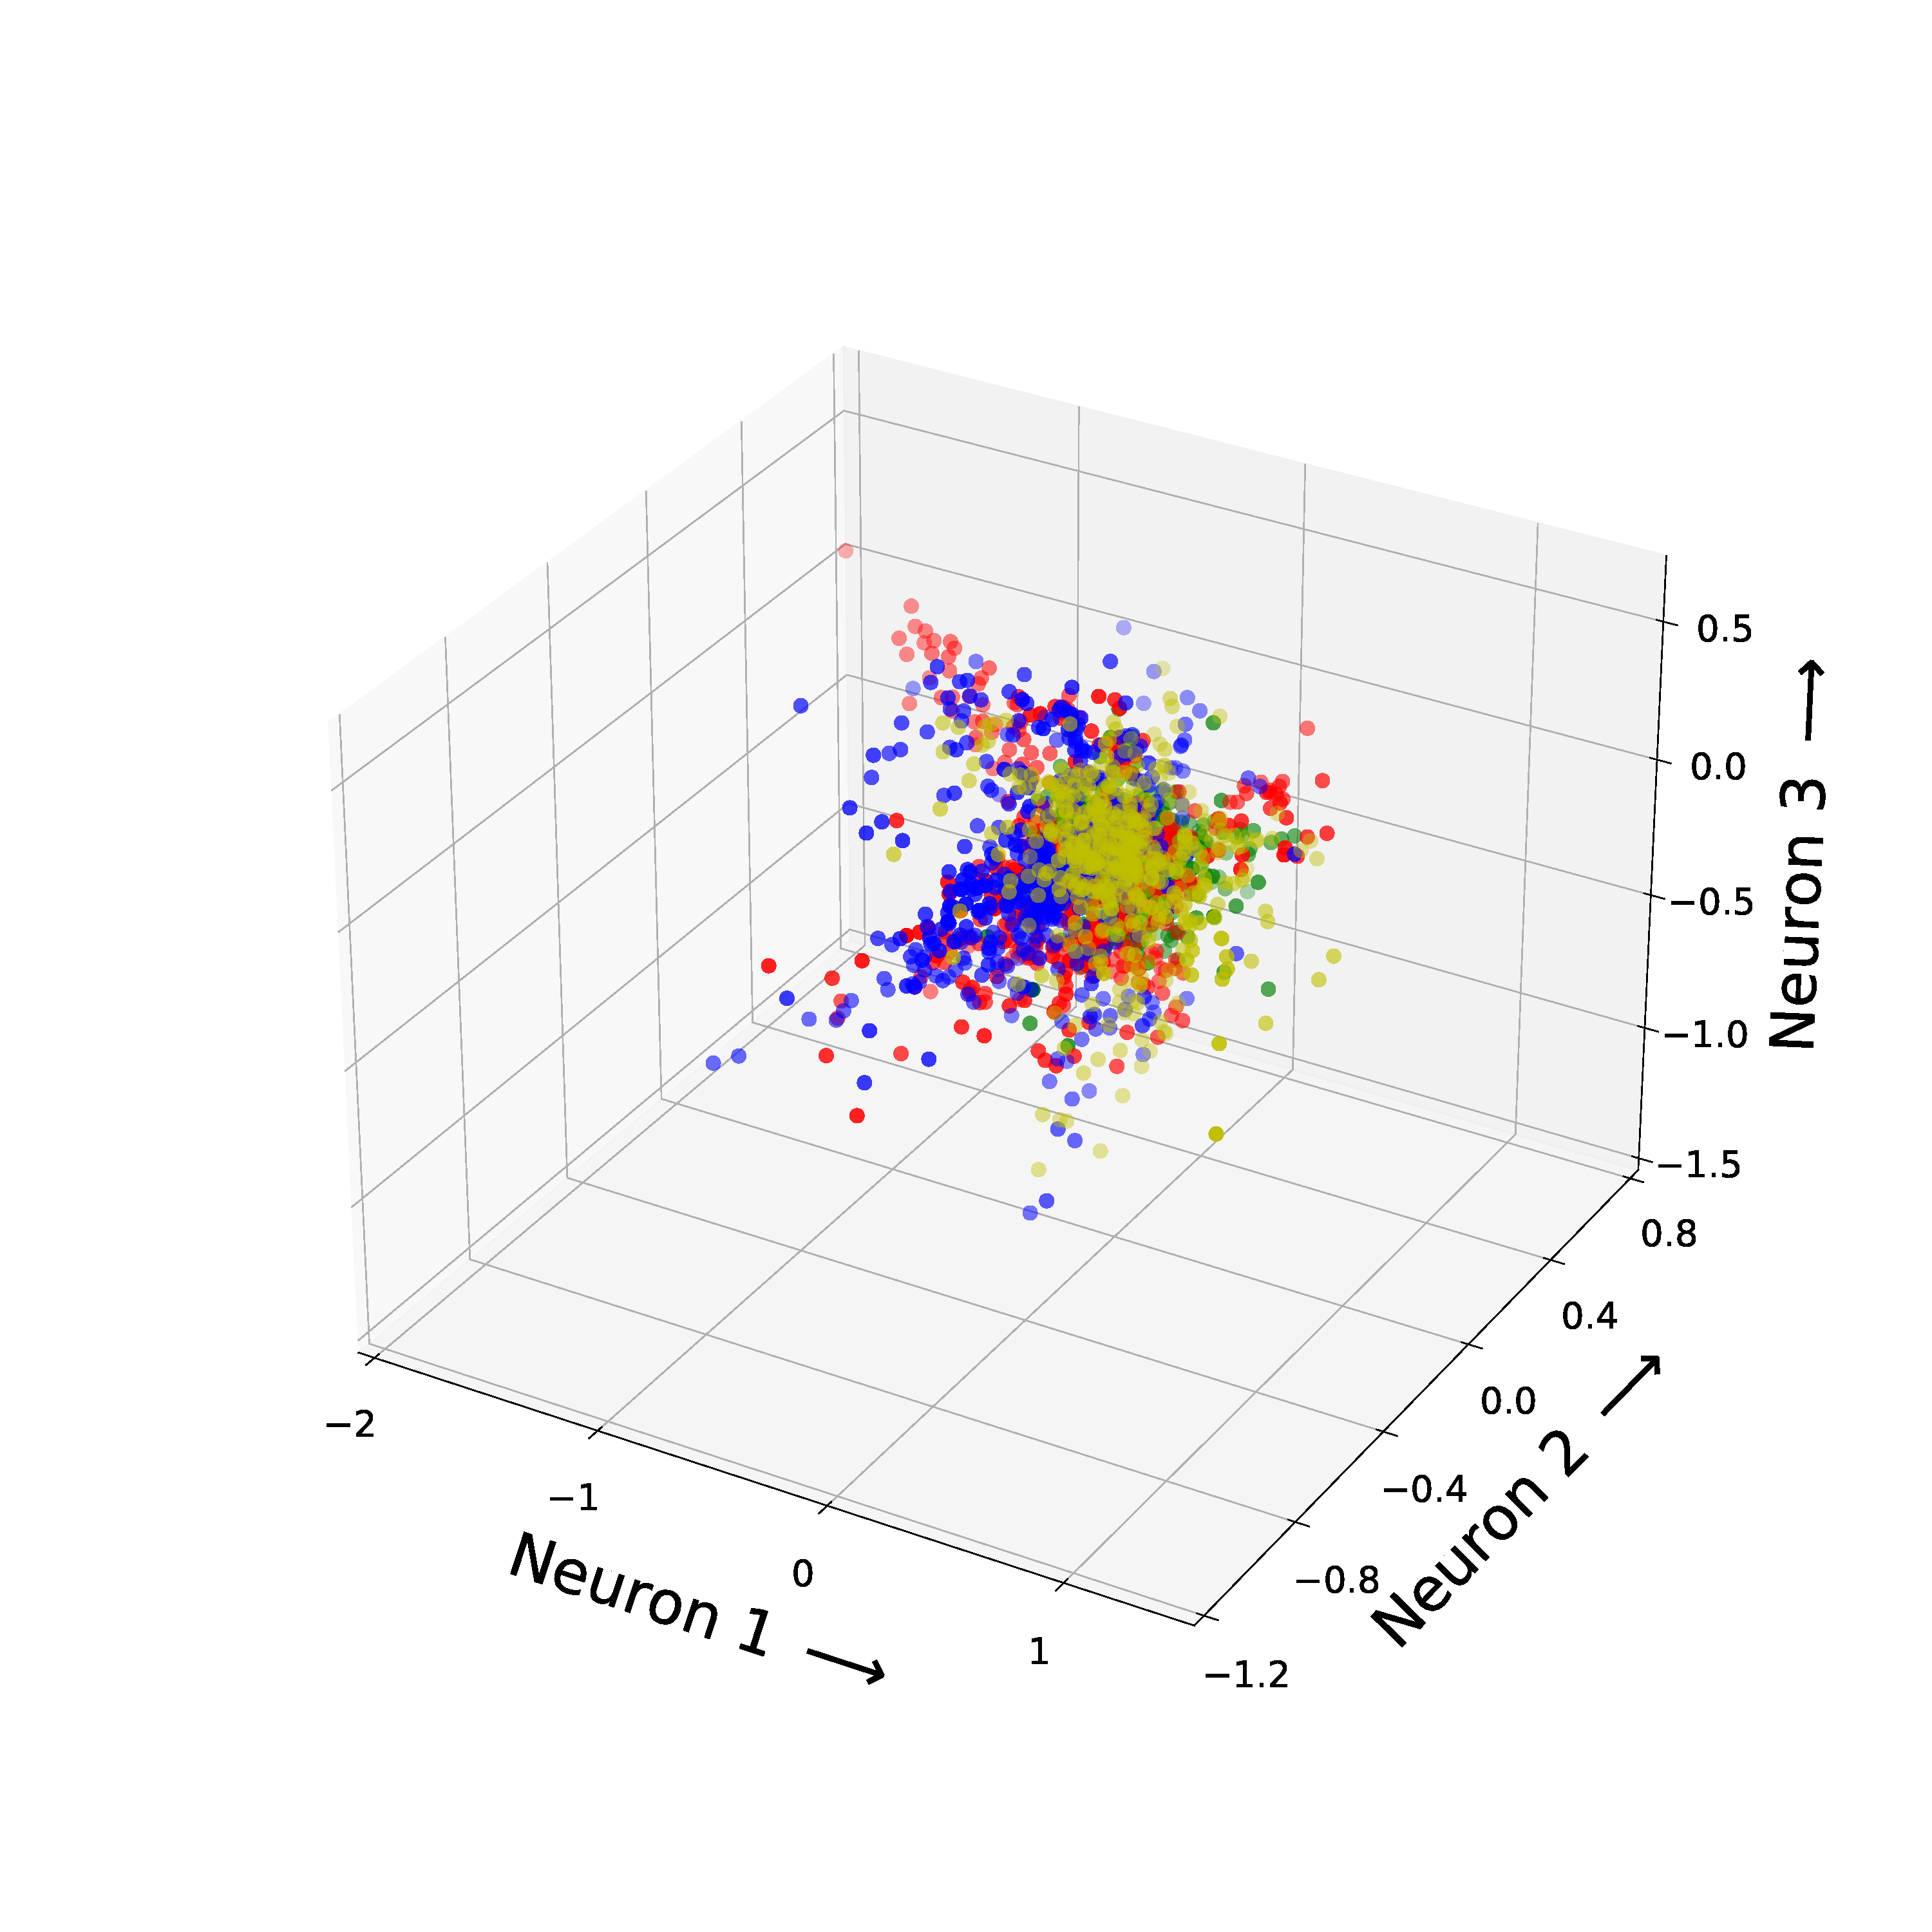
\includegraphics[width=.48\textwidth]{GAMMA_Influence_dummy_distribution/Dummy_distribution_0_GAMMA_0_001.pdf}
  \hspace{.4cm}
  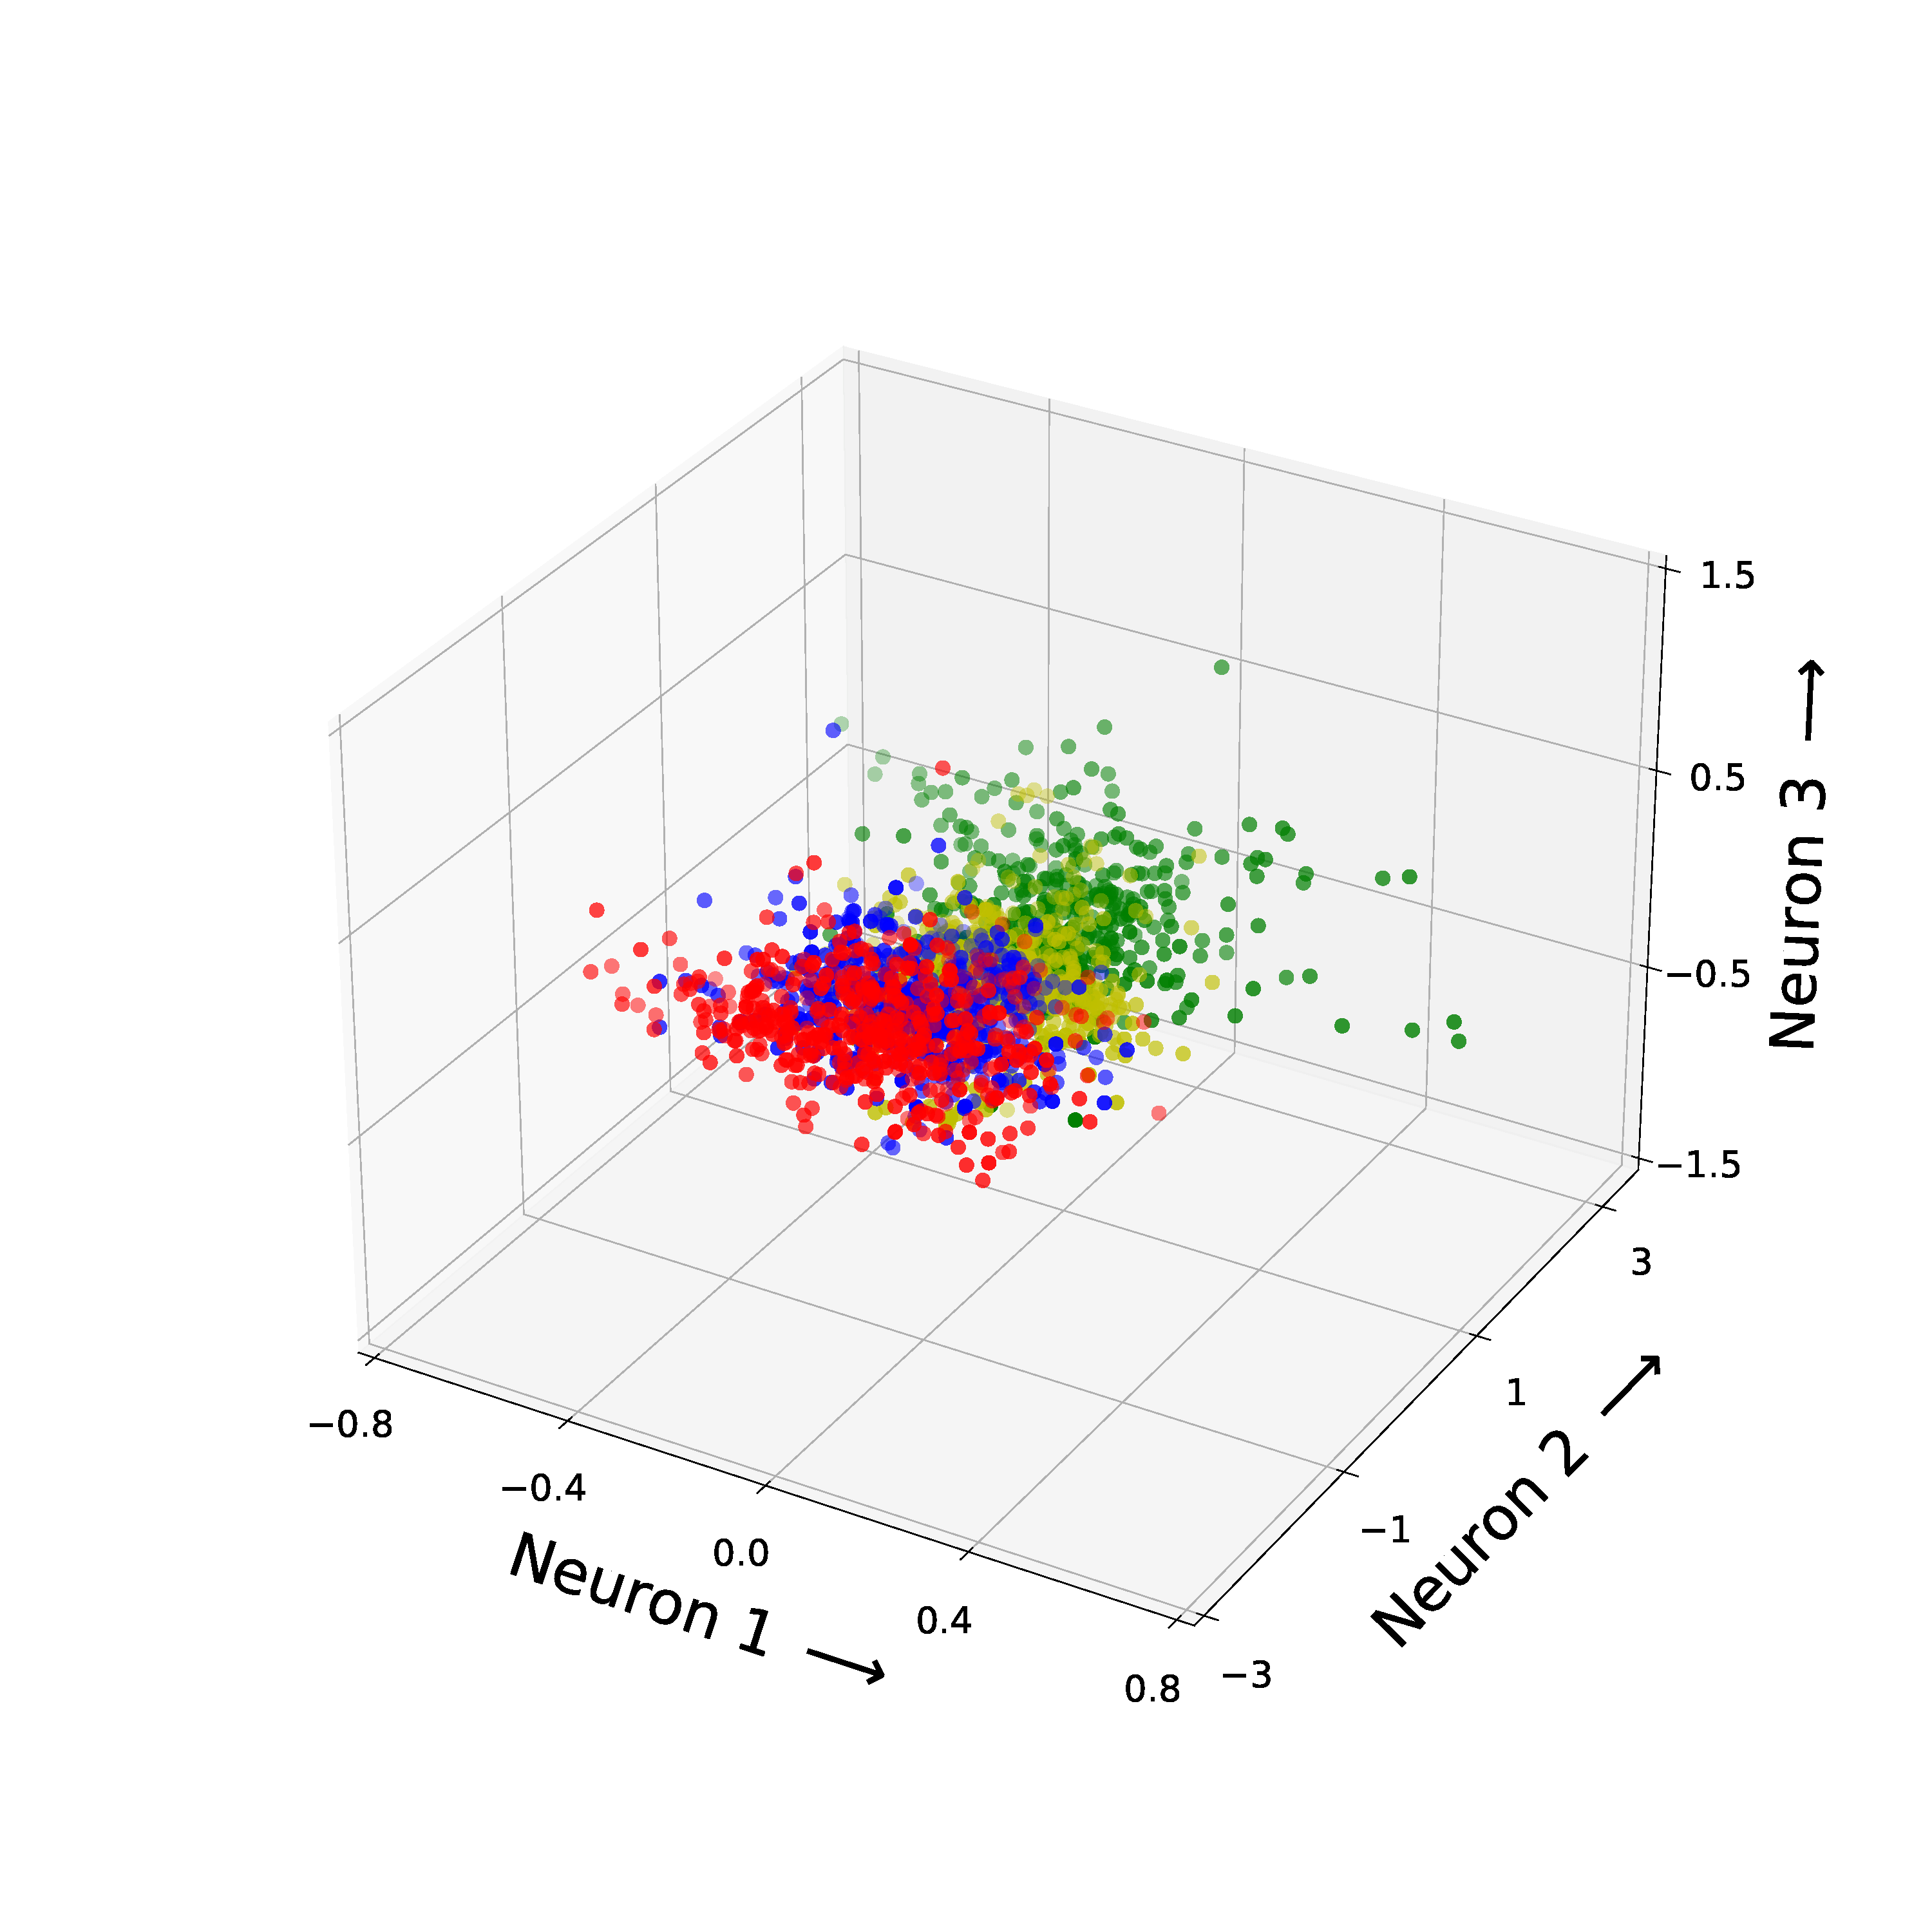
\includegraphics[width=.48\textwidth]{GAMMA_Influence_dummy_distribution/Dummy_distribution_8_GAMMA_0_001.pdf}

  \vspace{.1cm}

  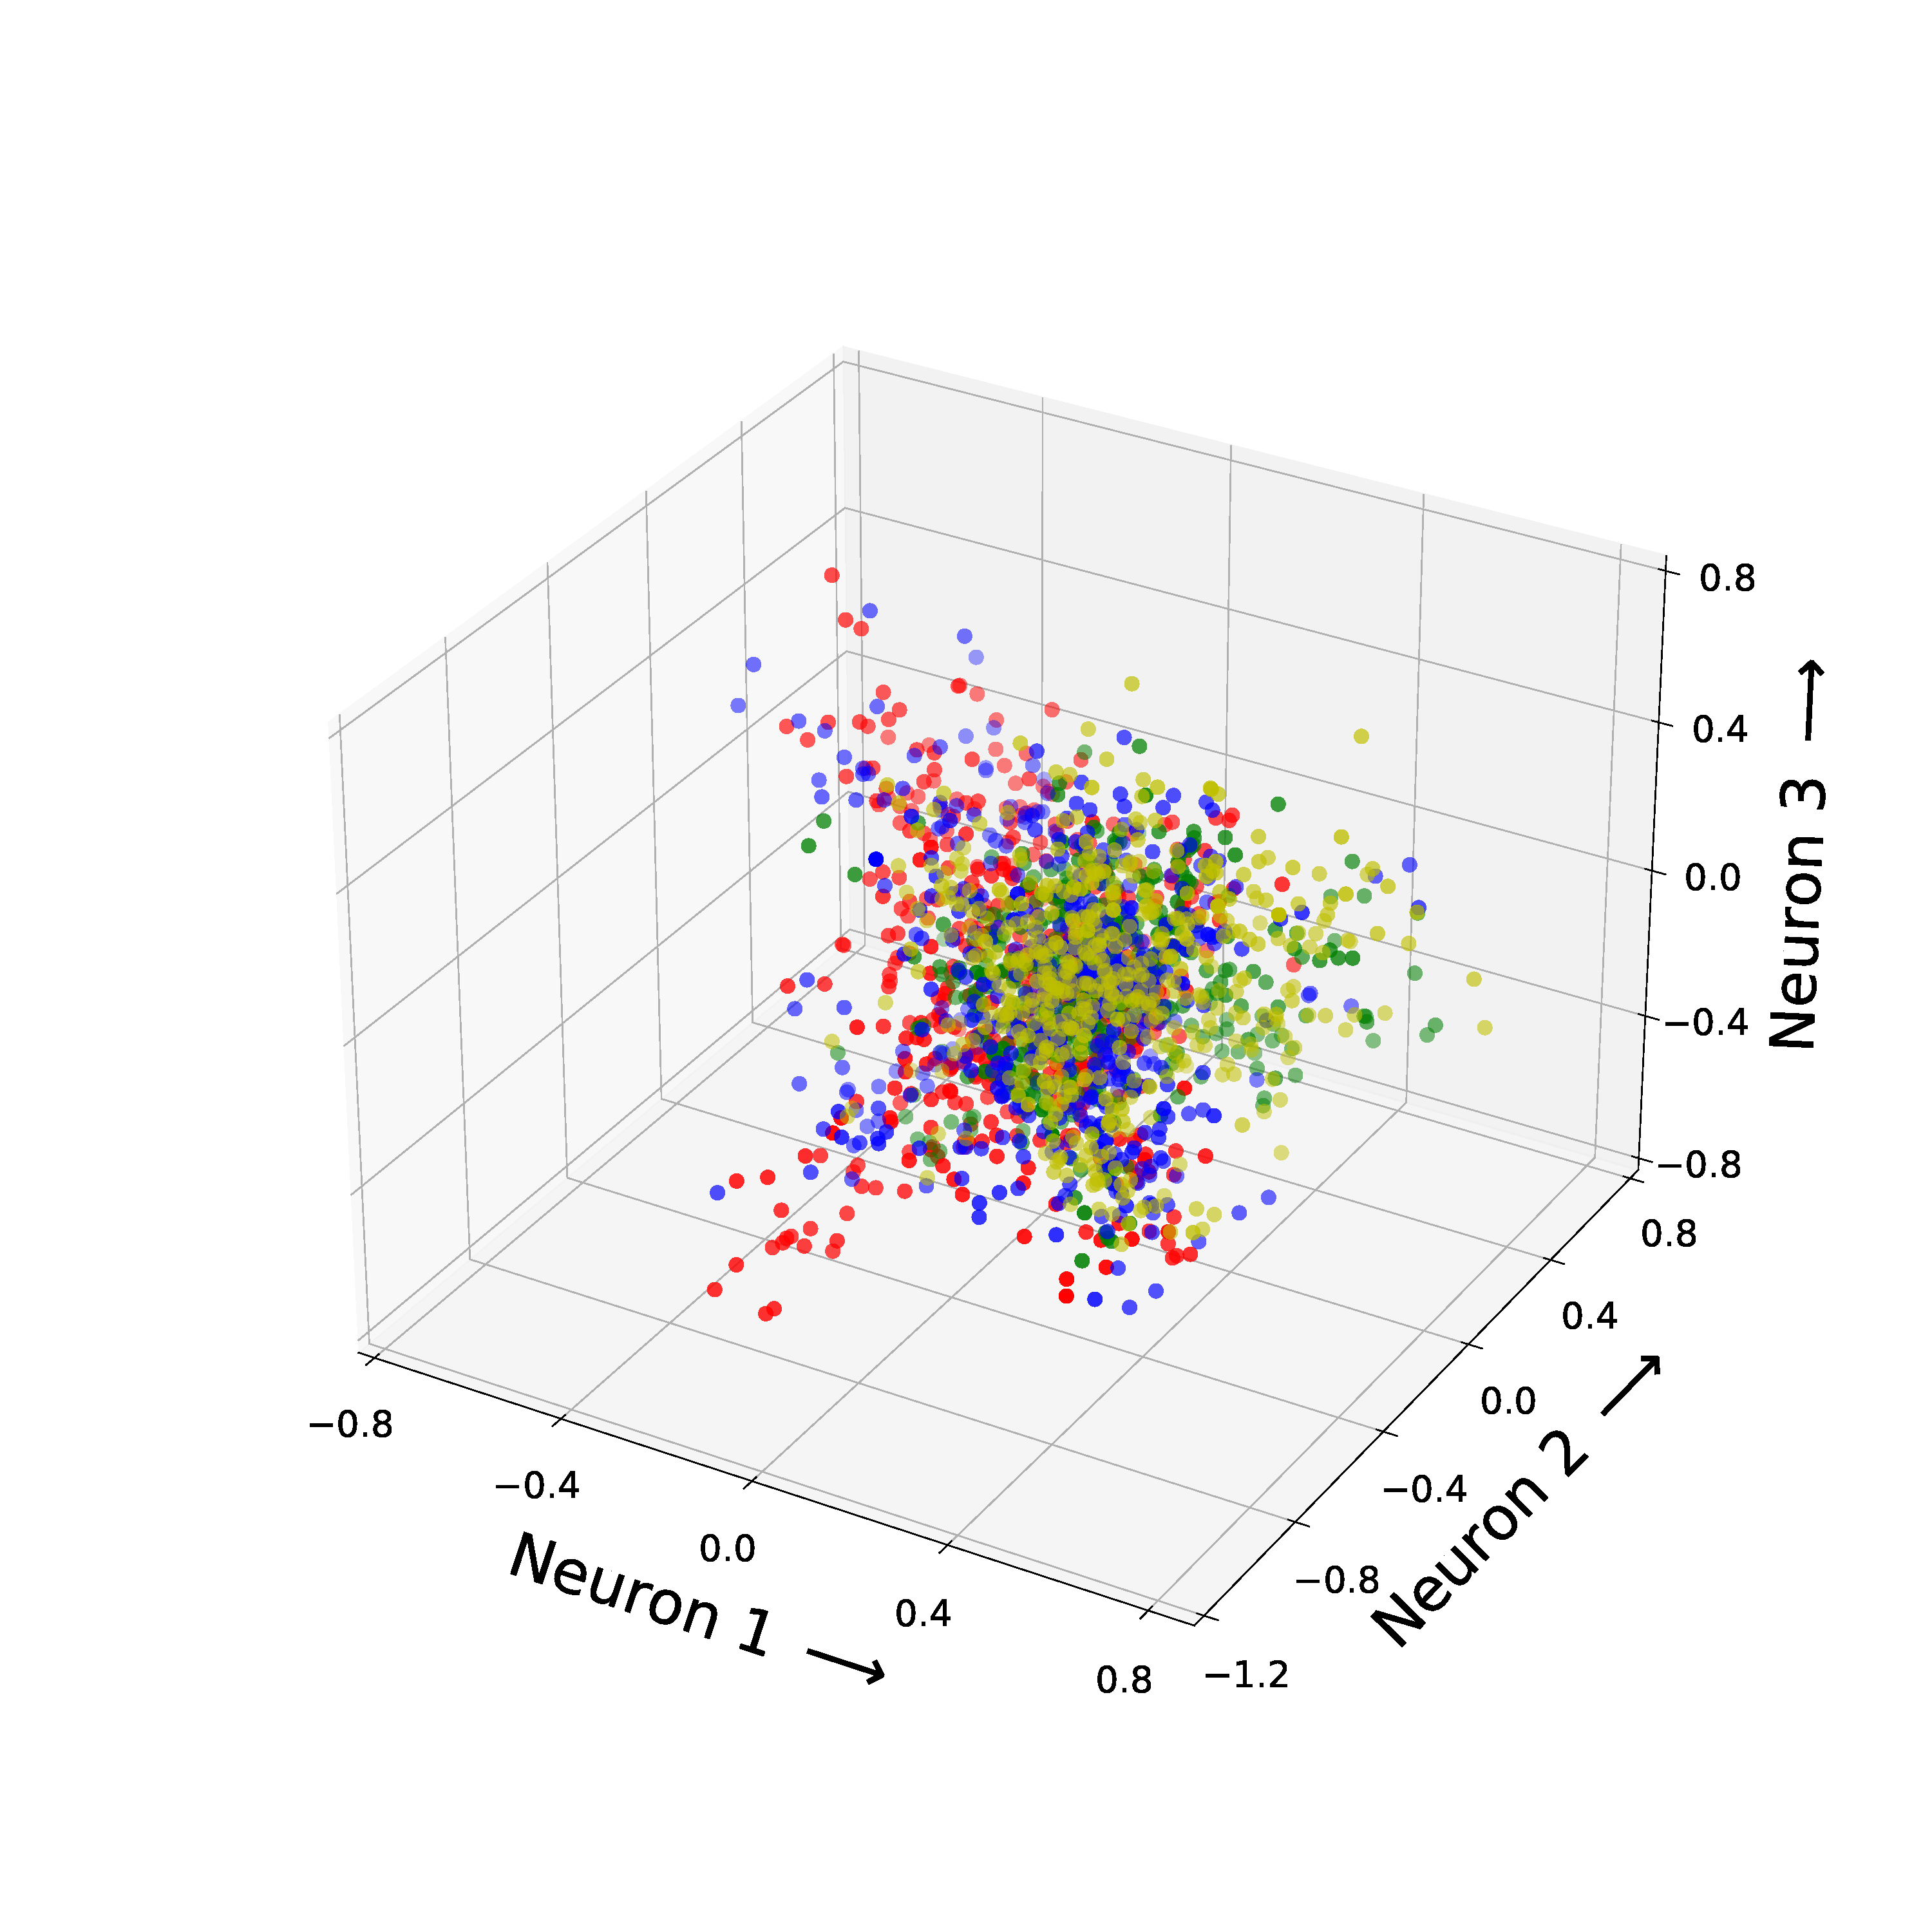
\includegraphics[width=.48\textwidth]{GAMMA_Influence_dummy_distribution/Dummy_distribution_0_GAMMA_0_1.pdf}
  \hspace{.4cm}
  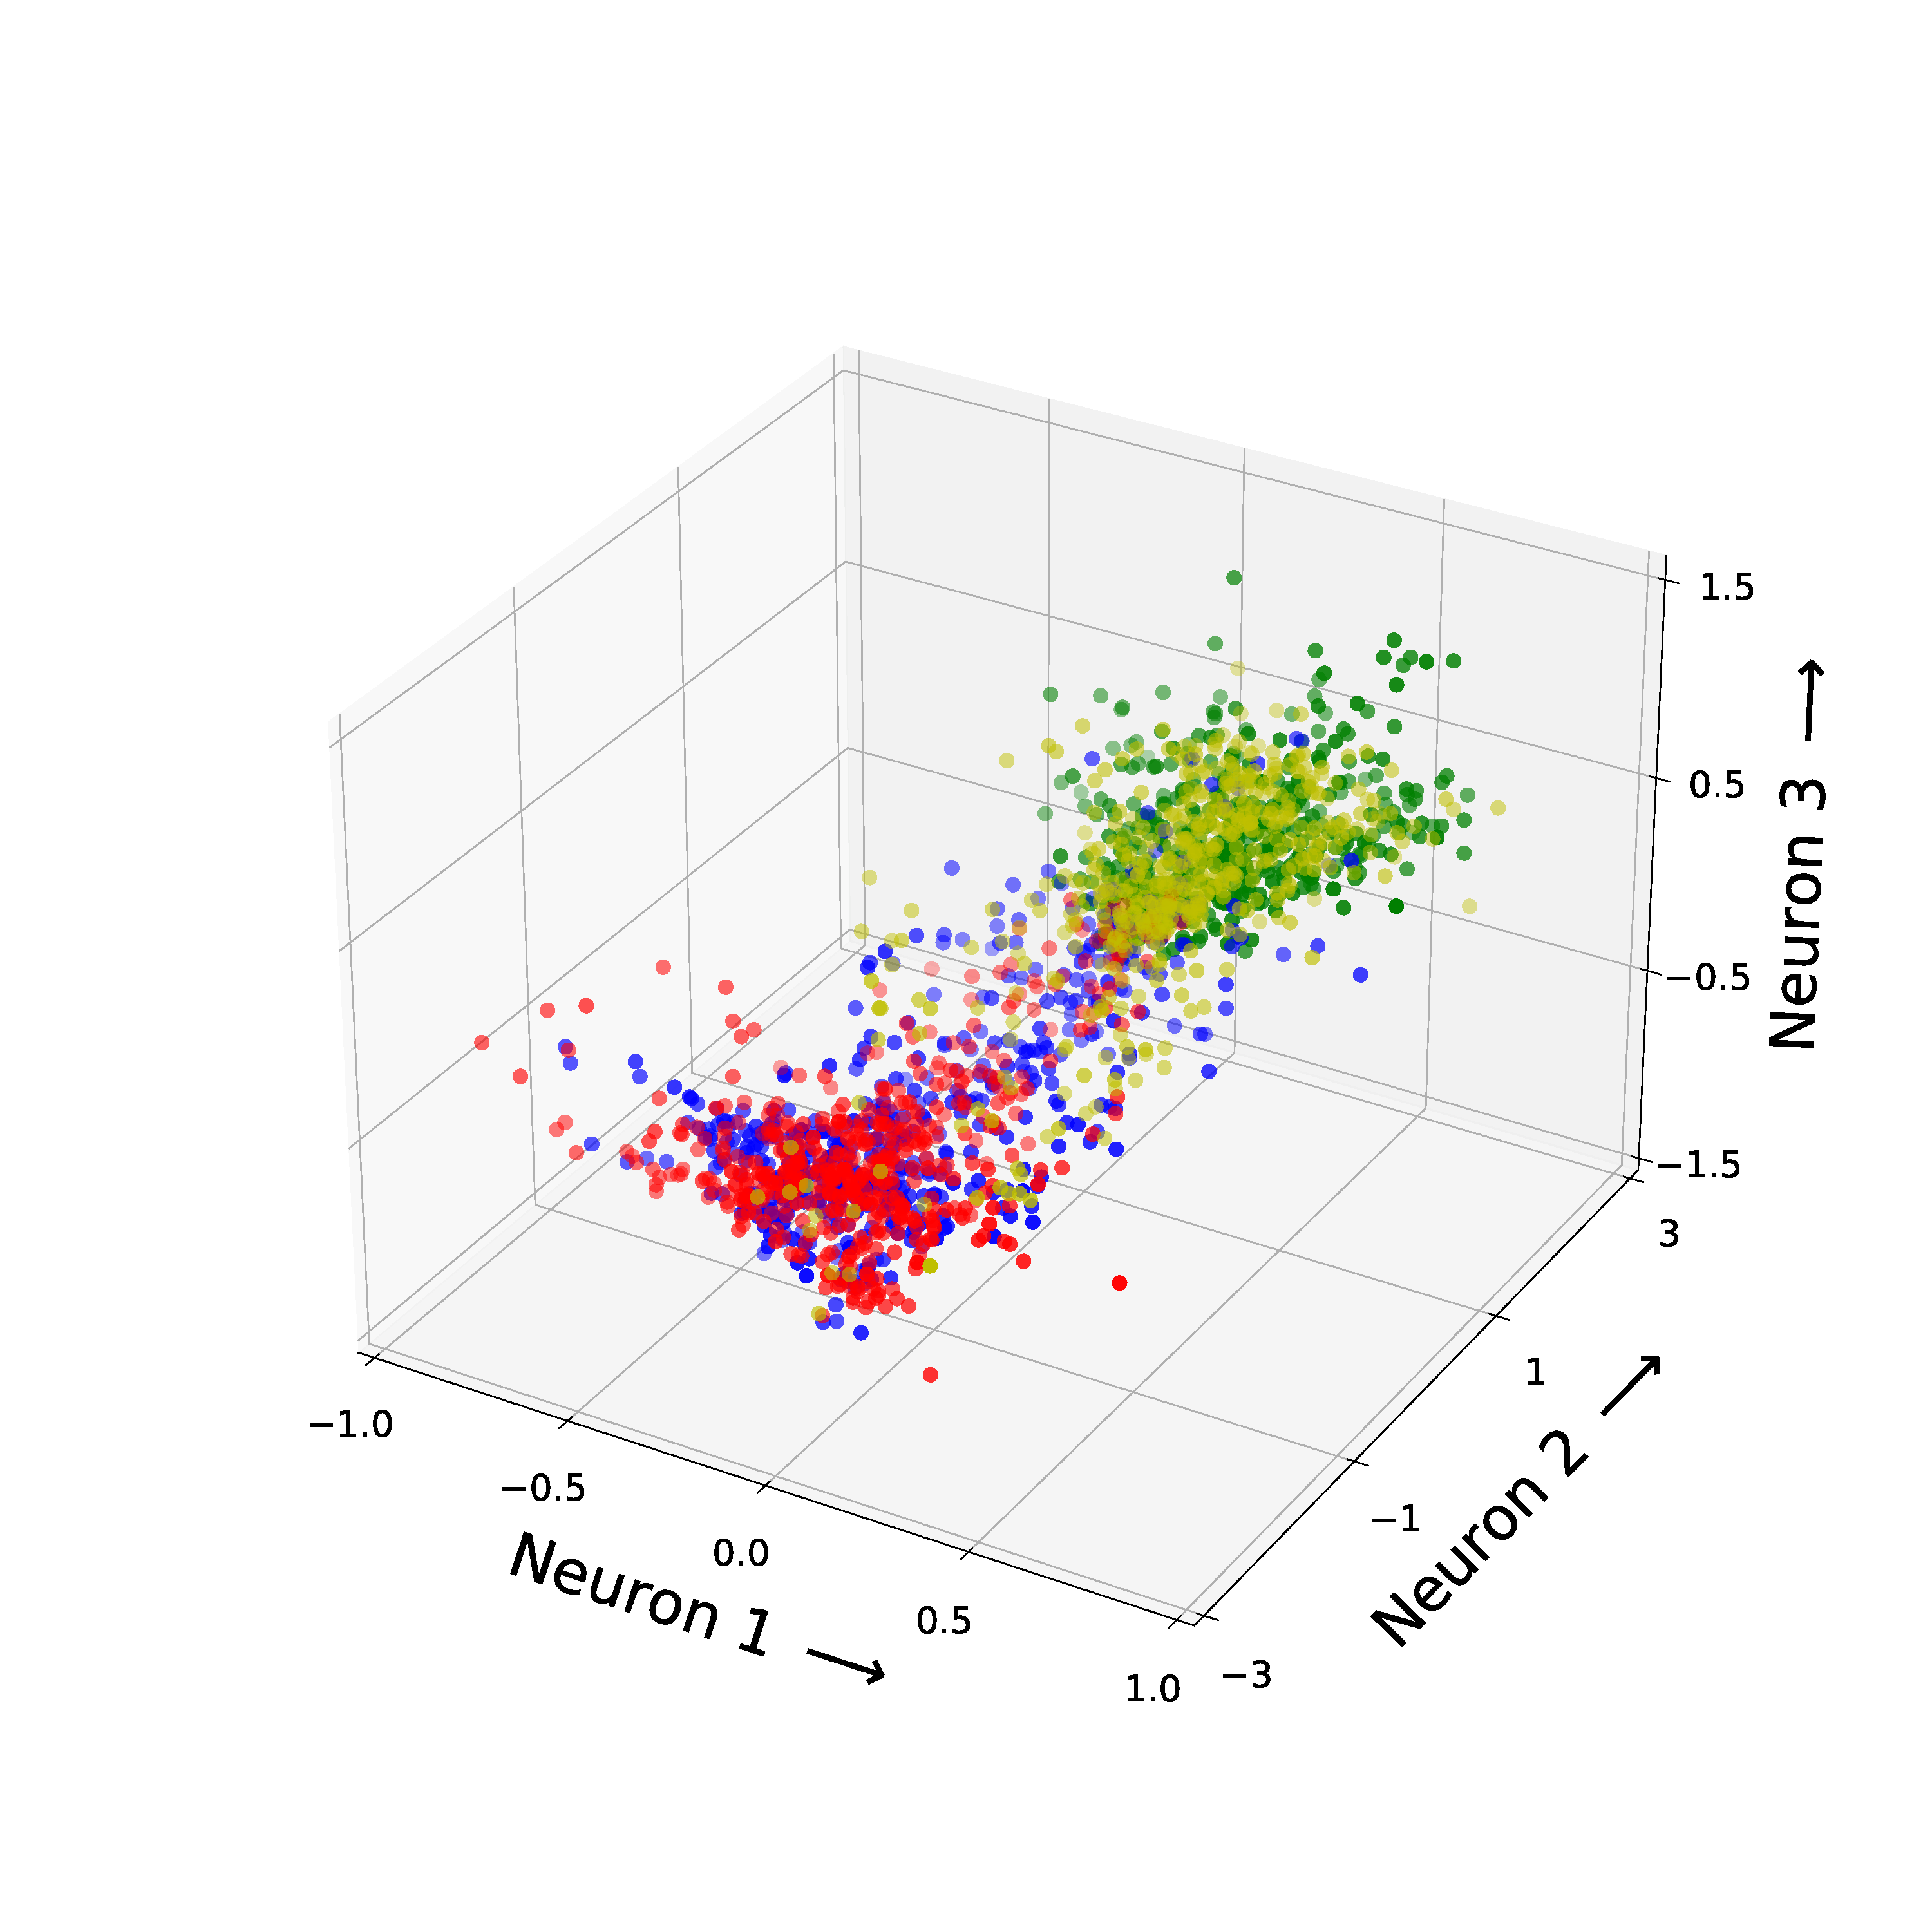
\includegraphics[width=.48\textwidth]{GAMMA_Influence_dummy_distribution/Dummy_distribution_8_GAMMA_0_1.pdf}

  \vspace{.1cm}

  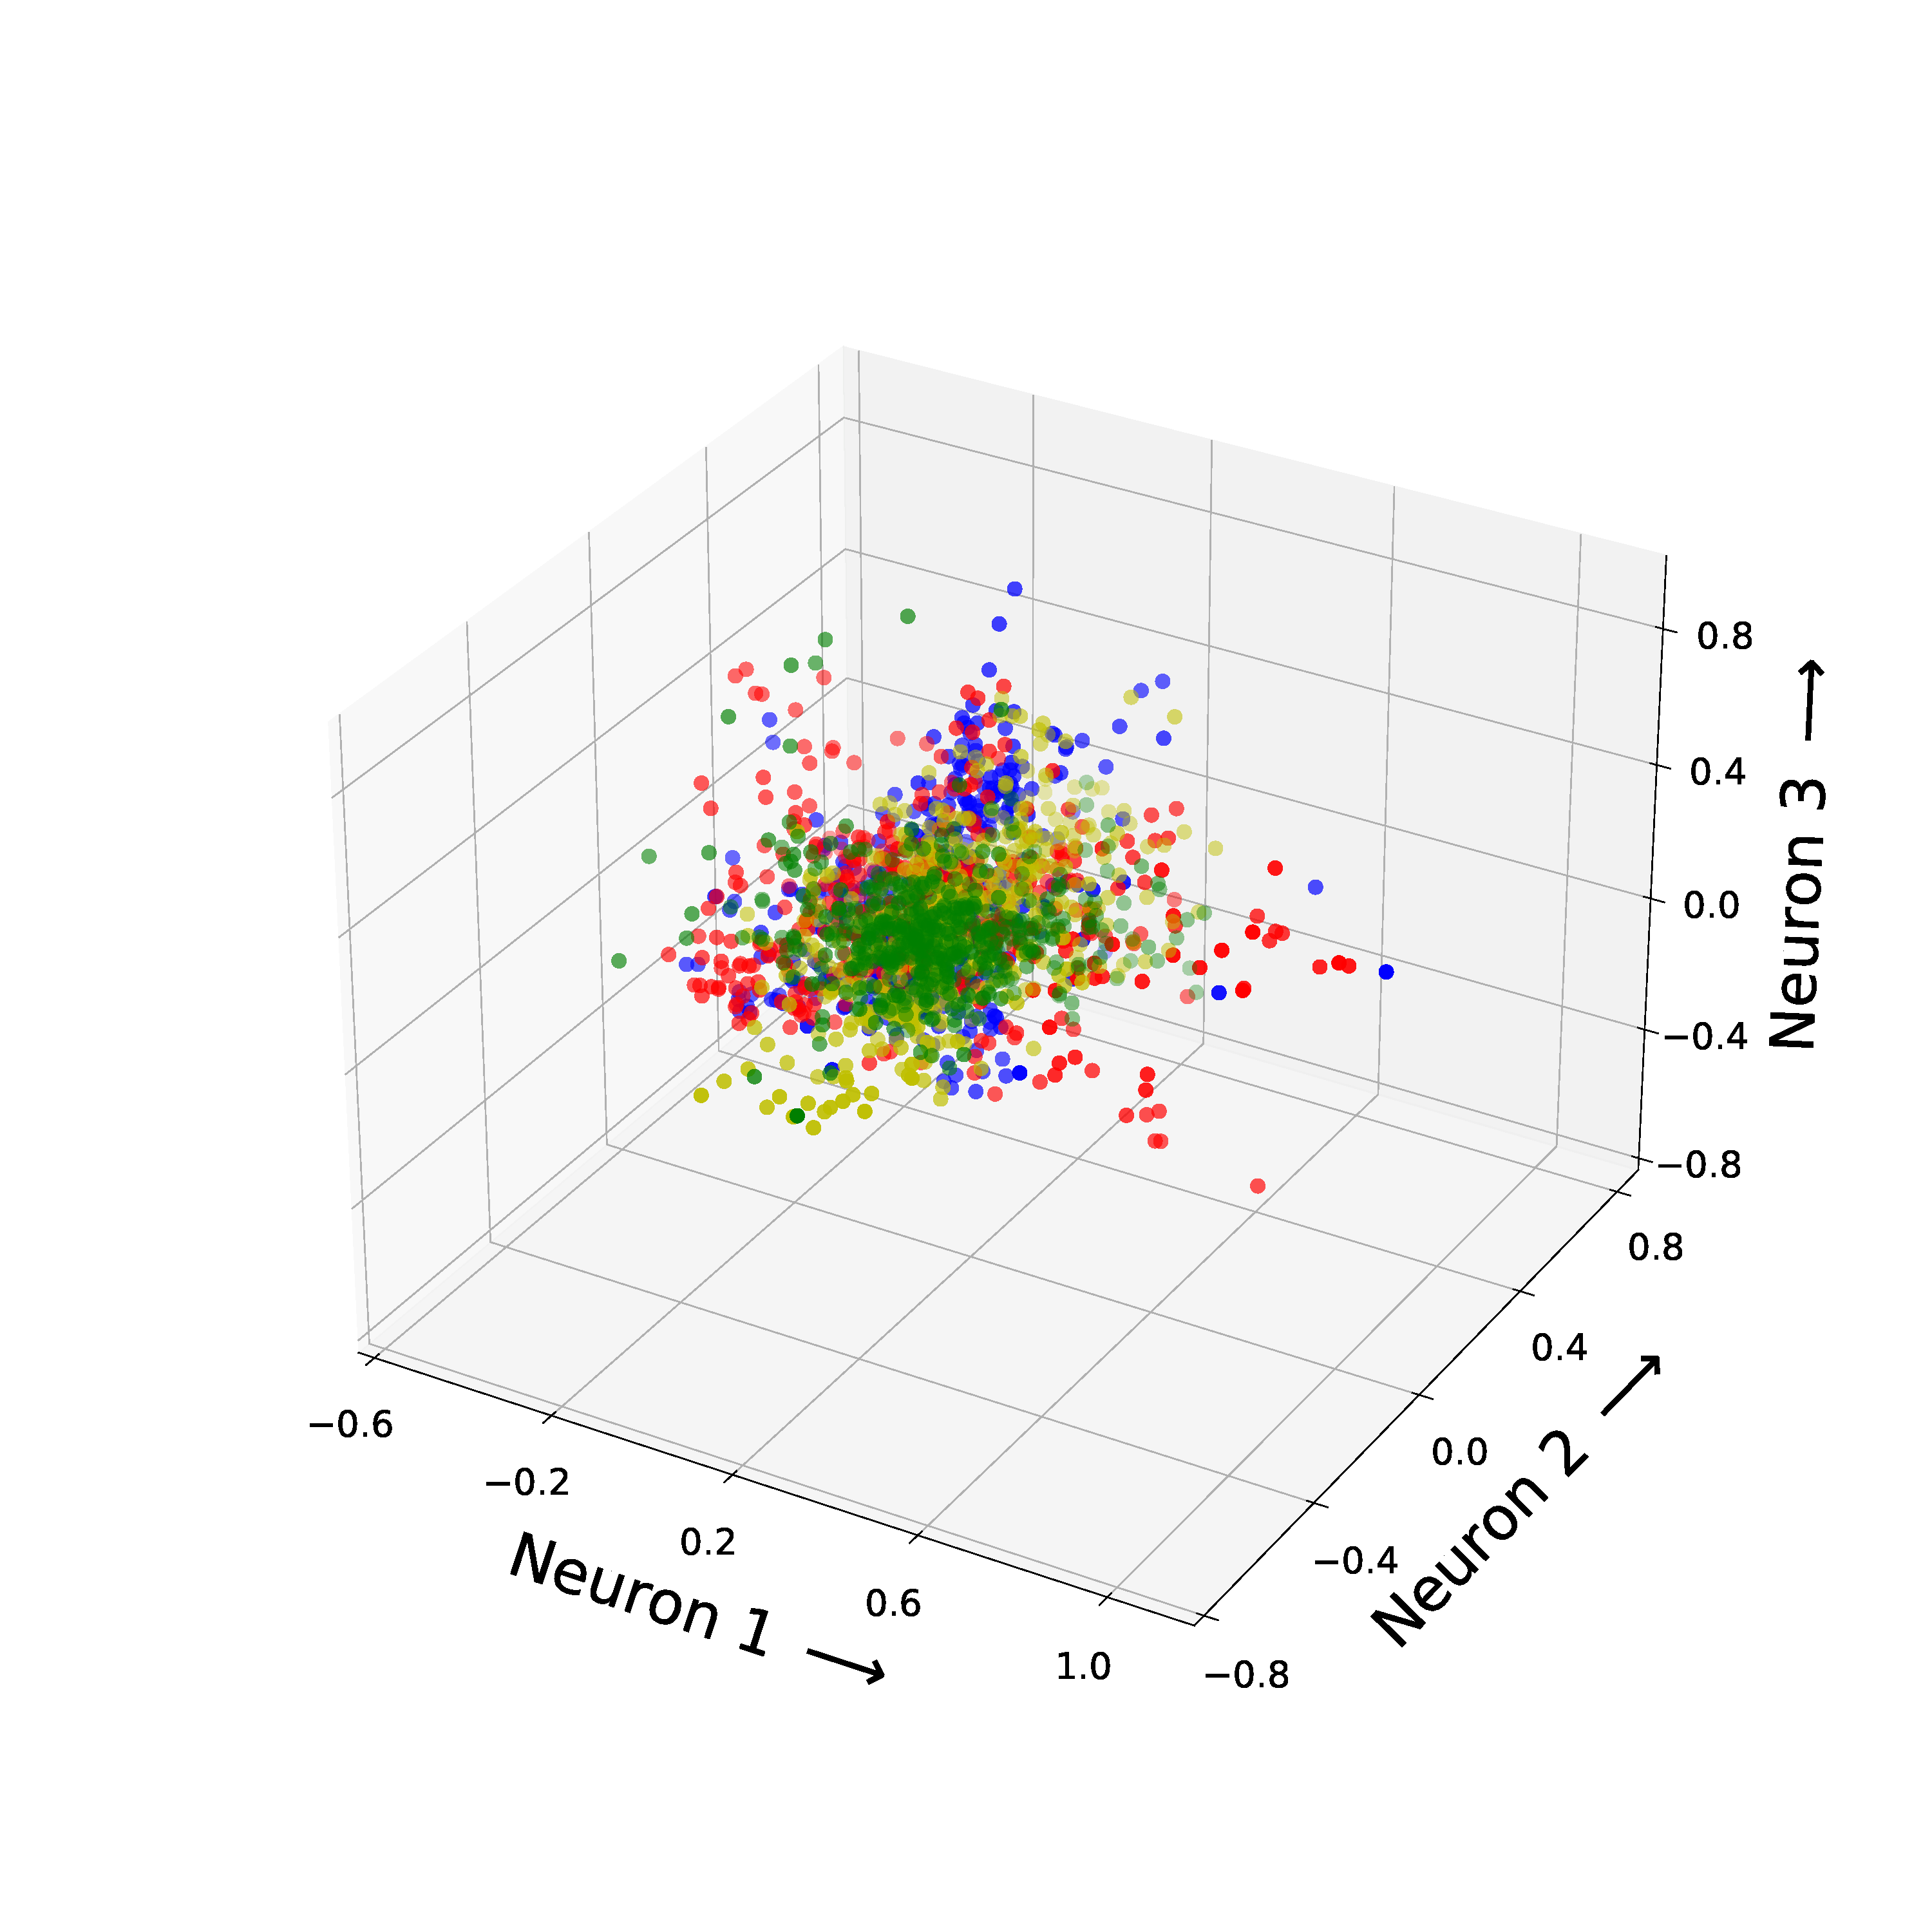
\includegraphics[width=.48\textwidth]{GAMMA_Influence_dummy_distribution/Dummy_distribution_0_GAMMA_20.pdf}
  \hspace{.4cm}
  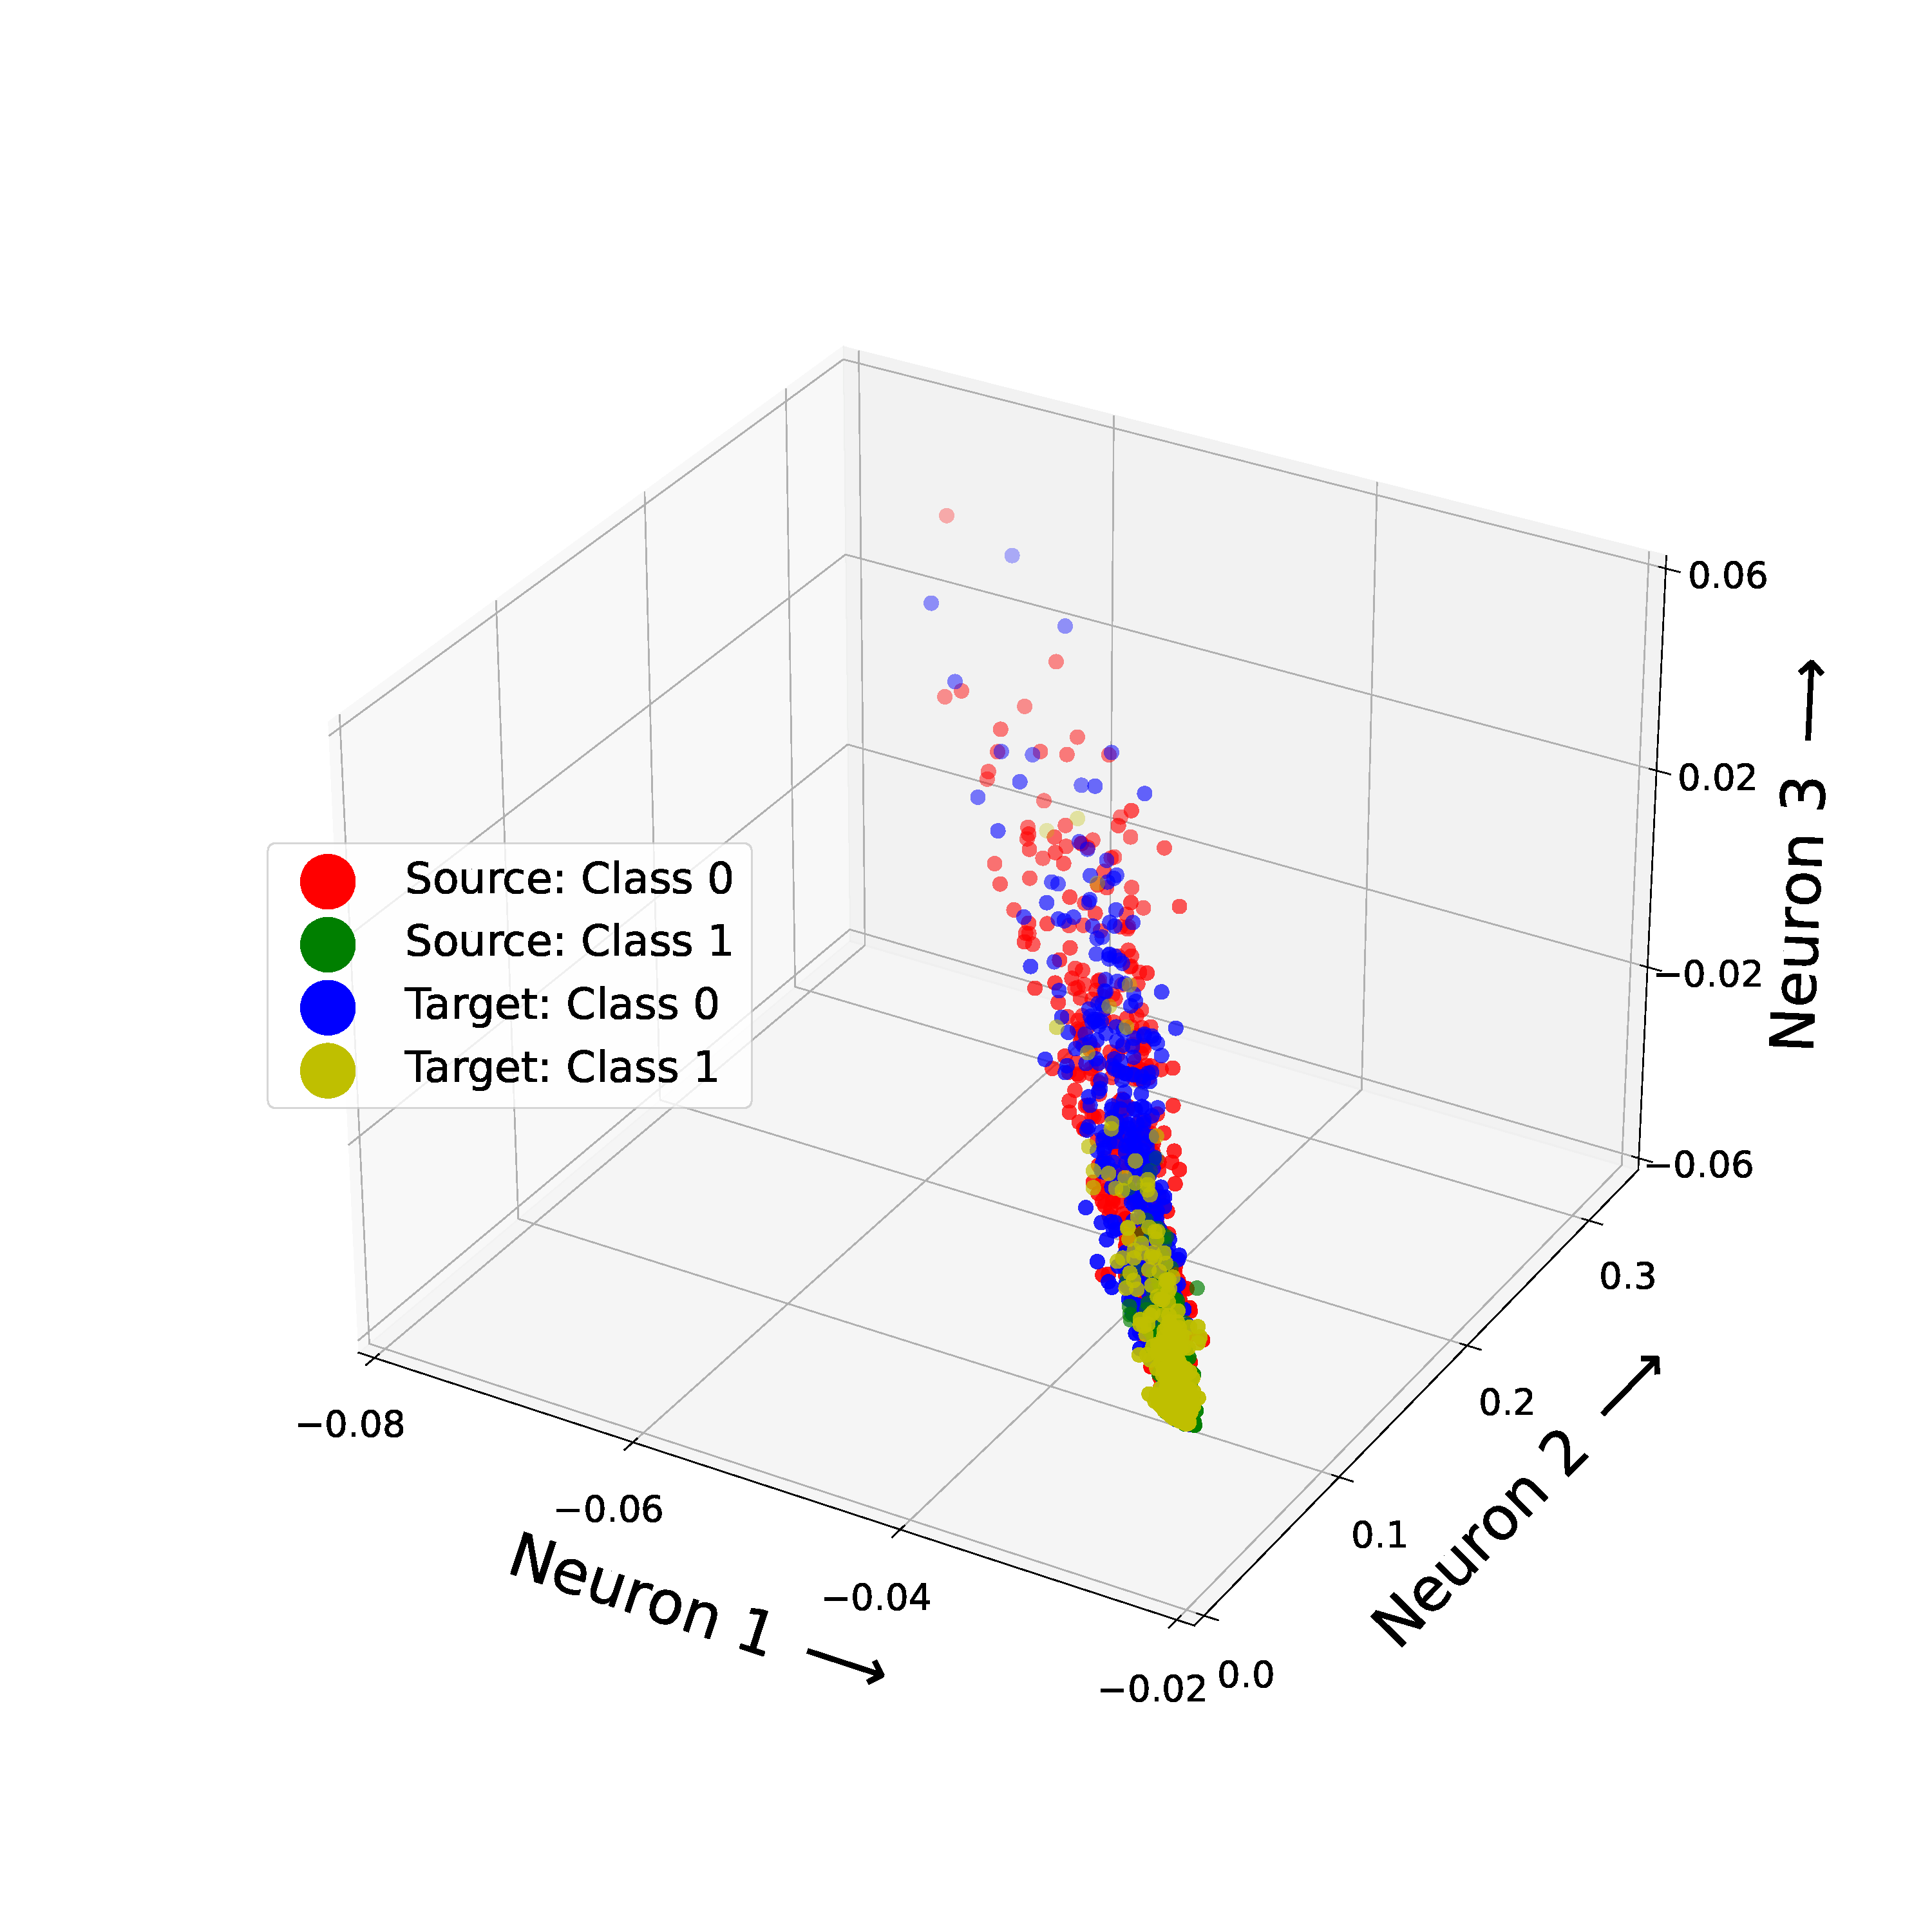
\includegraphics[width=.48\textwidth]{GAMMA_Influence_dummy_distribution/Dummy_distribution_8_GAMMA_20.pdf}
 

  \caption{Data distribution: Influence of GAMMA on Training, GAMMA = 0.05 (top), GAMMA = 0,4 (middle), GAMMA = 20 (bottom), Epoch = 0 (left) , Epoch = 8 (right)}
  \label{fig:point_cloud_mmd}
\end{figure}


\begin{figure}[htp]
  \centering
  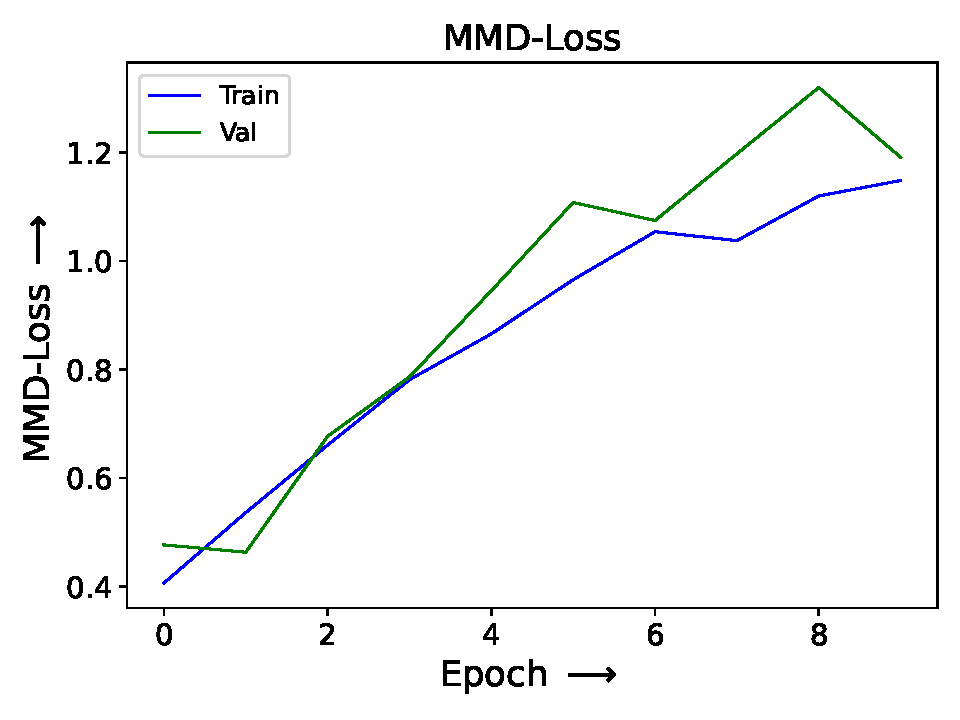
\includegraphics[width=.47\textwidth]{GAMMA_Influence_dummy_curve/MMD_Loss_GAMMA_0_001.pdf}
  \hspace{.3cm}
  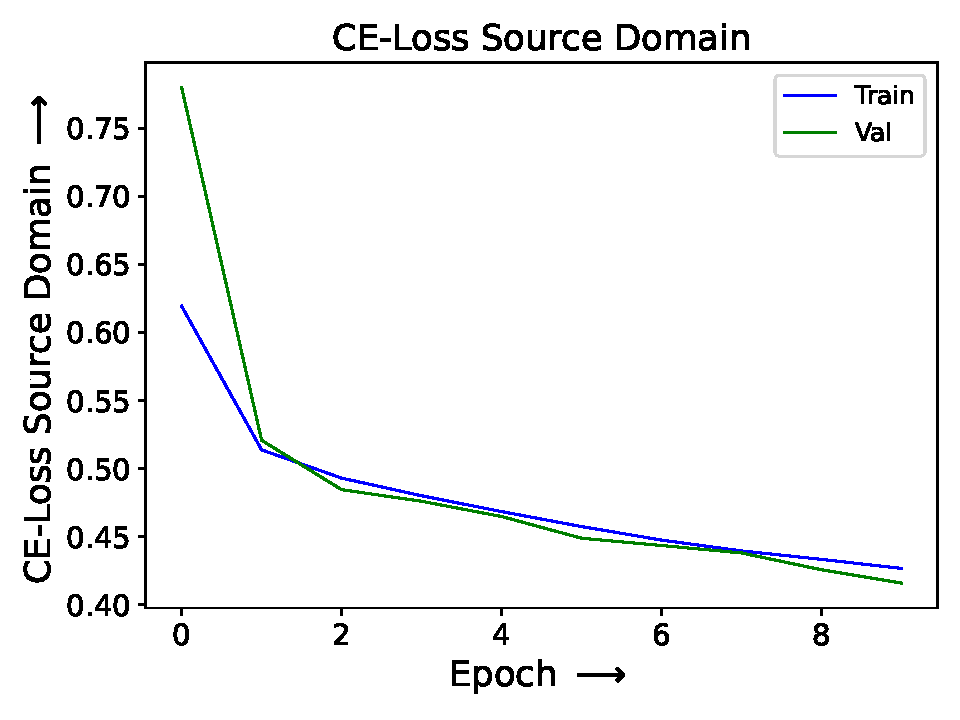
\includegraphics[width=.47\textwidth]{GAMMA_Influence_dummy_curve/CE_Loss_Source_Domain_GAMMA_0_001.pdf}

  \vspace{.1cm}

  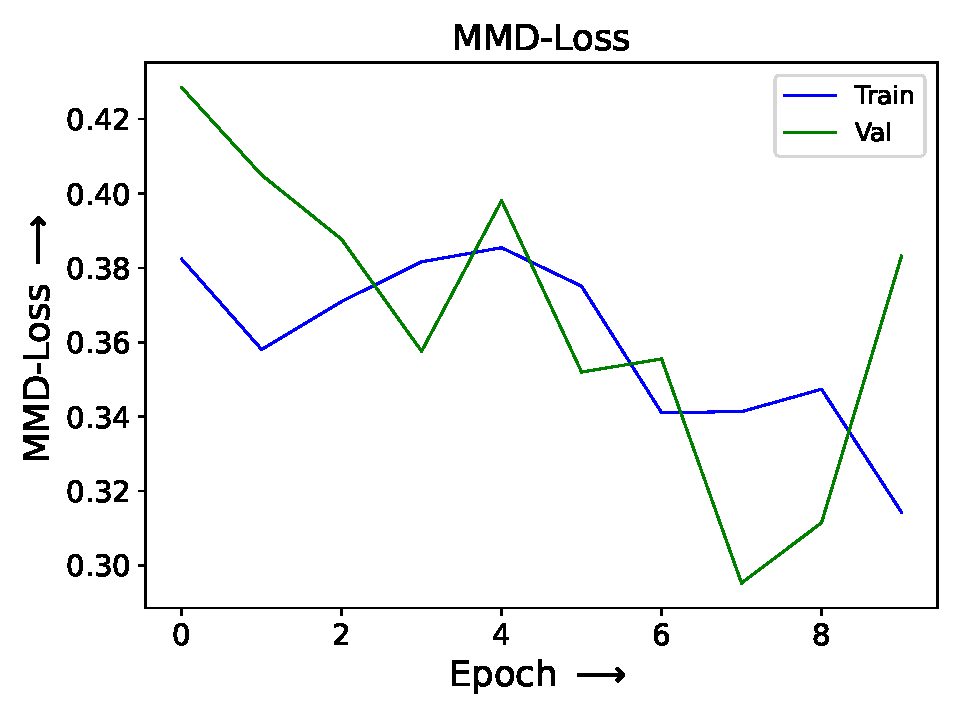
\includegraphics[width=.47\textwidth]{GAMMA_Influence_dummy_curve/MMD_Loss_GAMMA_0_1.pdf}
  \hspace{.3cm}
  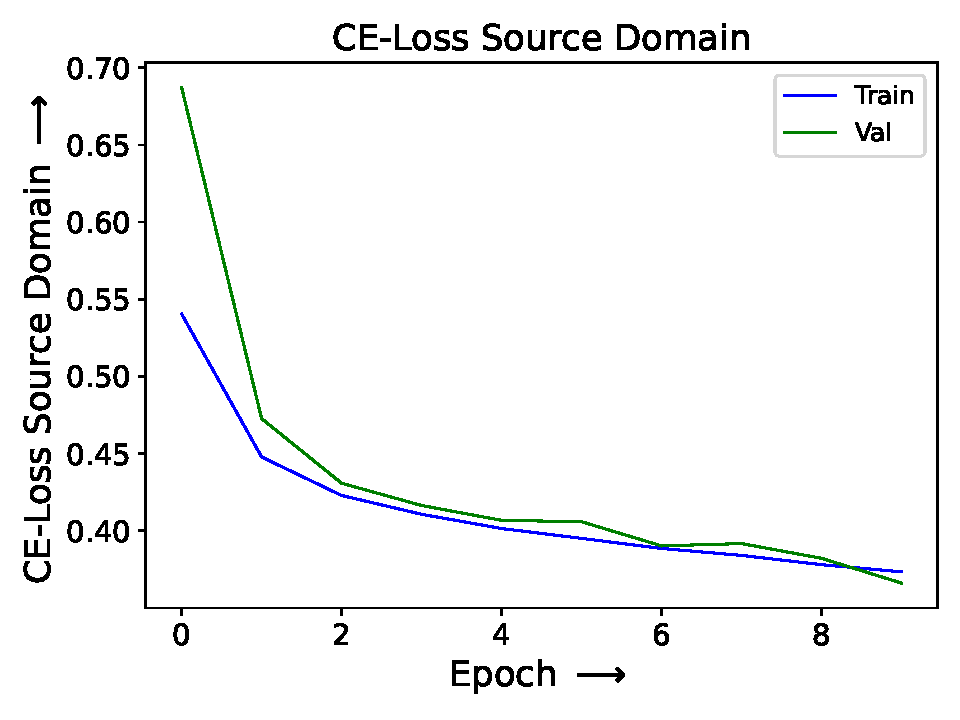
\includegraphics[width=.47\textwidth]{GAMMA_Influence_dummy_curve/CE_Loss_Source_Domain_GAMMA_0_1.pdf}

  \vspace{.1cm}

  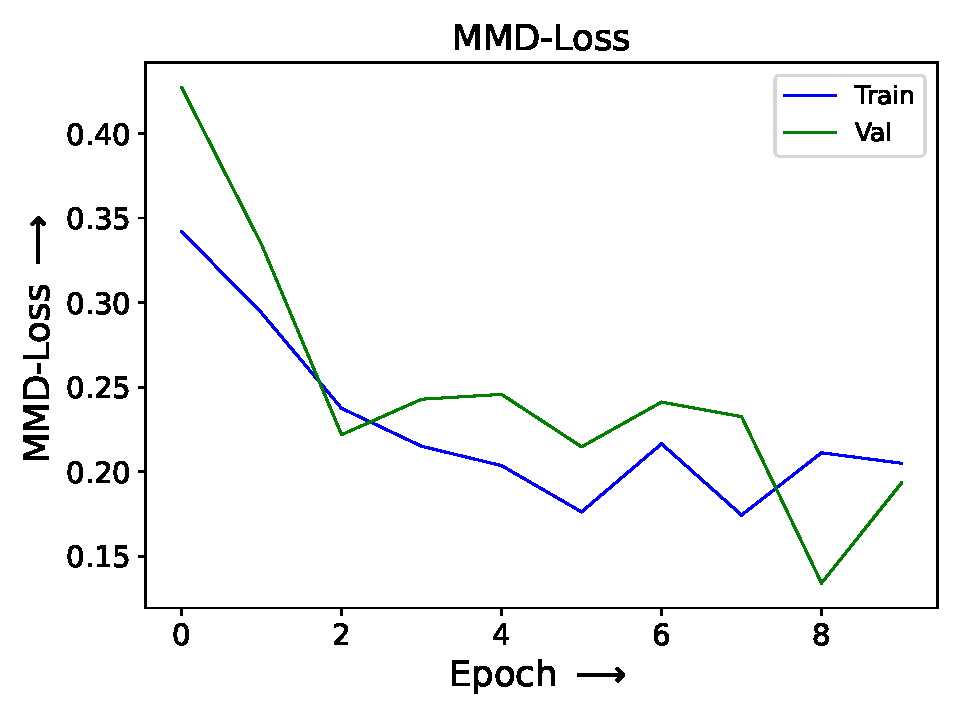
\includegraphics[width=.47\textwidth]{GAMMA_Influence_dummy_curve/MMD_Loss_GAMMA_20.pdf}
  \hspace{.1cm}
  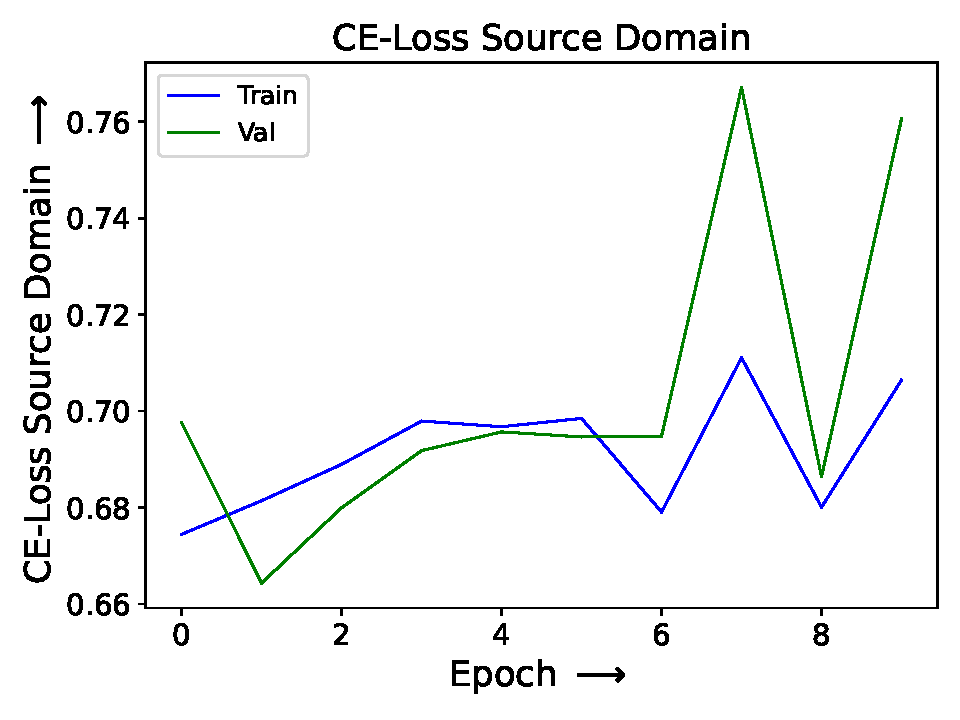
\includegraphics[width=.47\textwidth]{GAMMA_Influence_dummy_curve/CE_Loss_Source_Domain_GAMMA_20.pdf}

  \caption{MMD- and source CE-loss: Influence of GAMMA on Training: GAMMA = 0.001 (top), GAMMA = 0.1 (middle), GAMMA = 20 (bottom), Epoch 0 (left), Epoch 8 (right)}
  \label{fig:learning_curves_influence_mmd_feature_extractor}
\end{figure}

\subsection{Domain Adaption Performance of a Labeled MMD-loss} \label{sec:Differences of labeled and unlabeled MMD loss}

In the unlabeled MMD-loss, the target labels are unknown. Therefore, the intra- and inter-class distance between source and target samples are minimized equally. Obviously, this increases the compactness but reduces the class separability in both domains. In the literature some approaches extend the unlabeled MMD-based model training with a distance-based optimization, which includes target labels \cite{Pandhare2021}. Usually those approaches restrict the supervised training to the source domain. In this section a novel labeled MMD-loss is presented which includes target labels but restricts the supervised training to the source domain. The domain discrepancy between source and target samples of similar and different classes is optimized separately. The labeled MMD-loss minimizes the intra-class discrepancy and maximizes the inter-class discrepancy between the domains. This separate consideration of class distances allows a simultaneous improvement of class separability and compactness. A weighted loss is applied which combines the source CE-loss, the intra-class and the inter-class MMD-loss. This approach expects additional hyperparameter, which need to be defined beforehand. The hyperparameters GAMMA\_Intra\_Class and GAMMA\_Inter\_Class are used to balance the training scope of maximizing the intra-class distance and minimizing the inter-class distance and source CE-loss:

\begin{equation}
\begin{split}
    \mbox{Total Loss} = & \mbox{GAMMA\_Intra\_Class}  \cdot \mbox{MMD\_Loss\_Intra\_Class} + \\
                              &\mbox{GAMMA\_Inter\_Class} \cdot \mbox{MMD\_Loss\_Inter\_Class} + \mbox{CE\_Loss}.
\end{split}
\end{equation}

 The MMD-loss which includes the target labels is named "labeled MMD-loss" and otherwise "unlabeled MMD-loss". Again, fig. \ref{fig:point_cloud_labeled_unlabeled_mmd} visualizes the latent feature representation in FC2. Throughout the training, the labeled MMD-loss is able to reduce the domain discrepancy while increasing the separability and compactness of the classes in both domains. This simplifies the classification problem and makes the model optimization less prone to find a trivial solution, in which the latent feature representation of all samples collapse at one point or a needle-like subspace. In this experiment, 20\% of target labels were used in labeled MMD-loss.
\begin{figure}[htp]
  \centering
  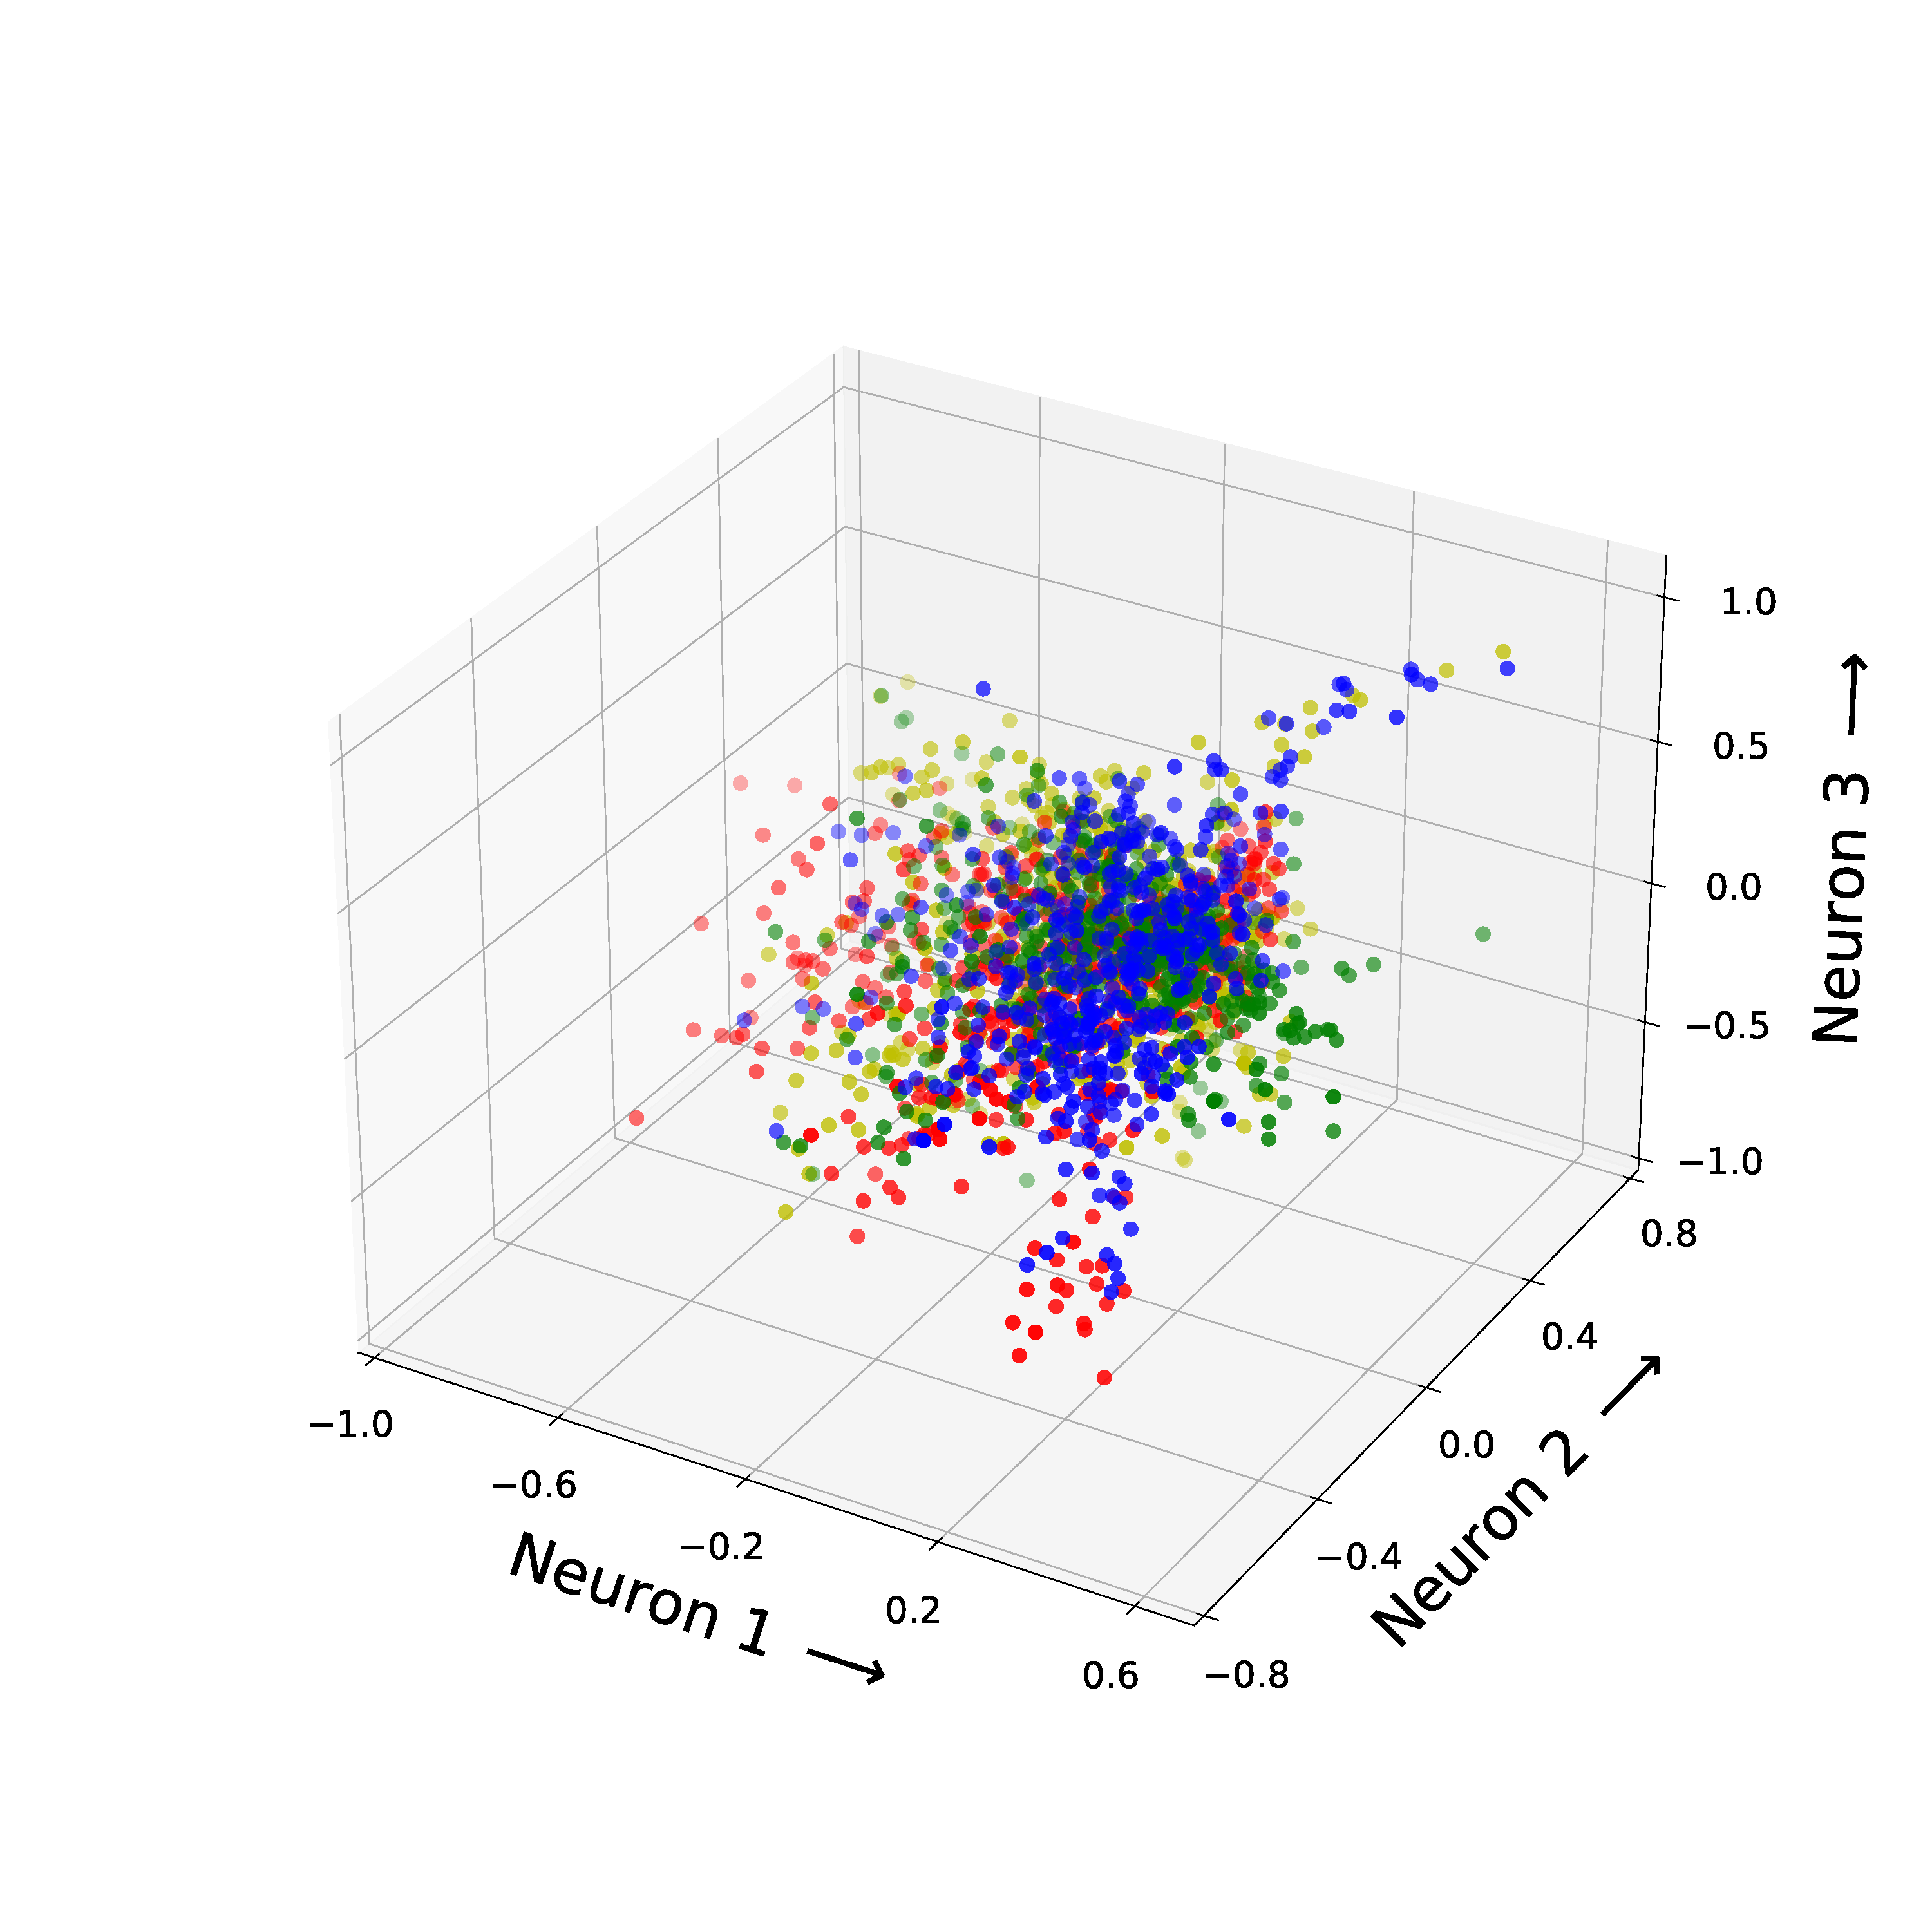
\includegraphics[width=.44\textwidth]{labeled_vs_unlabeled_point_cloud/data_distribution_labeled_mmd_0.pdf}
  \hspace{.4cm}
  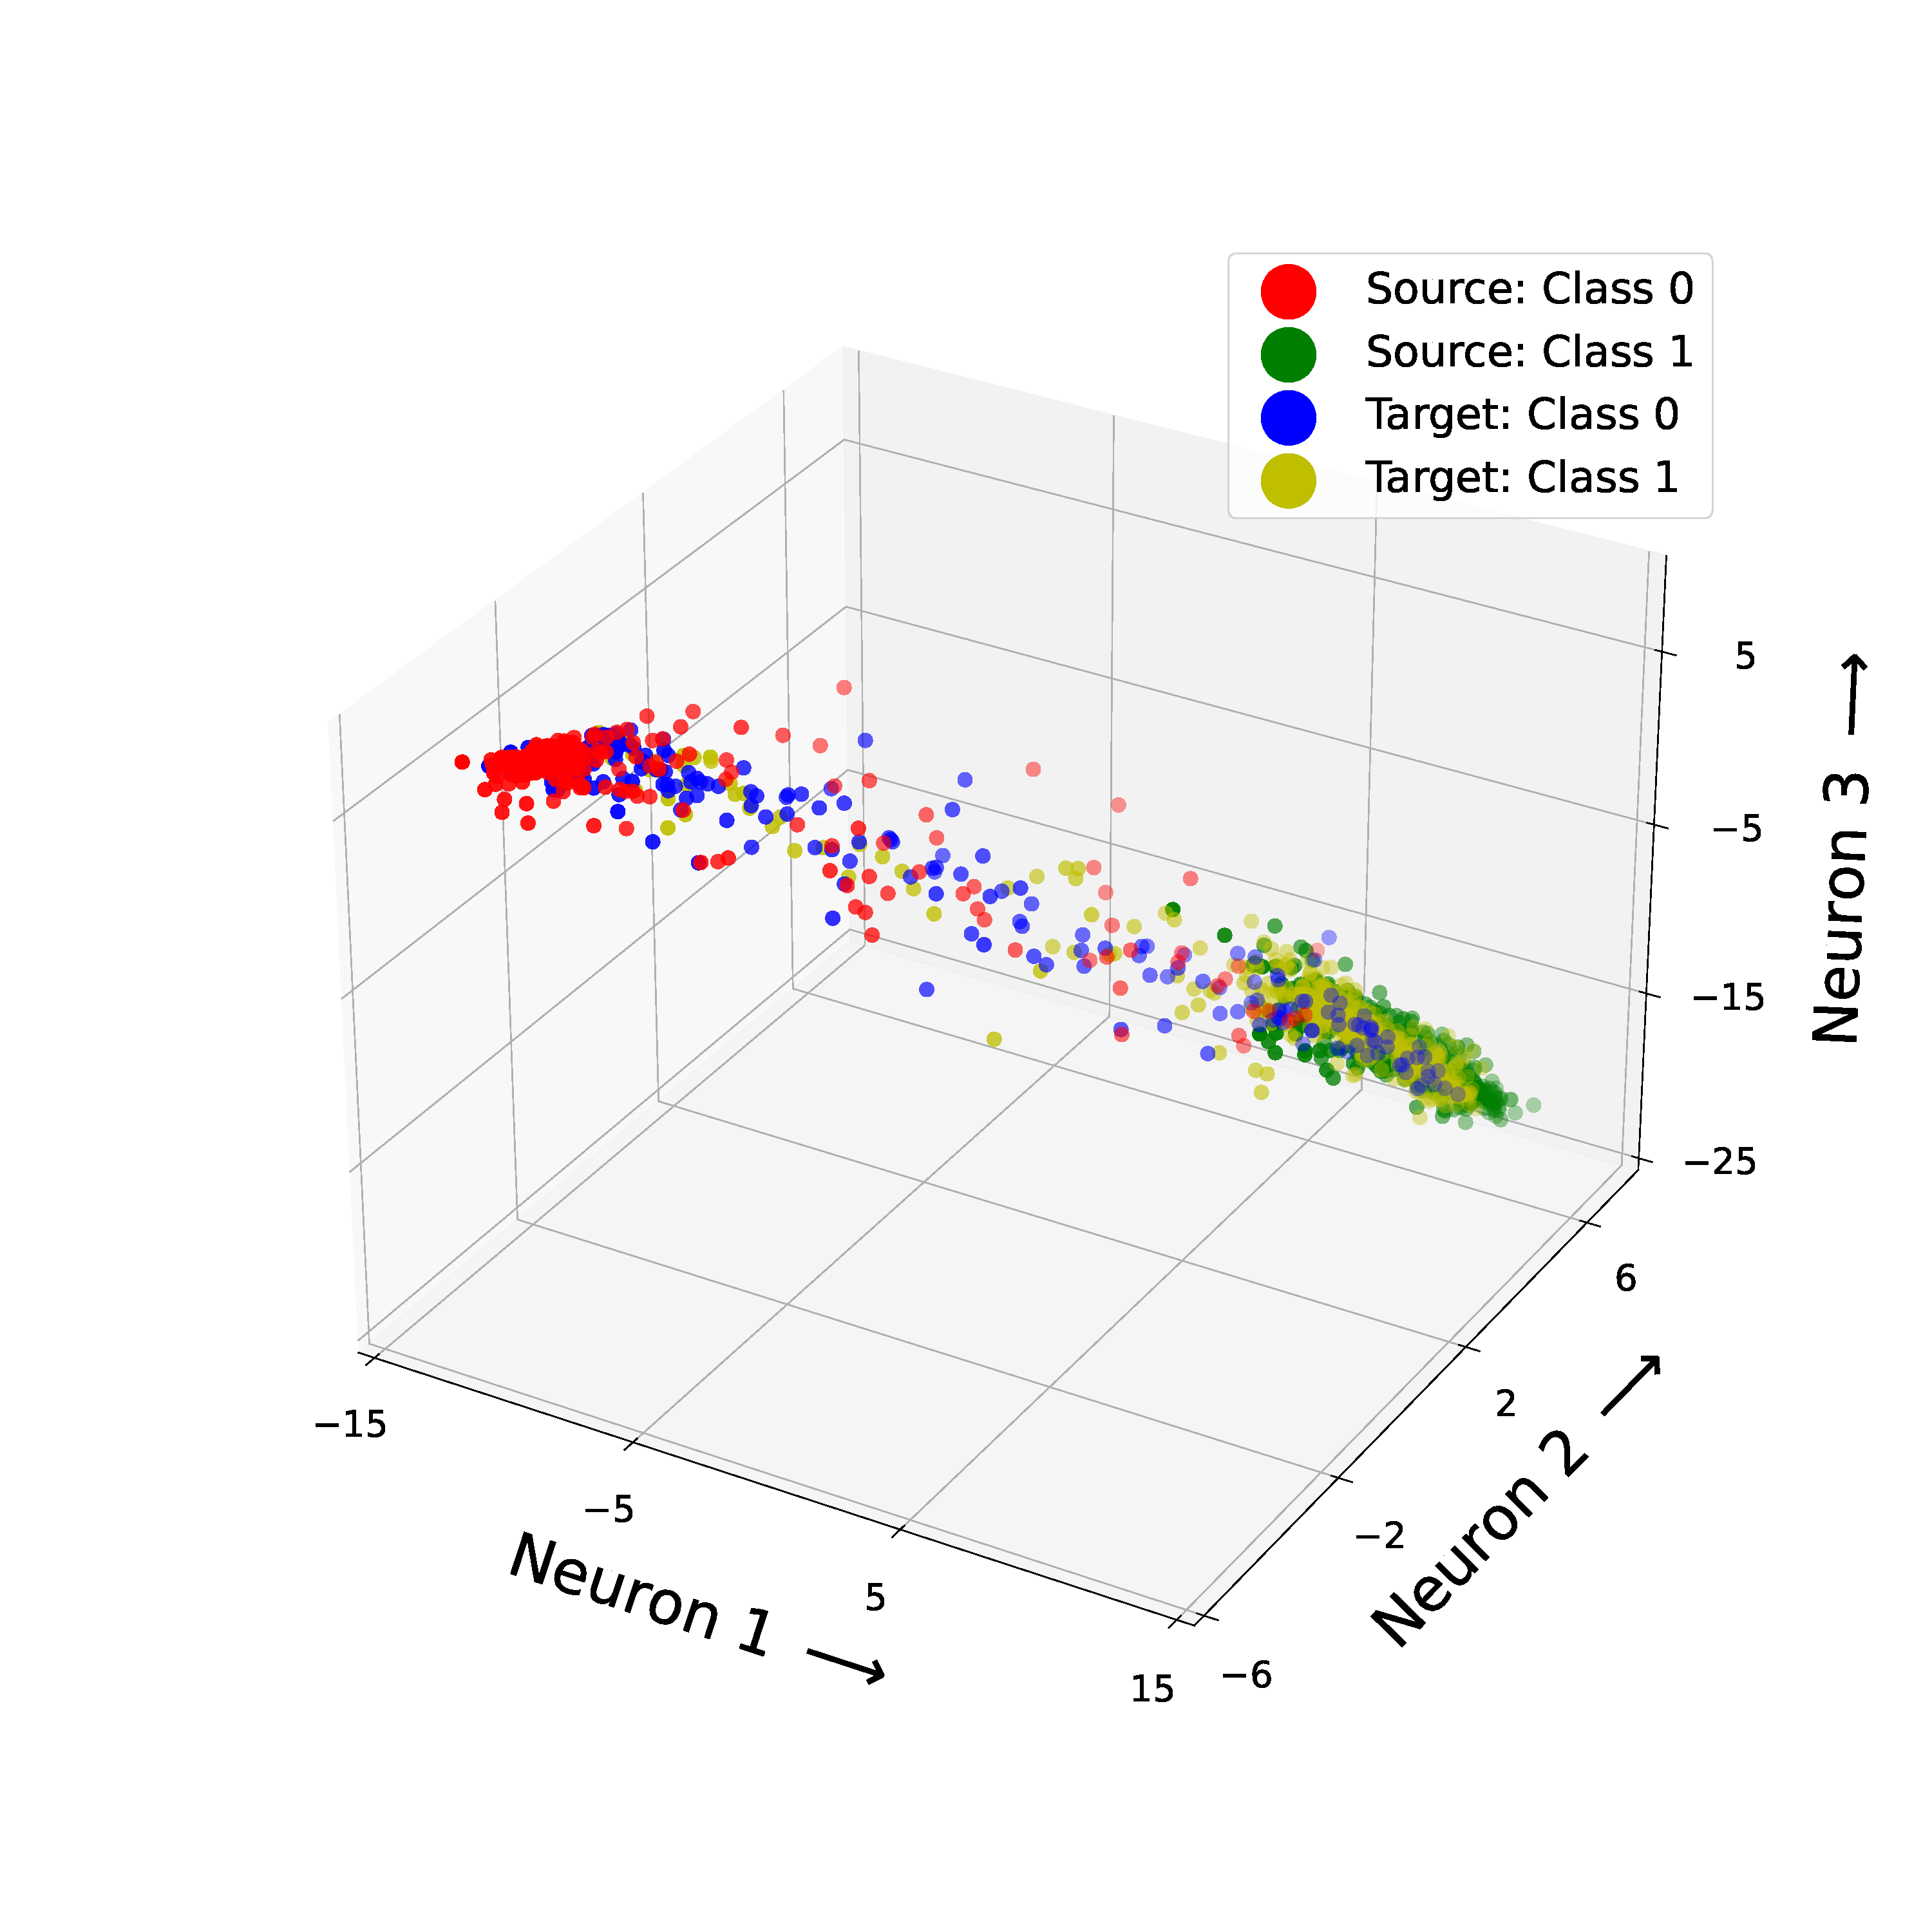
\includegraphics[width=.44\textwidth]{labeled_vs_unlabeled_point_cloud/data_distribution_labeled_mmd_8.pdf}

  \vspace{.1cm}

  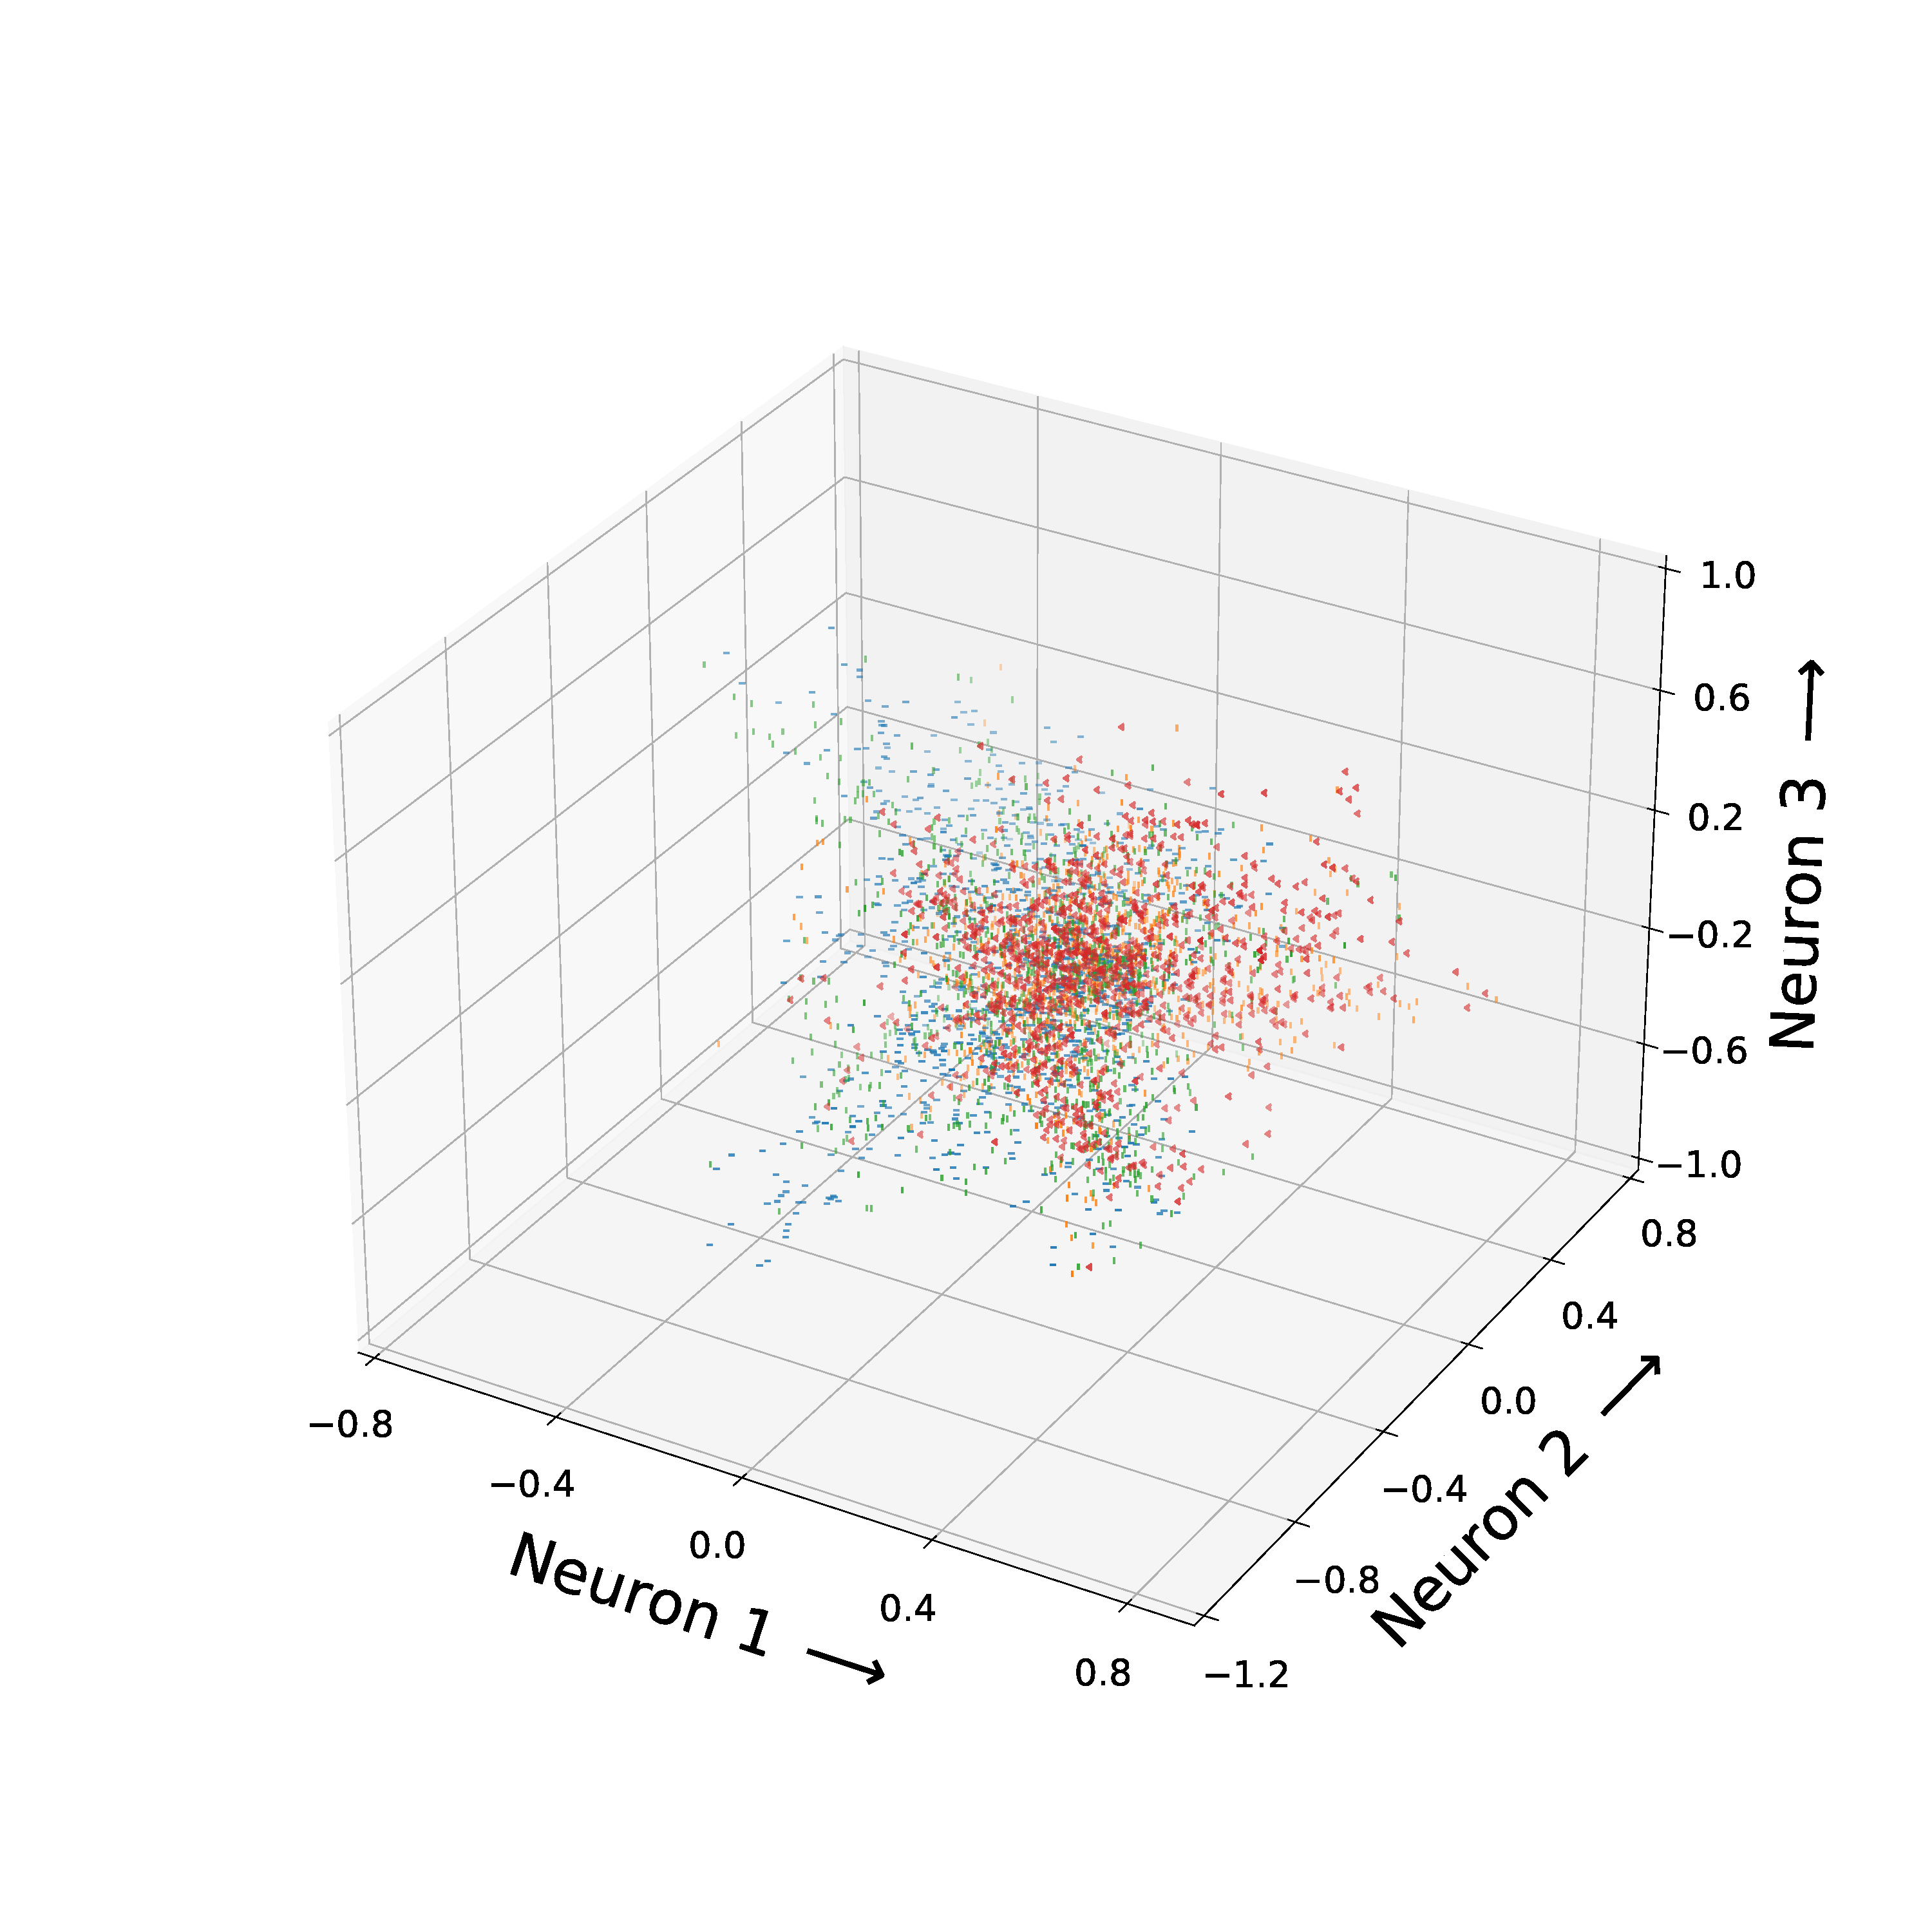
\includegraphics[width=.44\textwidth]{labeled_vs_unlabeled_point_cloud/data_distribution_regular_mmd_0.pdf}
  \hspace{.4cm}
  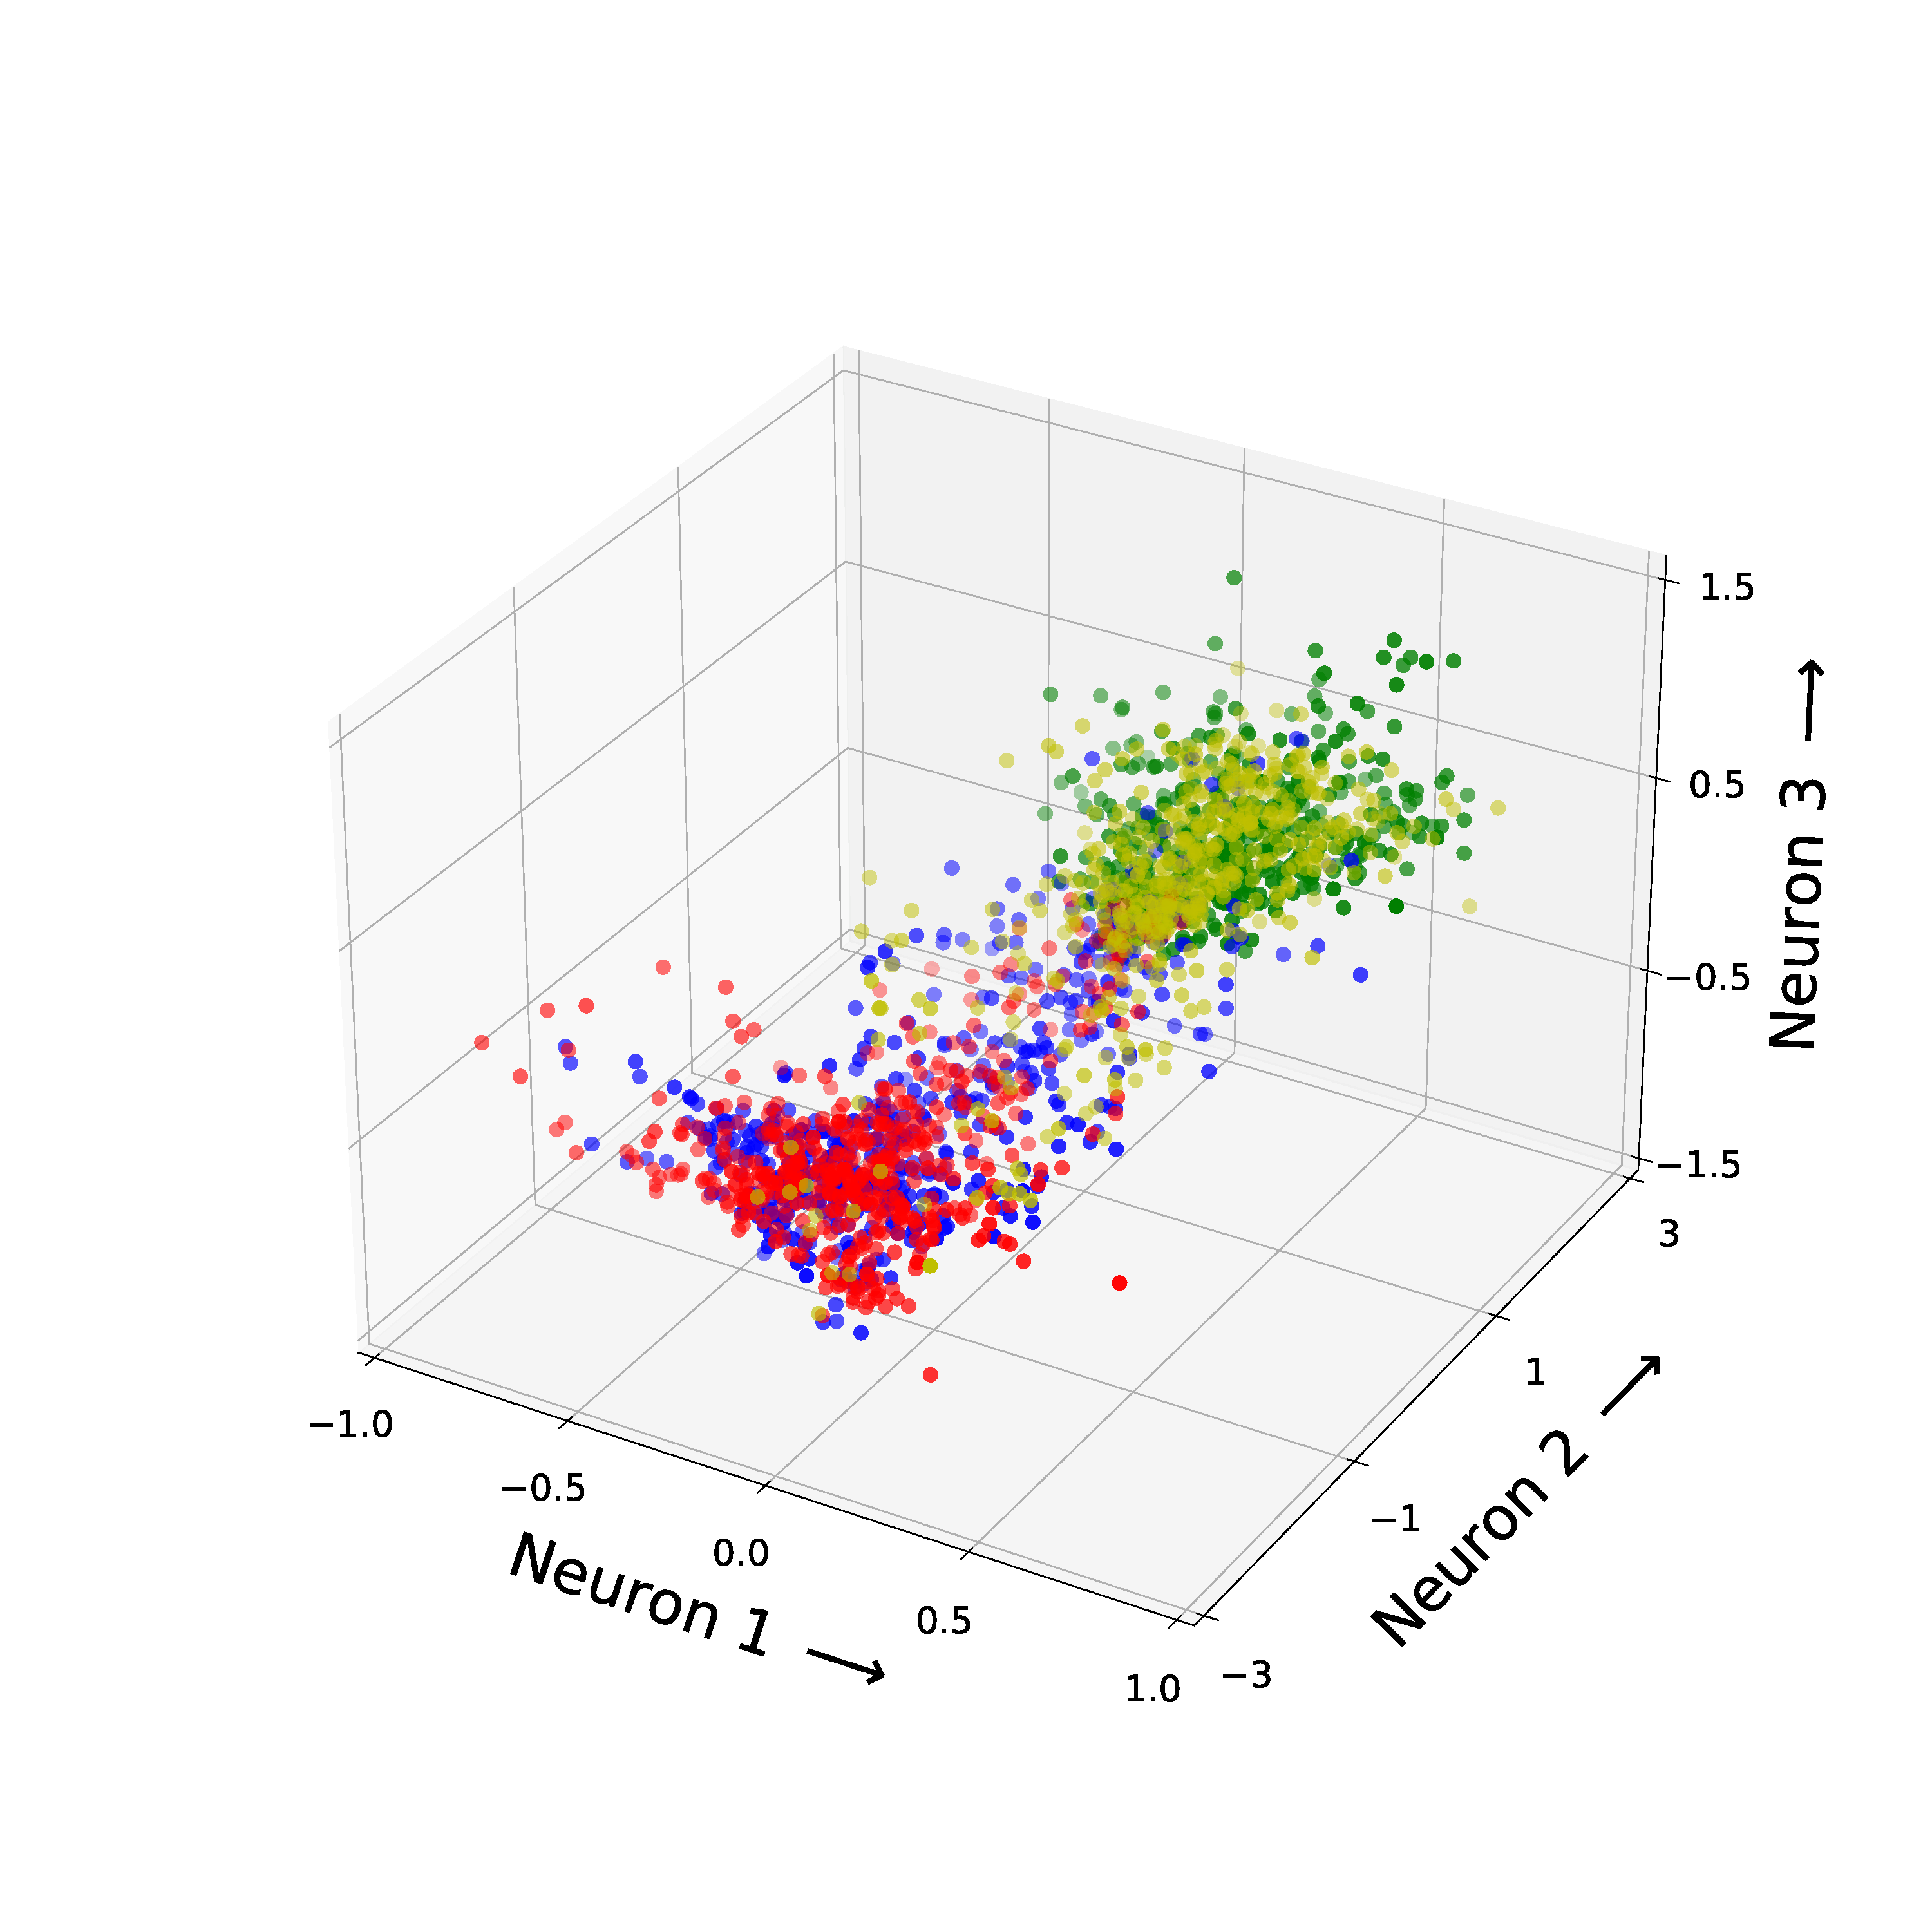
\includegraphics[width=.44\textwidth]{labeled_vs_unlabeled_point_cloud/data_distribution_regular_mmd_8.pdf}
  
  \caption{Data Distribution: Labeled MMD (top) vs. unlabeled MMD (bottom): Epoch 0 (left) vs. Epoch 8 (right)}
  \label{fig:point_cloud_labeled_unlabeled_mmd}
\end{figure}

\subsection{Influence of Latent Feature Space Choice on the Domain Adaption Performance}
\label{cnn_mmd_dummy}

This section analyzes the influence of applying the MMD-loss in different latent feature maps of the CNN and classifier. Inspired by the computer vision community especially the domain discrepancy reduction in the feature extractor layers is of great interest. Two MMD-based approaches were evaluated, which measure the domain discrepancy in different layers of the neural network. Table \ref{tab:MMD_layer_choice_dummy} specifies the used MMD-losses in more detail.

\begin {table}[H]
\centering

\begin{tabular}{llllllll}
  \toprule
  Model          & Conv1 & Conv2 & Conv3 & Flatten & FC1 & FC2 \\
  \midrule
  
 
\vspace{.5cm}

 \parbox[t]{0mm}{\multirow{1}{*}{\rotatebox[origin=c]{90}{\thead{FC \\ MMD}}}} & - & - & - & \checkmark & \checkmark & \checkmark\\
 
\vspace{.5cm}

 \parbox[t]{0mm}{\multirow{1}{*}{\rotatebox[origin=c]{90}{\thead{FULL \\ MMD}}}} & \checkmark & \checkmark & \checkmark & \checkmark & \checkmark & \checkmark\\

  \bottomrule
\end{tabular}

\caption {MMD layer choice of presented models} \label{tab:MMD_layer_choice_dummy} 
\end {table}

The development of the source and target accuracies as well as the source CE- and MMD-loss throughout the model training are visualized in fig. \ref{fig:accuracy_cnn_and_no_cnn_mmd} and fig. \ref{fig:loss_cnn_and_no_cnn_mmd}. When considering the CNN feature maps in the MMD-loss, higher source and target accuracies are achieved. Besides that, the losses, as well as the accuracies, converge faster and smoother. Reducing the domain discrepancy only in the final layers of the neural network does not sufficiently tackle the underlying reasons of the domain shift. When estimating the MMD- and CE-loss in the final layers, it seems like the two contradicting training goals work against each other. The model training seems to be less prone to local minima, which leads to instabilities. The corresponding fluctuations can be seen in the training curves. The model performance sometimes breaks down after some stable epochs of constant training. Anyhow, one has to remember calculating the regular FULL MMD-loss is quite expansive since the feature maps of the convolutional layers are complex and high-dimensional.

\begin{figure}[htp]
  \centering
  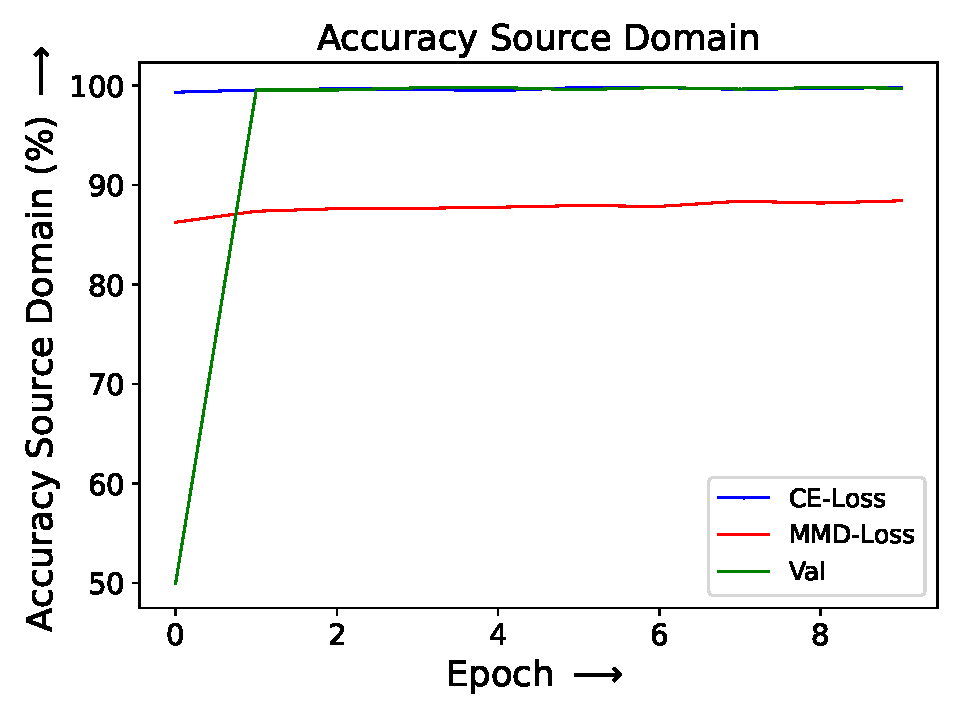
\includegraphics[width=.47\textwidth]{plots_CNN_MMD/Accuracy_Source_Domain_CNN_MMD.pdf}
  \hspace{.3cm}
  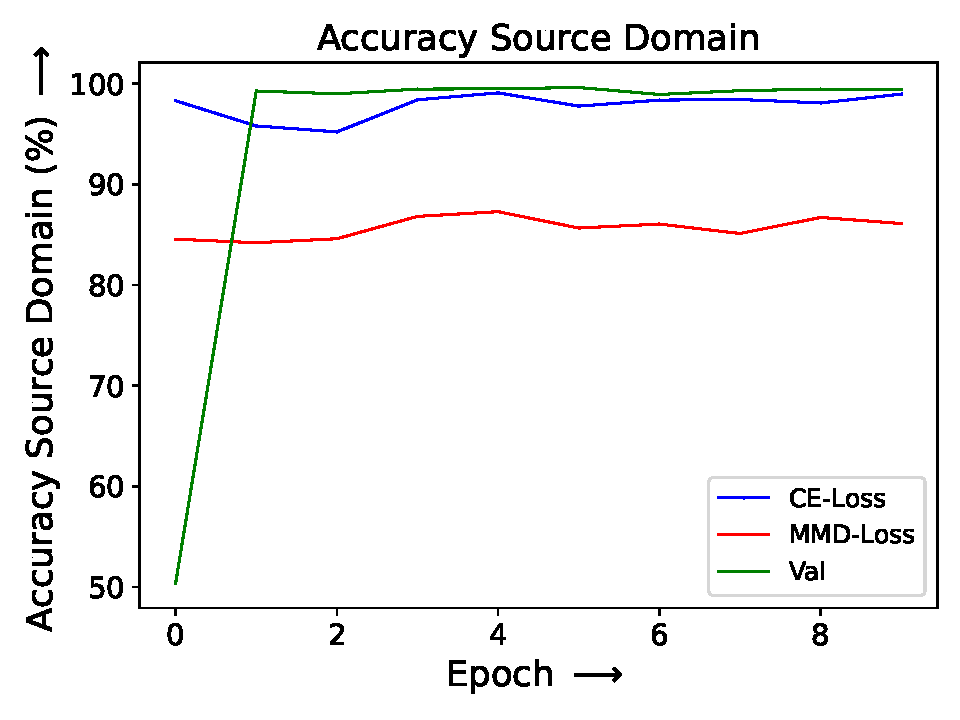
\includegraphics[width=.47\textwidth]{plots_CNN_MMD/Accuracy_Source_Domain_FC_MMD.pdf}

  \vspace{.1cm}

  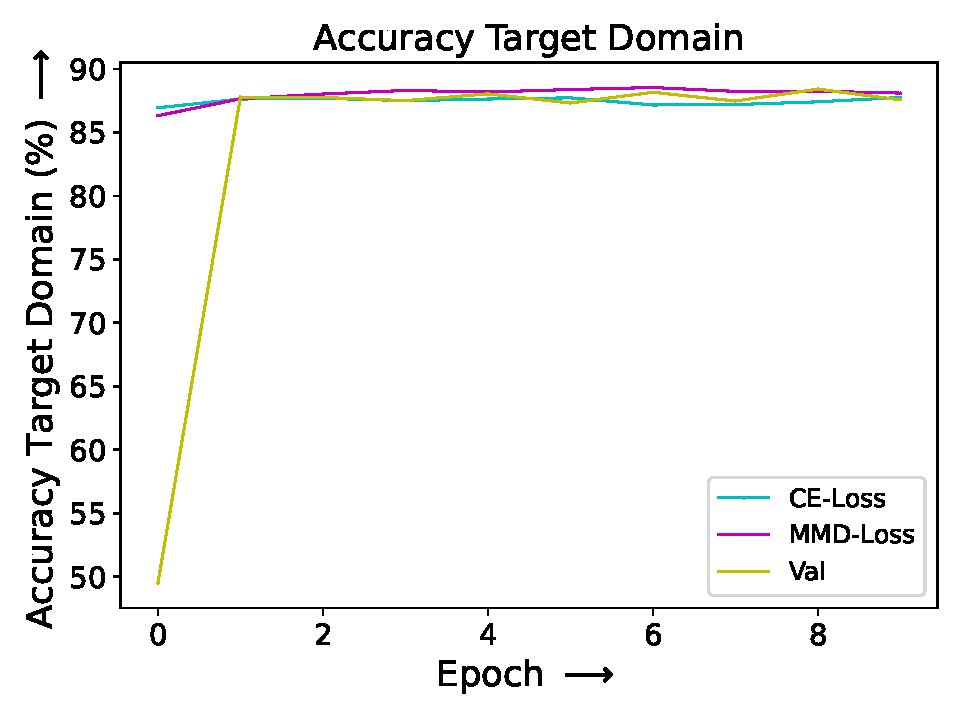
\includegraphics[width=.47\textwidth]{plots_CNN_MMD/Accuracy_Target_Domain_CNN_MMD.pdf}
  \hspace{.3cm}
  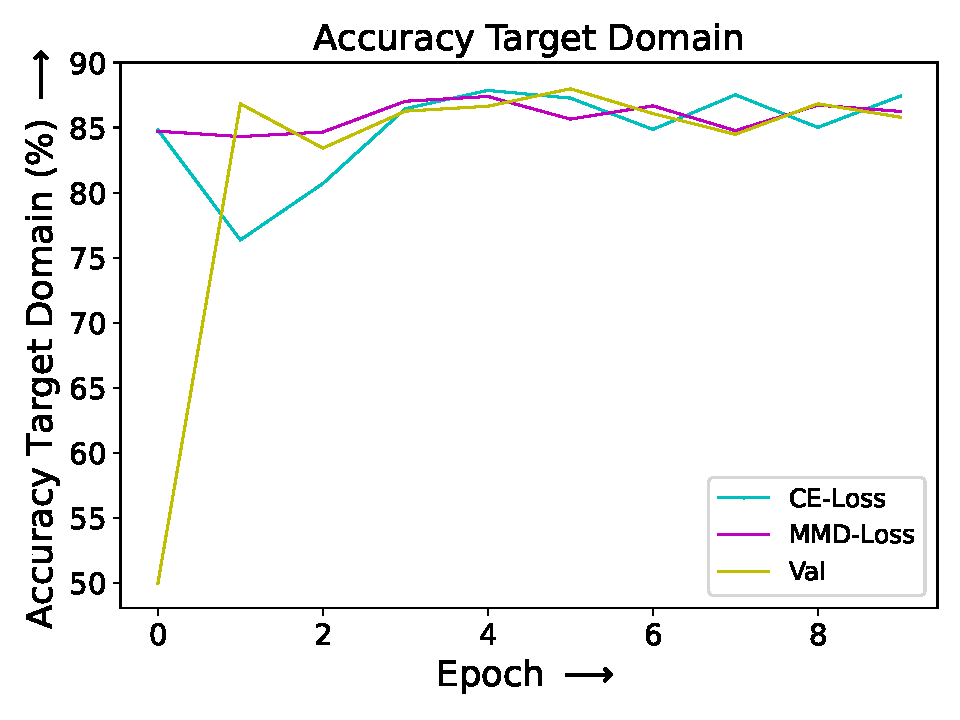
\includegraphics[width=.47\textwidth]{plots_CNN_MMD/Accuracy_Target_Domain_FC_MMD.pdf}

  \caption{Source and Target Accuracy: MMD in CNN (left), MMD in FC (right)}
  \label{fig:accuracy_cnn_and_no_cnn_mmd}
\end{figure}

\begin{figure}[H]
  \centering
  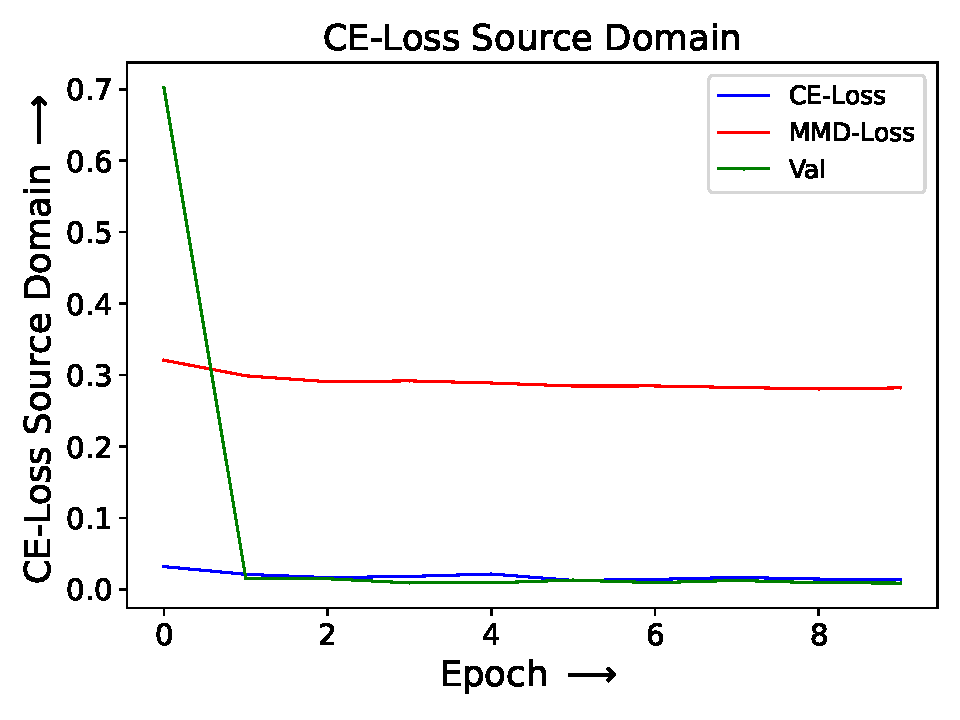
\includegraphics[width=.47\textwidth]{plots_CNN_MMD/CE_Loss_Source_Domain_CNN_MMD.pdf}
  \hspace{.3cm}
  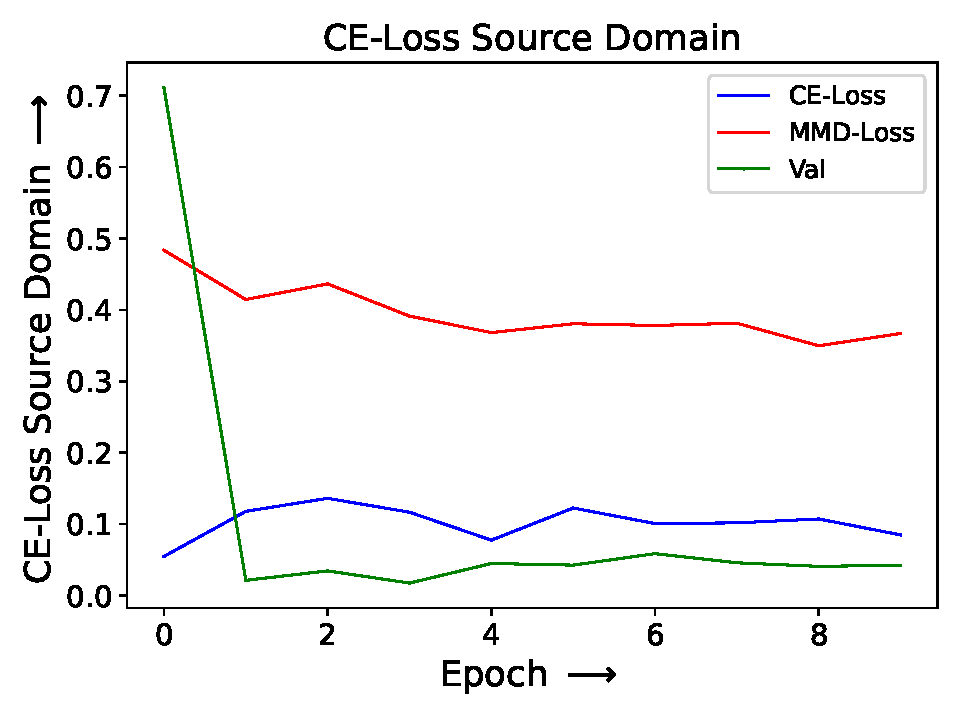
\includegraphics[width=.47\textwidth]{plots_CNN_MMD/CE_Loss_Source_Domain_FC_MMD.pdf}

  \vspace{.1cm}

  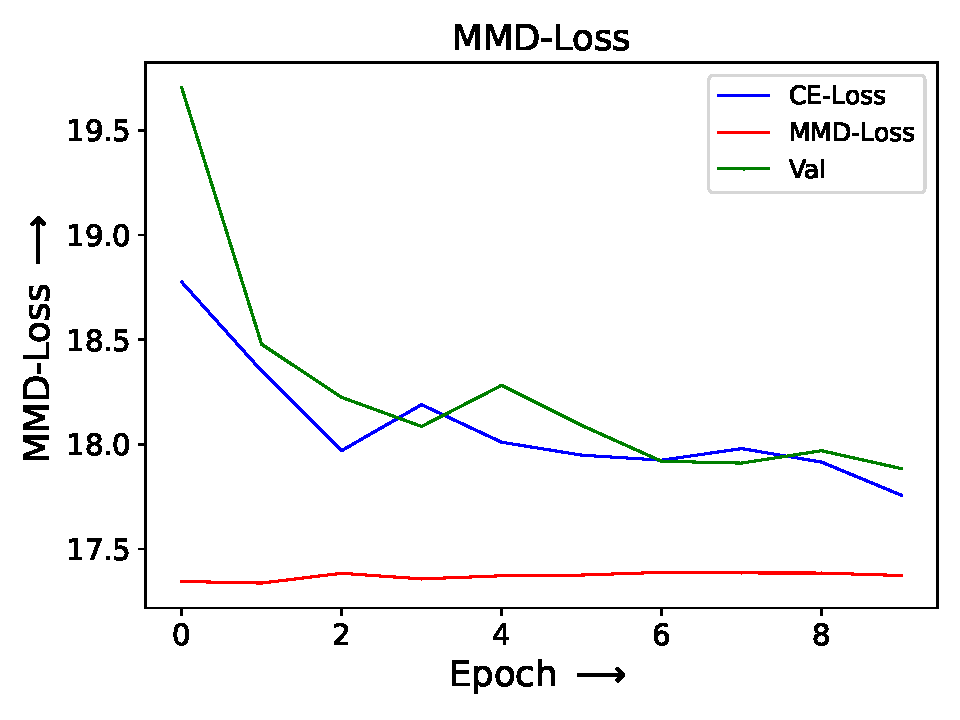
\includegraphics[width=.47\textwidth]{plots_CNN_MMD/MMD_Loss_CNN_MMD.pdf}
  \hspace{.1cm}
  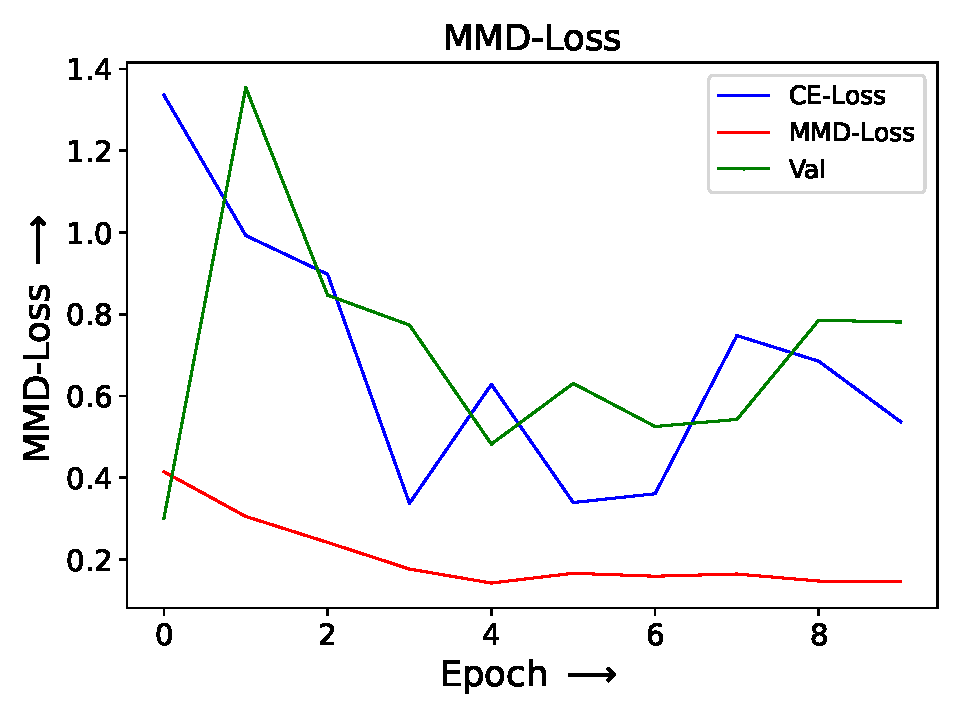
\includegraphics[width=.48\textwidth]{plots_CNN_MMD/MMD_Loss_FC_MMD.pdf}

  \caption{MMD- and CE-Loss: MMD in CNN (left), MMD in FC (right)}
  \label{fig:loss_cnn_and_no_cnn_mmd}
\end{figure}

\section{Real-World Dataset}
In the following section the performance of different MMD-based domain adaption models are evaluated on the real-world BSD dataset. The goal of this chapter is to evaluate the benefits and problems of the presented approach for PHM on industrial machines. All presented models have the same architecture and optimization strategies but differ in the applied MMD-loss. Different GAMMA and MMD layer choices were evaluated. The performance of each model is compared with the baseline model, which does not use any MMD-loss during training. The following table specifies the latent feature spaces included in the different applied MMD-losses:

\begin {table}[H]
\centering

\begin{tabular}{llllllll}
  \toprule
  Model          & Conv1 & Conv2 & Conv3 & Flatten & FC1 & FC2 \\
  \midrule
  
\vspace{.5cm}

 \parbox[t]{0mm}{\multirow{1}{*}{\rotatebox[origin=c]{90}{\thead{BASE- \\ LINE}}}} & - & - & - & - & - & -\\
 
\vspace{.5cm}

 \parbox[t]{0mm}{\multirow{1}{*}{\rotatebox[origin=c]{90}{\thead{FULL \\ MMD}}}} & \checkmark & \checkmark & - & \checkmark & \checkmark & \checkmark\\
 
\vspace{.5cm}

 \parbox[t]{0mm}{\multirow{1}{*}{\rotatebox[origin=c]{90}{\thead{FC \\ MMD}}}} & - & - & - & \checkmark & \checkmark & \checkmark\\
 
\vspace{.5cm}

 \parbox[t]{0mm}{\multirow{1}{*}{\rotatebox[origin=c]{90}{\thead{CNN \\ MMD}}}} & \checkmark & \checkmark & \checkmark & - & - & -\\

 
  \bottomrule
\end{tabular}

\caption {MMD layer choice of presented models} \label{tab:MMD_layer_choice} 
\end {table}

Similarly to the dummy dataset, the influence of GAMMA and the MMD layer choice on the PHM performance are examined in the chapter \ref{ch:Influence_GAMMA_real_dataset} and \ref{ch:Influence_Layer_real_dataset}. Since the previously presented labeled MMD-loss uses target labels, which all other models do not, it was not included in the evaluation on the real-world data. To achieve good comparability just models with equal training conditions and data access are considered. The labeled MMD-loss is interesting in a research aspect, since it reveals the deficits of the unlabeled MMD-loss. Anyhow, these methods are impractical for the real-world use. In domain adaption approaches, neural networks are first trained on the source domain and afterwards transferred to the target domain. If that optimization process requires target labels, one could train the neural network directly on the target domain. Besides that, these approaches expect the labeling of the target domain data, which can be quite time consuming. The necessity of target labels prevents the easy adaption of models, trained on the source domain data, to various tasks by solely including the corresponding unlabeled target dataset. Besides that, the labeled MMD loss expects additional hyperparameters. Tuning the labeled MMD-loss is more complicated and expects further experiments to find appropriate hyperparameters. Also, due to the limited time in the thesis the focus of the investigations on the real-world dataset lies in the regular MMD-loss. In chapter \ref{ch:PHM_performance} the performance of these models are compared based of their target domain test accuracy. For the implementation of the presented models, PyTorch was used. All computations were performed on a Leibniz Supercomputing Centre7 compute node virtual machine with 20
Intel® Xeon® Gold 6148 vCPUs, one Nvidia® Tesla V100, 368 GB RAM, PyTorch v.1.4.0 and CUDA 10.1.


\begin{comment}
In the following section the performance of different MMD-based domain adaption approaches are evaluated on the real-world ball screw drive dataset. The model used for this evaluation is presented in fig. \ref{fig:model_real_data}. From the 49 features in the dataset just three (\verb|'C:x_bottom'|, \verb|'C:y_bottom'|, \verb|'C:z_bottom'|) are used. For this reasons three sequences of length 1024 are fed into the CNN.

\begin{figure}[H]
  \centering
  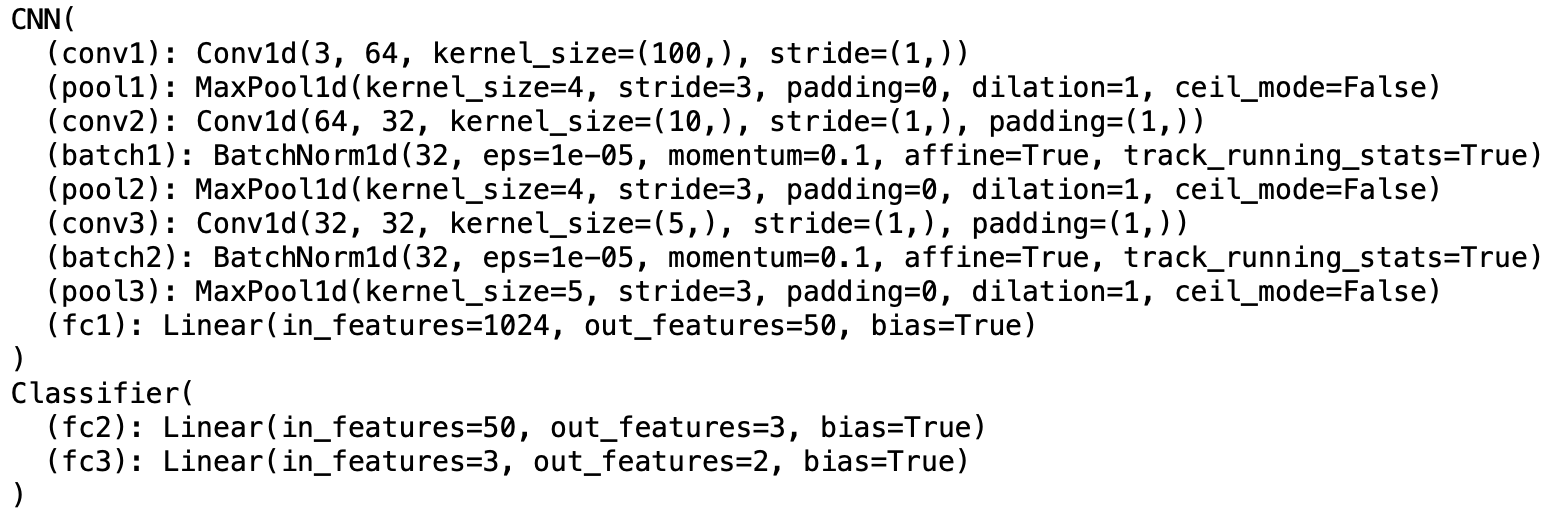
\includegraphics[width=1.1\textwidth]{model_real_data}
  \caption {MMD Model for Real Dataset} \label{fig:model_real_data}
\end{figure}


On the real machine dataset the three approaches regular FC + CNN MMD-loss,  regular FC MMD and no MMD-loss are evaluated. The accuracies on the source and target domain are visualized in fig. \ref{fig:accuracy_real_world}. In each figure three curves are presented representing different phases of the training. During the MMD-loss phase the whole model consisting of CNN and classifier are optimized with a weighted average of MMD and CE loss. In the CE-loss phase just the classifier is optimized according to a CE-loss. During both phases an ADAM optimizer with a learning rate of 1e-2, beta1 of 0.9 and beta2 of 0.99 is used . In the val phase the model is evaluated. Before the training the data is split for these three phases accordingly (MMD-loss: 60\%, CE-loss: 20\%, Val: 20\%). Therefore all experiments follow a proper train validation split. It becomes obvious that the accuracies achieved on the validation set of the target domain were able to be increased with about 10\% by using the two MMD variations. The MMD and CE-loss seems to be decreased more smoothly when including CNN features into the MMD-loss for the optimization of the model. Also the accuracy achieved on the target validation set achieved the regular FC + CNN MMD-loss beat the one achieved with the regular FC MMD-loss. Without using any MMD-loss the model performance on the target domain could be increased by just around 2\%. When using the regular FC MMD-loss sometimes the performance of the model breaks down  little bit. Often times this can be seen in the accuracy of the target and source domain. An example for this phenomena can be seen in fig. \ref{fig:accuracy_real_world} when looking at the accuracies of regular FC MMD (middle). In epoch ~27 the accuracy breaks down on the target and source domain. Especially during the combined training with the MMD and CE loss this effect becomes especially obvious. Like mentioned in previous chapters this shows that when not including the latent features of the CNN in the MMD-loss the CE and MMD-loss seem to work against each other, which makes the optimization less stable.

\begin{figure}[H]
  \centering
  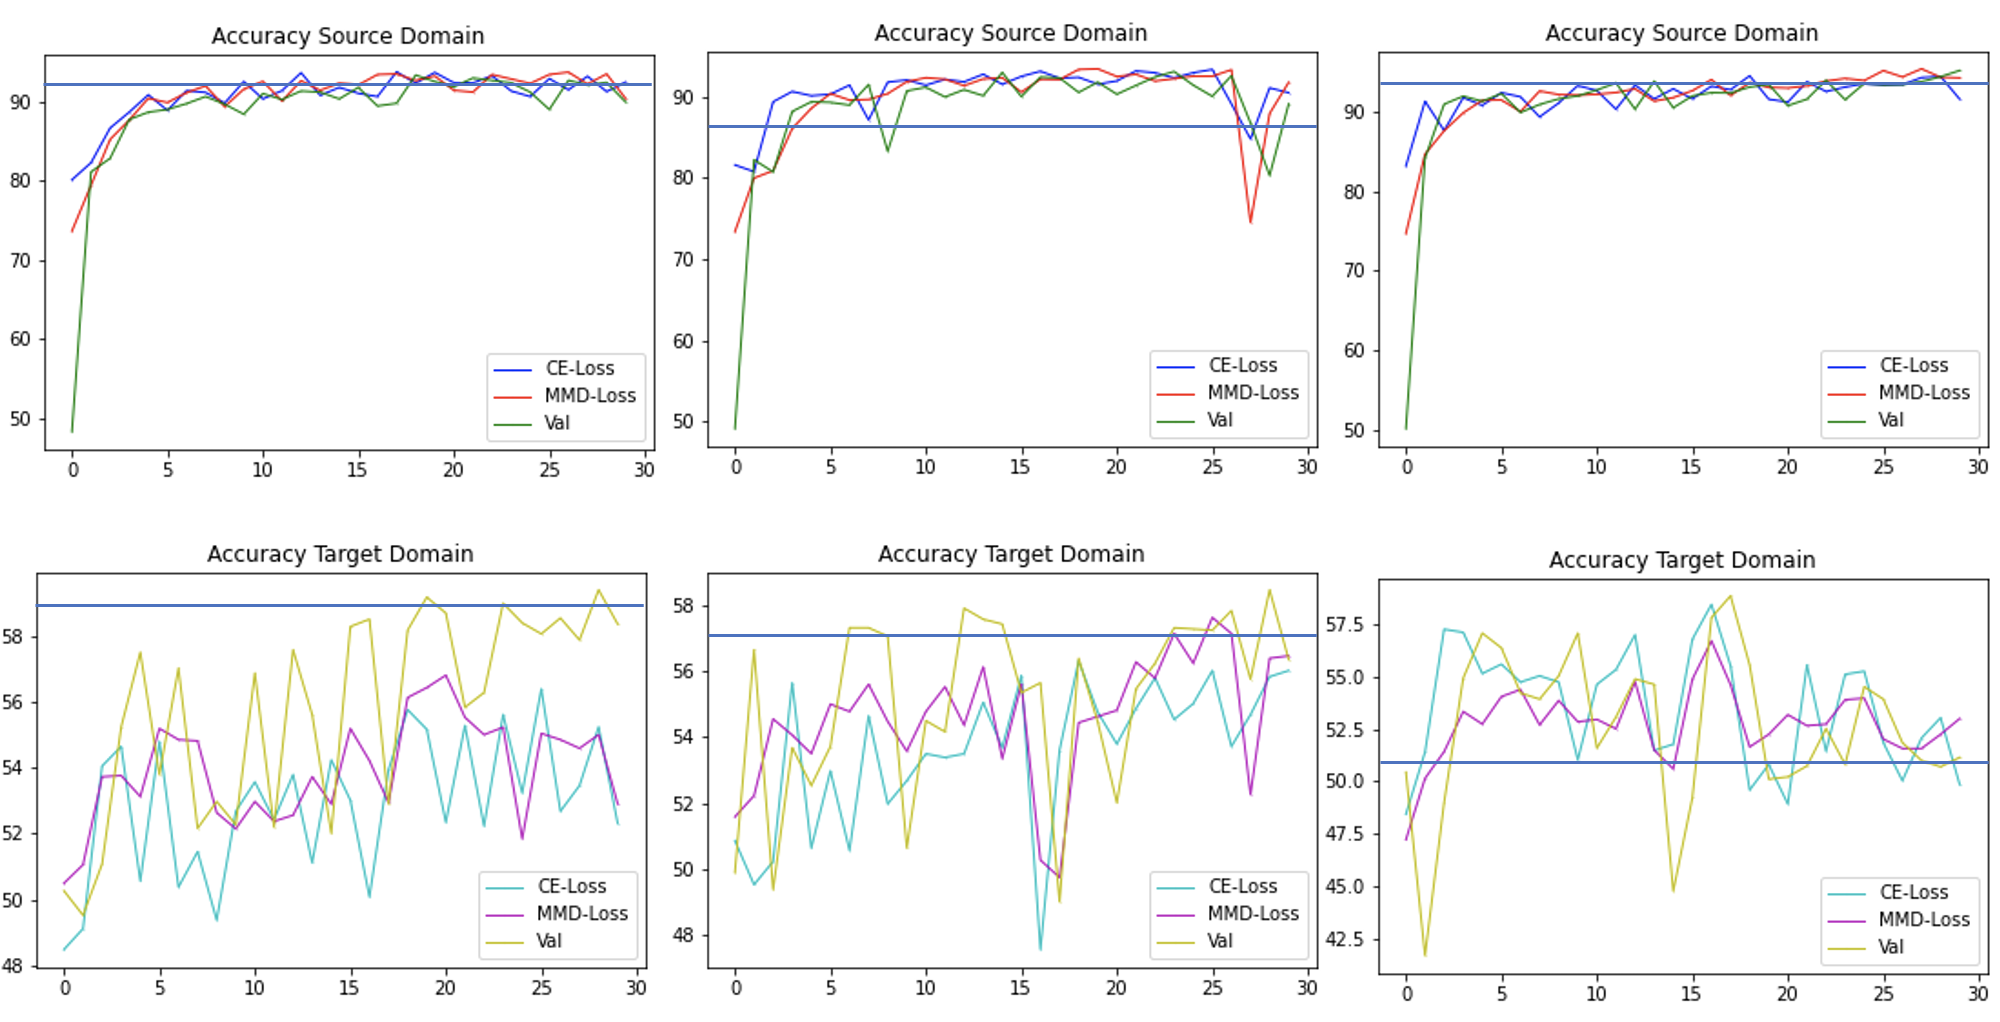
\includegraphics[width=1.1\textwidth]{accuracy_real_world}
  \caption {Source and Target Accuracies for model training with Regular FC + CNN MMD-loss (left), Regular FC MMD (middle) and No MMD-loss (right)} \label{fig:accuracy_real_world}
\end{figure}


\begin{figure}[H]
  \centering
  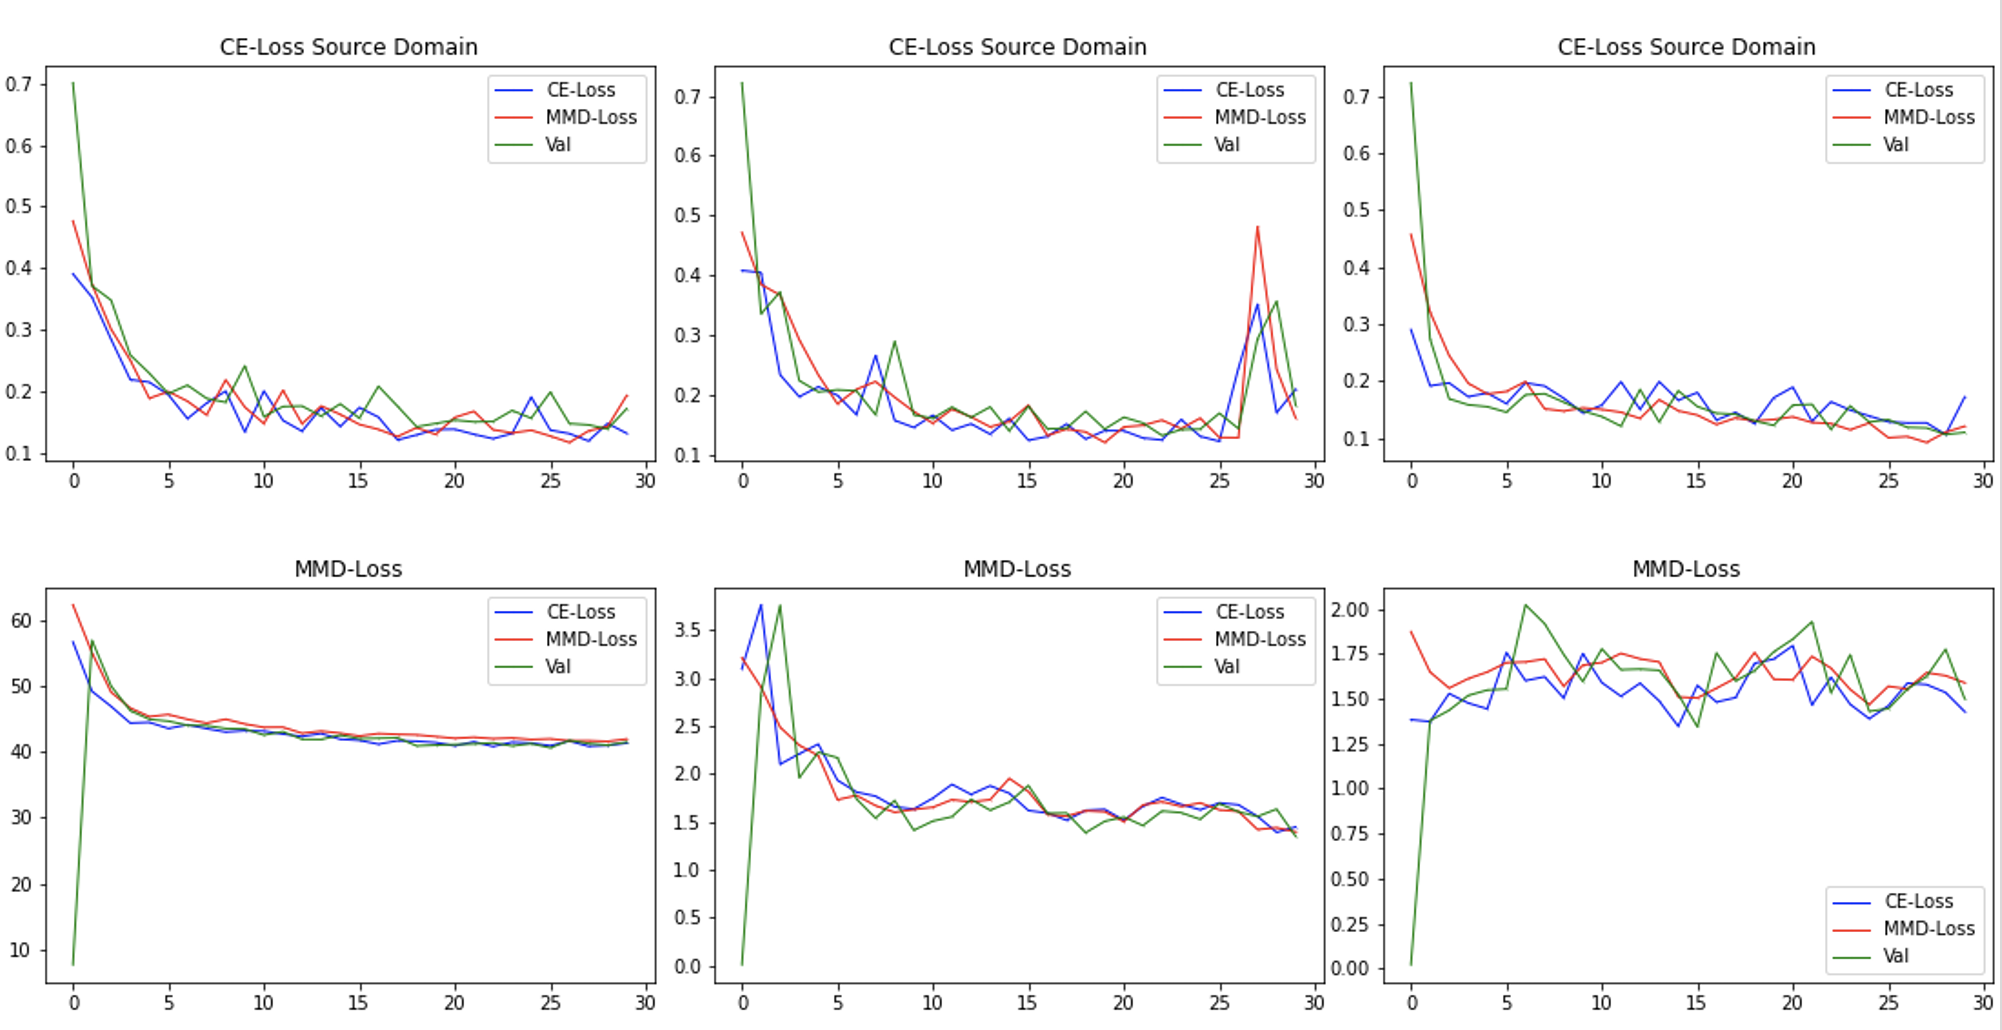
\includegraphics[width=1.1\textwidth]{loss_real_world}
  \caption {Loss for model training with Regular FC + CNN MMD-loss (left), Regular FC MMD (middle) and No MMD loss} \label{fig:loss_real_world}
\end{figure}


In fig. the development of the source CE and MMD-loss is shown. It can be seen, that the hyperparameter GAMMA was picked well, such that the MMD as well as the source CE-loss were able to be reduced smoothly throughout the trainings process. 


Unfortunately the MMD-loss could just minimize the domain discrepancy by a little. The domain discrepancy problem couldn't be solved completely. Still the idea of the MMD-loss becomes more clear in the experiments. Also the positive effect of the MMD-loss for the training is obvious. For the complex multi-dimensional dataset the MMD-loss is probably not sophisticated enough to detect and effectively fight the domain discrepancy.
\end{comment}

\subsection{Influence of GAMMA Choice on the PHM Performance}\label{ch:Influence_GAMMA_real_dataset}

In the following three models are trained with a FULL MMD-loss and different GAMMAs (0.05, 0.4, 20). For the experiments the models were trained on the  D:P mech./X signal for 100 epochs. Similarly to the dummy dataset, the model training is very sensitive to the GAMMA choice. Just when GAMMA is chosen carefully, the source CE- and MMD-loss can be reduced simultaneously. In this case the domain discrepancy in the hidden layers can be reduced while improving the prediction accuracy on the source domain data. Fig. \ref{fig:distribution_GAMMA_influence_real_data} shows the latent feature representation of the source and target domain samples in FC2. The left column shows the data distribution at epoch 0 and the right one at epoch 100. Applying the MMD-loss with a GAMMA of 0.05 increases the compactness and therefore the overlap of the classes in both domains. From the plots it is hard to make a statement about the separability of the classes. For a GAMMA of 0.05, the structure of the data distribution seems to be clearer and smoother. This rises the assumption, that separating the classes in this scenario is easier. When choosing a GAMMA of 1 the MMD-loss becomes too dominant. Noise and unimportant information are transferred between the domains. This destroys the structure of the source and target domain data, which makes the classification task impossible. In this case the feature representations of all samples collapse at a small latent feature subspace.

\begin{figure}[htp]
  \centering
  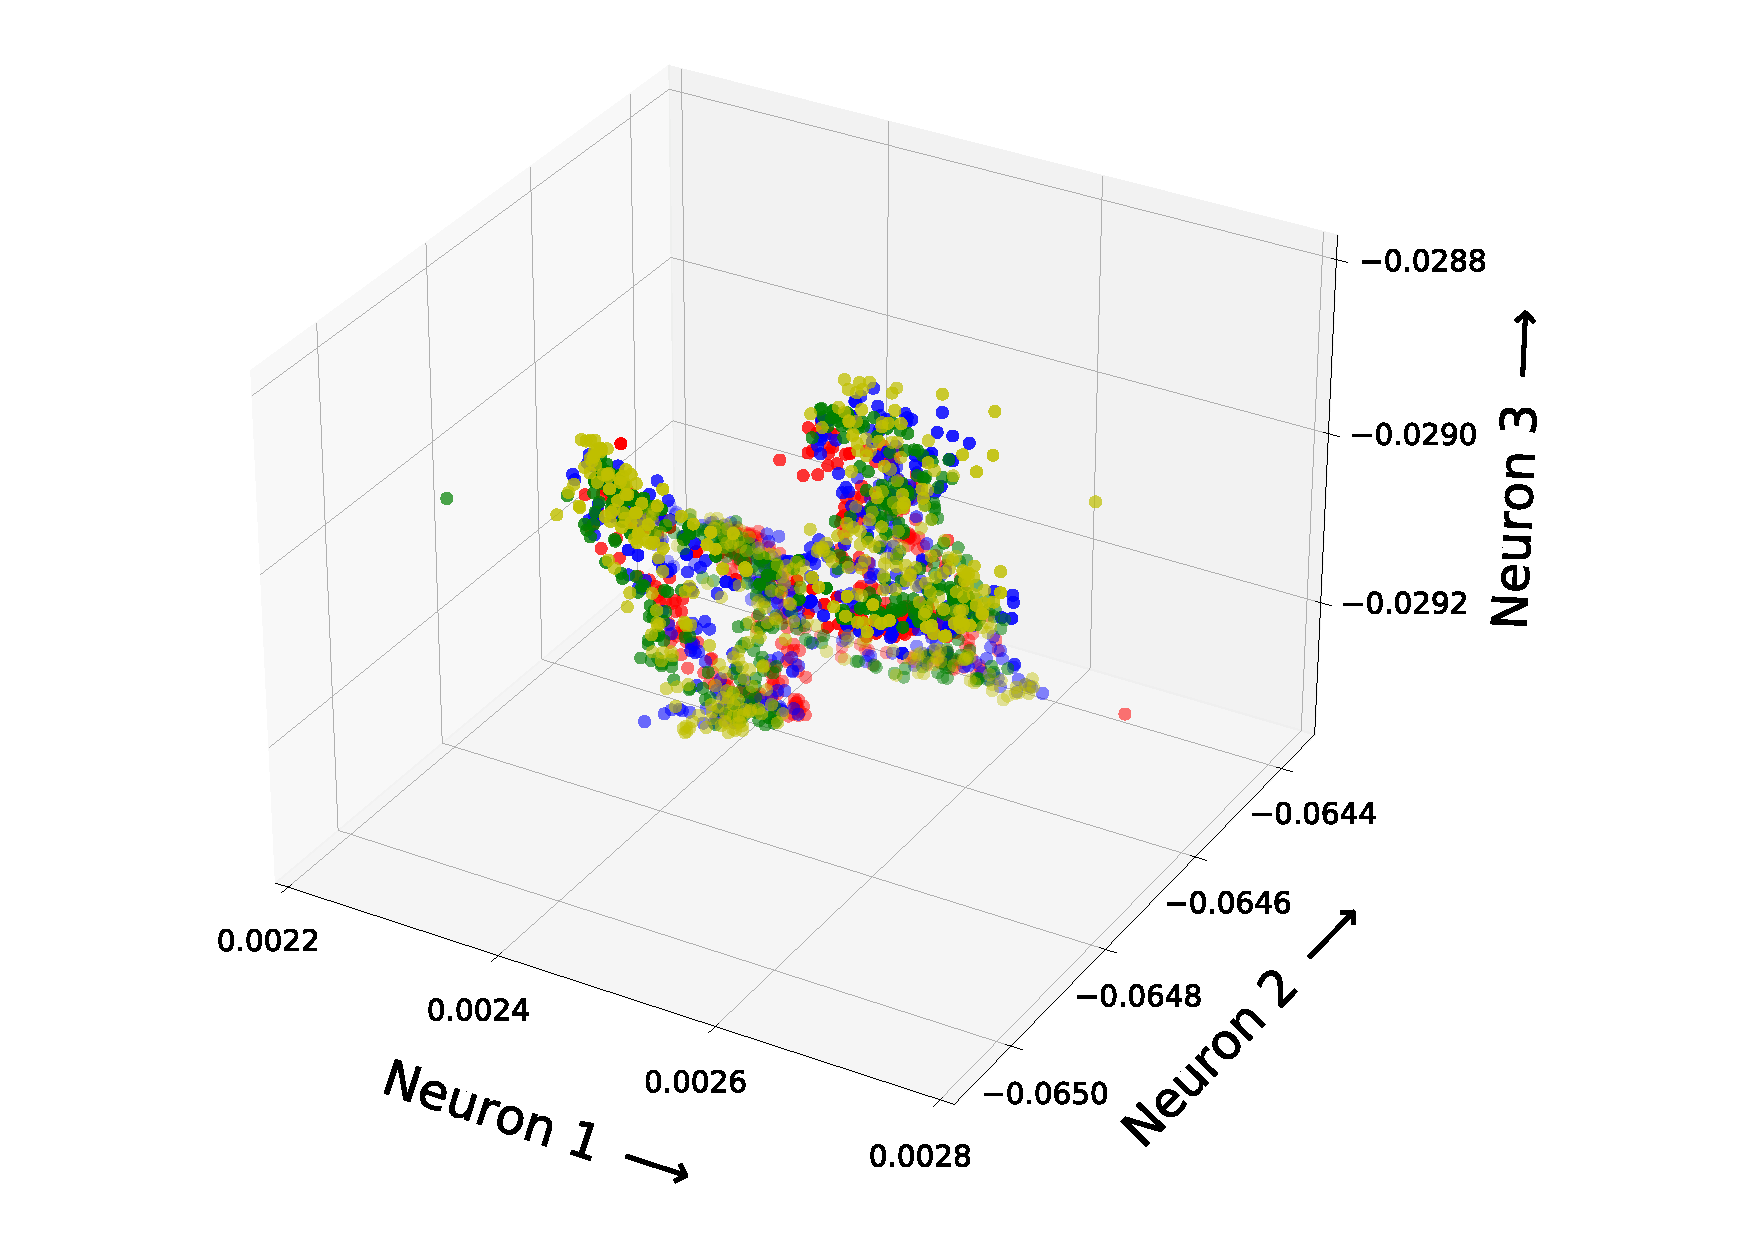
\includegraphics[width=.47\textwidth]{GAMMA_Influence_real_data/P_mech_X_data_distribution_0_GAMMA_0_0.pdf}
  \hspace{.4cm}
  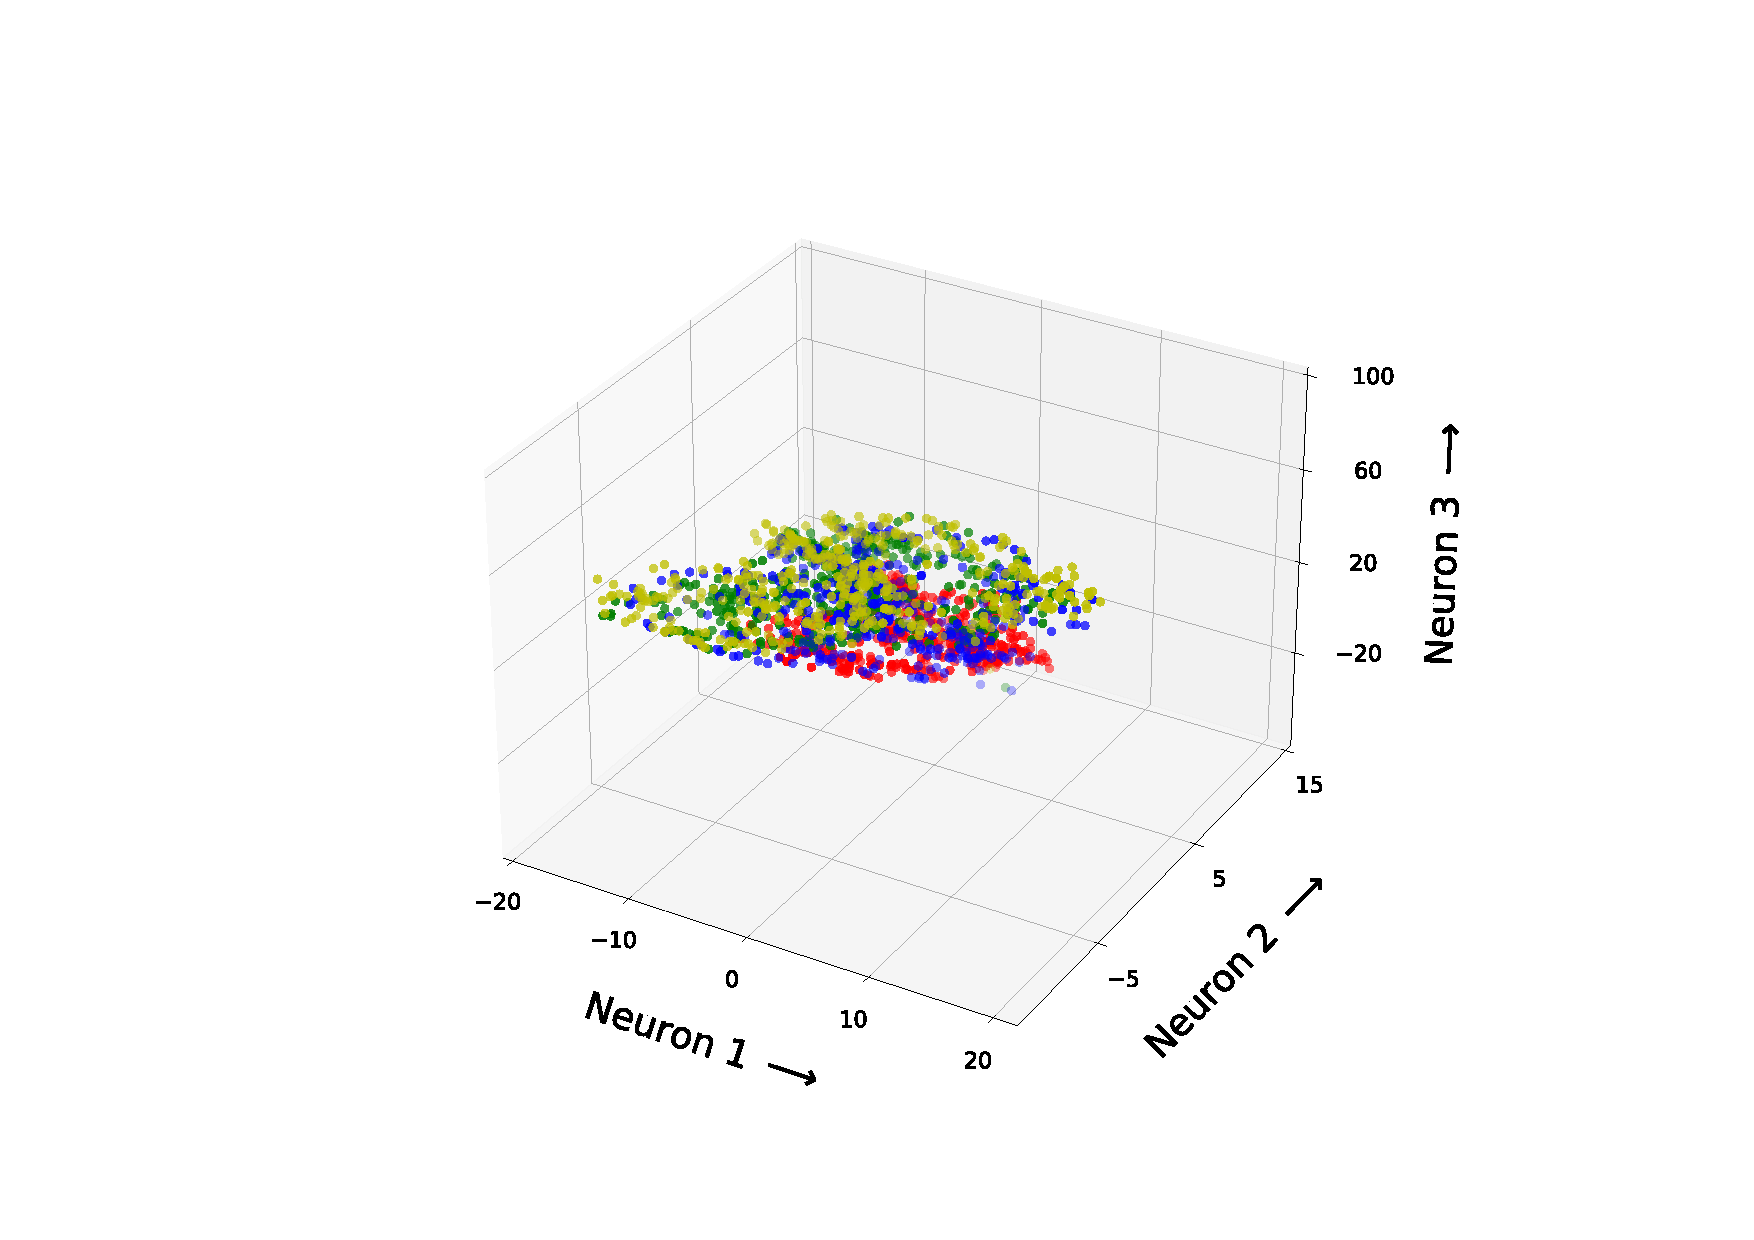
\includegraphics[width=.47\textwidth]{GAMMA_Influence_real_data/P_mech_X_data_distribution_80_GAMMA_0_0.pdf}

  \vspace{.1cm}

  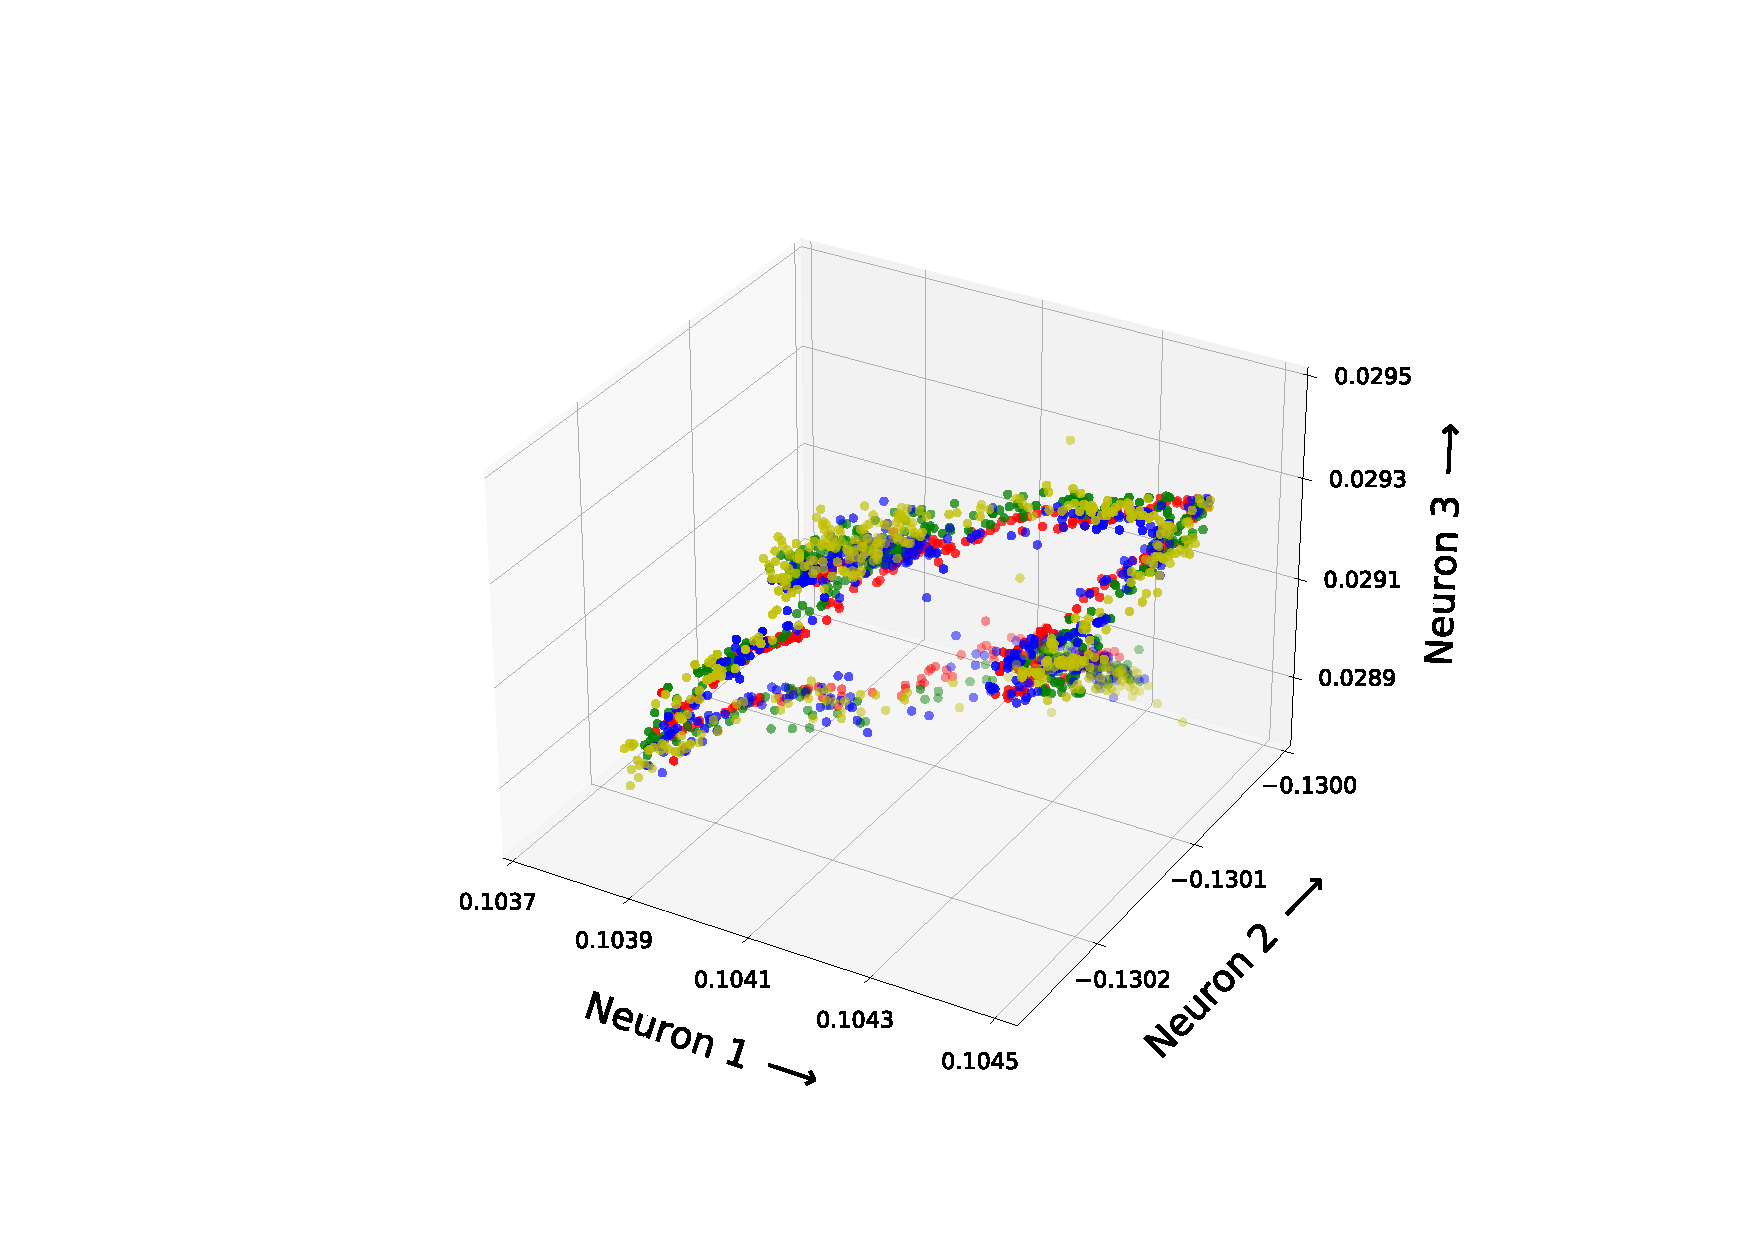
\includegraphics[width=.47\textwidth]{GAMMA_Influence_real_data/P_mech_X_data_distribution_0_GAMMA_0_05.pdf}
  \hspace{.4cm}
  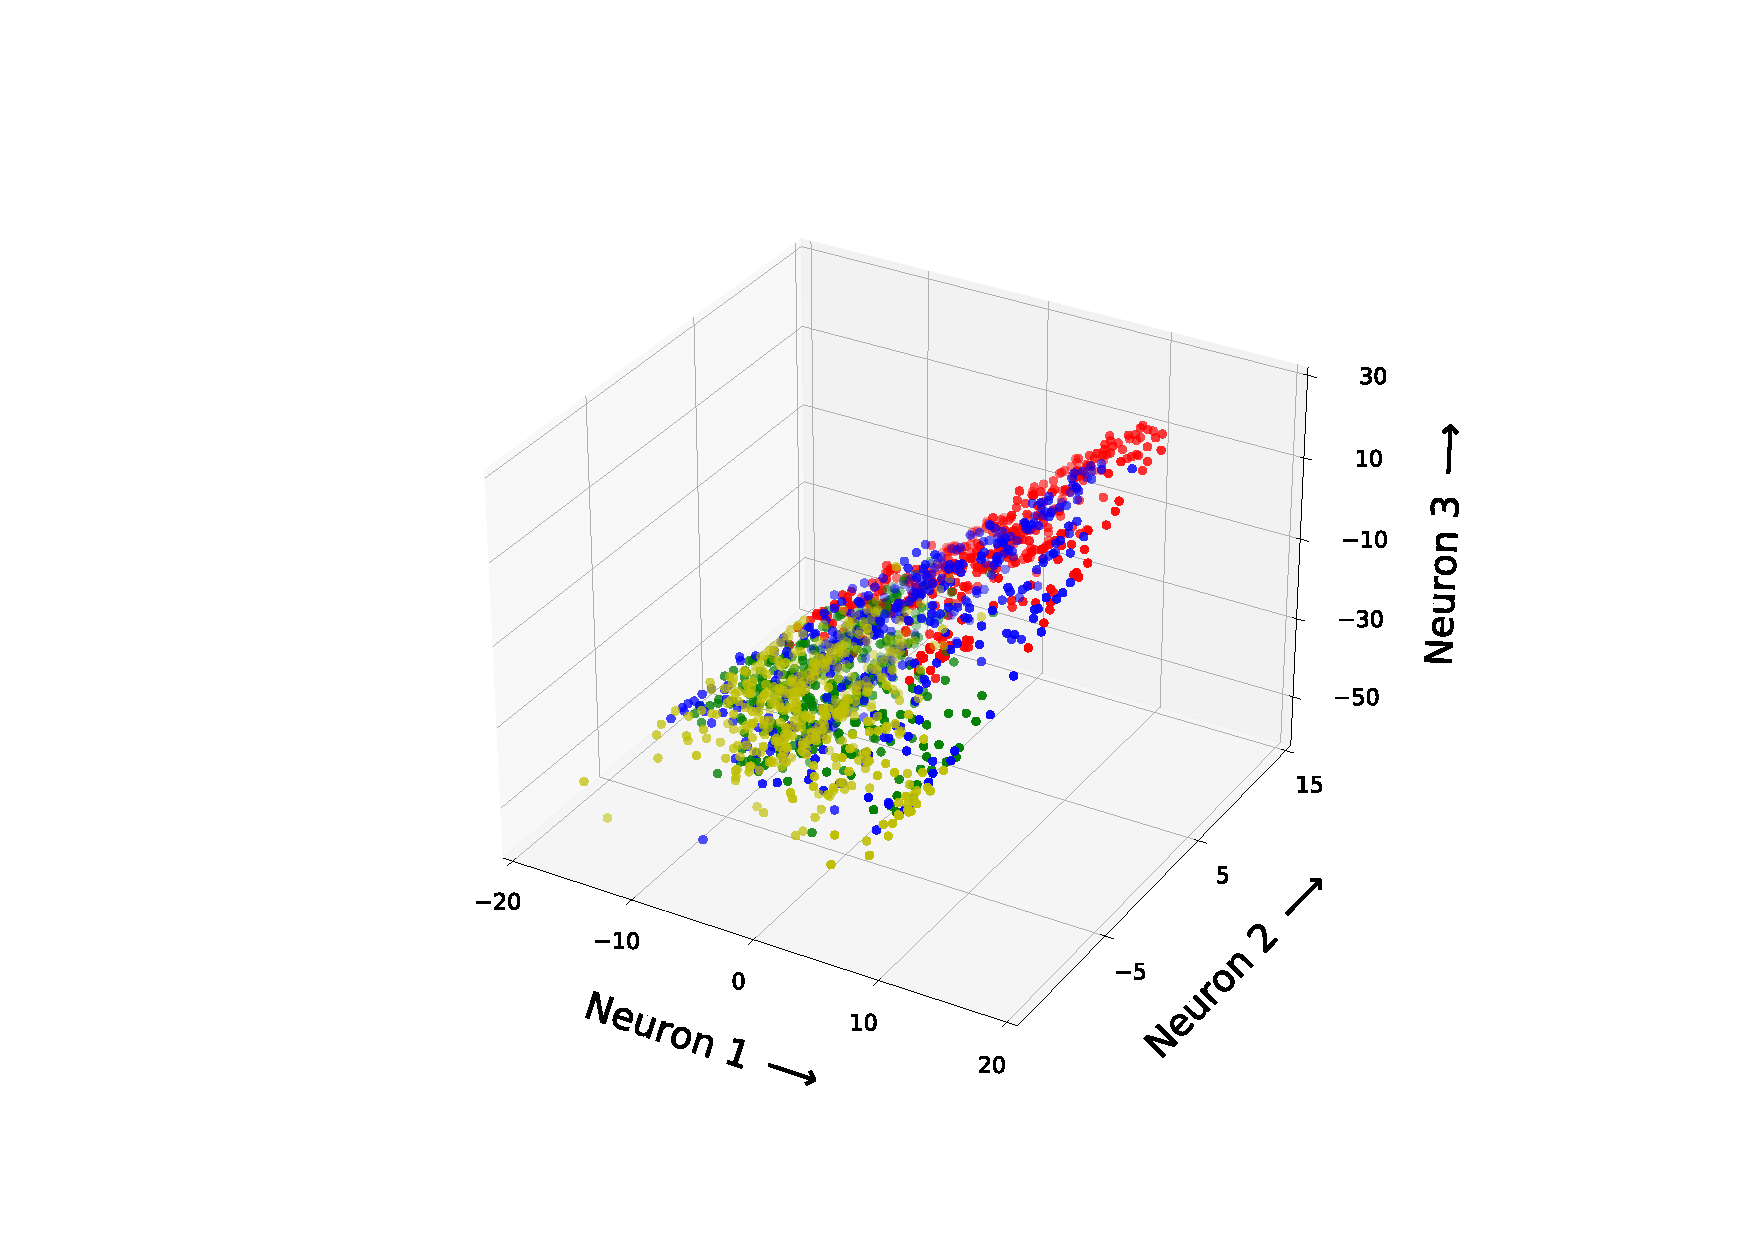
\includegraphics[width=.47\textwidth]{GAMMA_Influence_real_data/P_mech_X_data_distribution_80_GAMMA_0_05.pdf}

  \vspace{.1cm}

  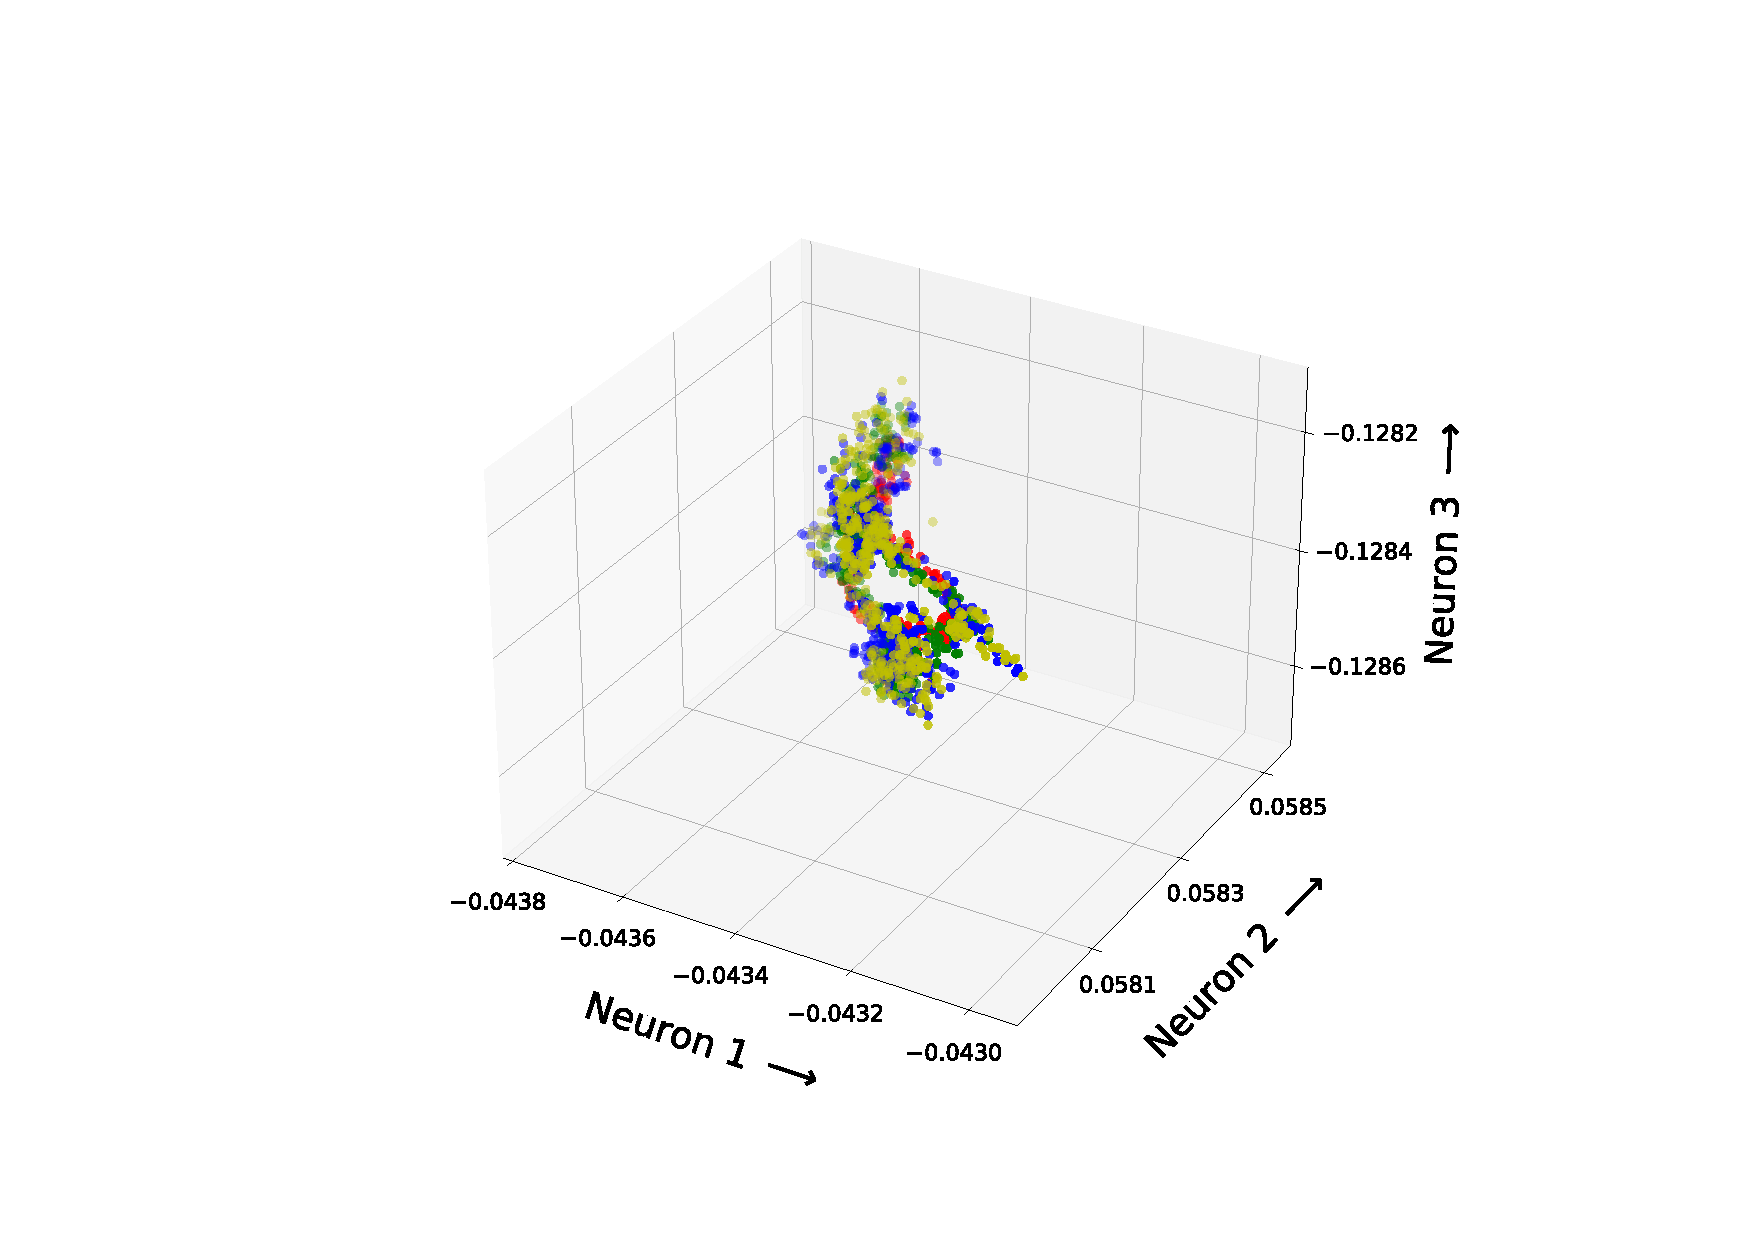
\includegraphics[width=.47\textwidth]{GAMMA_Influence_real_data/P_mech_X_data_distribution_0_GAMMA_1_0.pdf}
  \hspace{.4cm}
  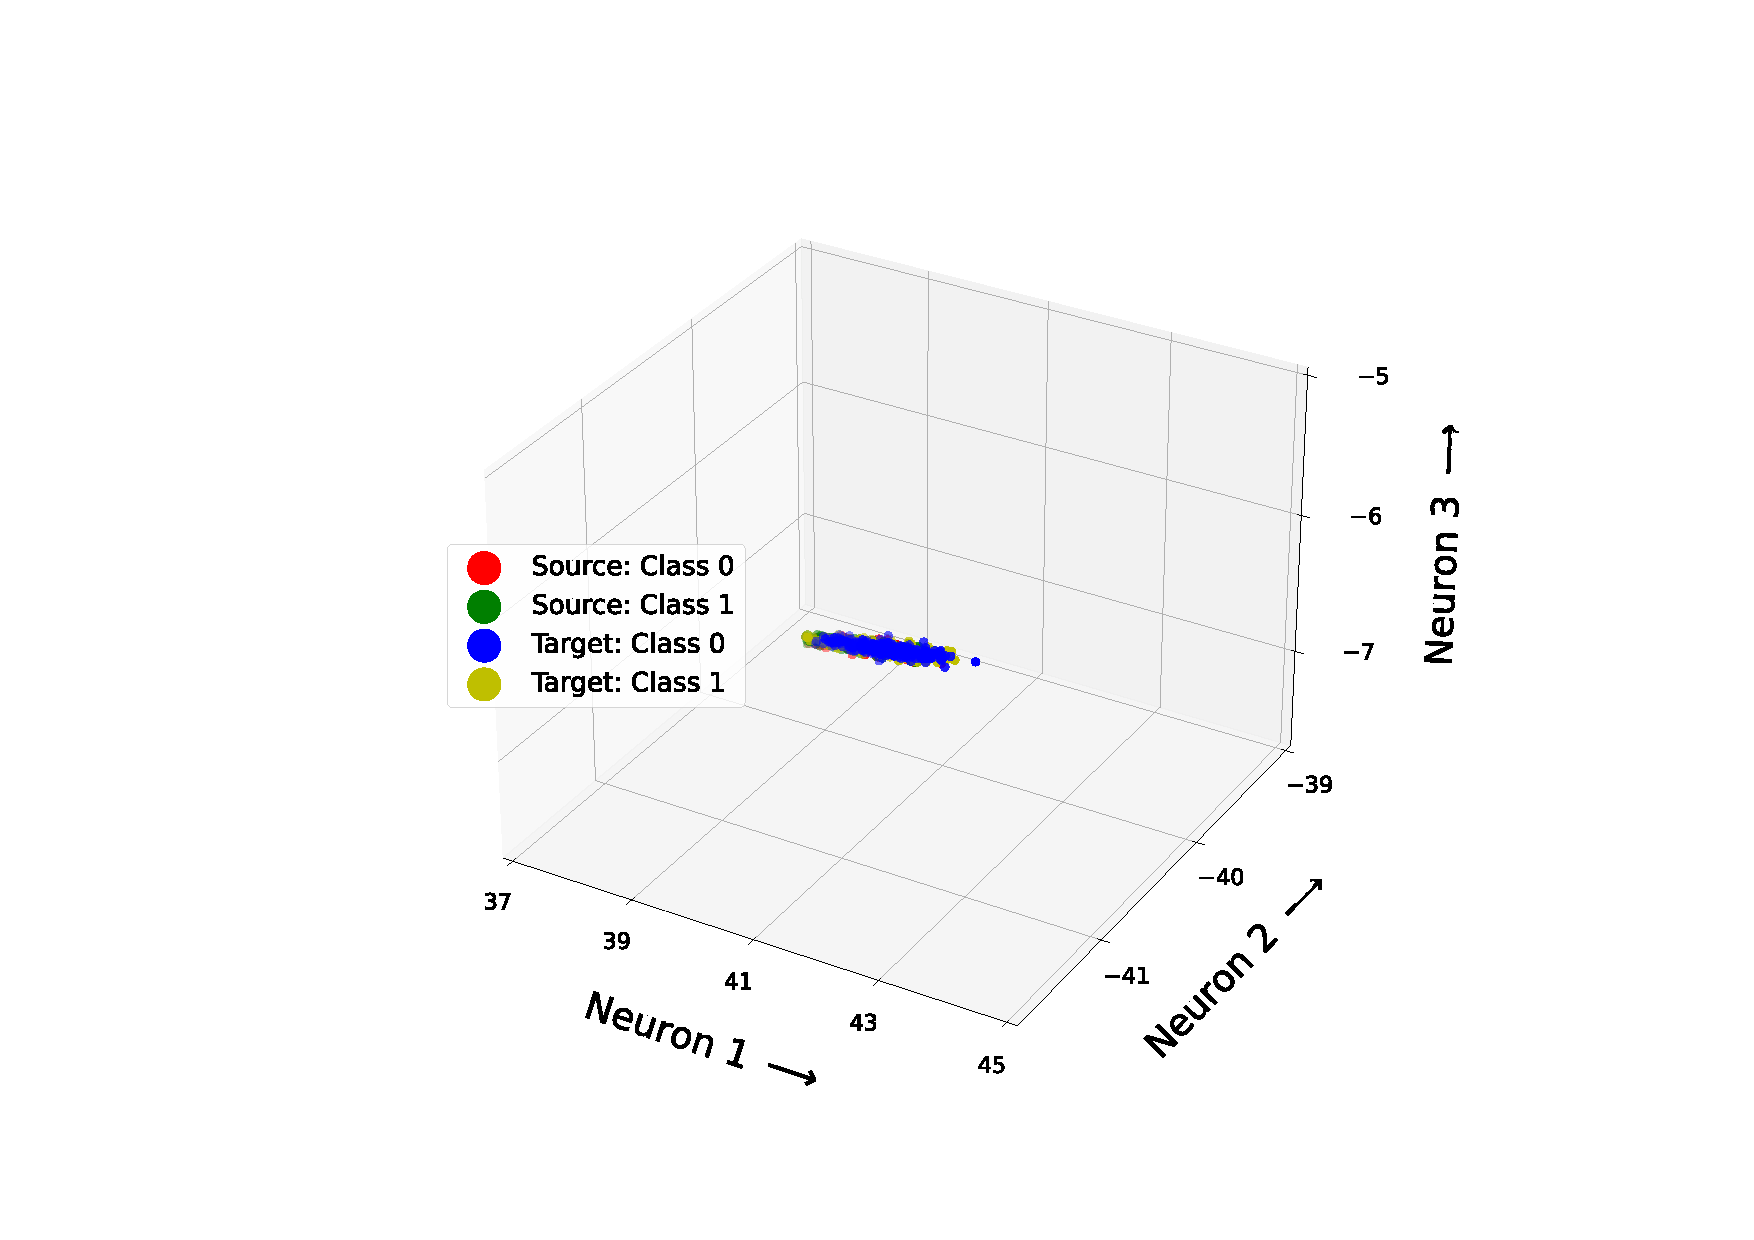
\includegraphics[width=.47\textwidth]{GAMMA_Influence_real_data/P_mech_X_data_distribution_80_GAMMA_1_0.pdf}

  \vspace{.1cm}

  \caption{Data  distribution:  Influence  of  GAMMA  on  Training with D:P\_mech./X:  GAMMA  =  0  (top),GAMMA = 0.05 (middle), GAMMA = 1 (bottom)}
  \label{fig:distribution_GAMMA_influence_real_data}
\end{figure}


\subsection{Influence of Latent Feature Space Choice on the PHM Performance}\label{ch:Influence_Layer_real_dataset}
This section analyses the effects of different MMD latent feature space choices on the model training. Table \ref{tab:MMD_layer_choice} compares the CNN MMD, FC MMD and FULL MMD model. All models were trained on the D:I soll/X signal with a MMD-loss with GAMMA of 1. The experiments were repeated five times. Fig. \ref{fig:target_accuracy_MMD_layer} shows the development of the target accuracy throughout the training. When the MMD-loss is just applied in the FC layers, the training collapses in two of the five experiments (row 3 $\&$ 5). In the other three cases the accuracy has the slight tendency to decrease during the training. Compared to the FULL MMD model the CNN MMD model shows worse reproducibility in the training curves. In some of the CNN MMD experiments the target accuracy is increasing and in some decreasing during the training. Often, the fluctuations on the validation data are not reduced properly throughout the training. The FULL MMD model training seems to be more stable. The fluctuations on the validation data seem to be a little lower and the learning curves. In the course of this evaluation the final model is picked based on the model performance on the target validation dataset. In the real-world the target labels are often unknown. In this case the final model is picked in the end of the training or based on the source domain performance. When the model's performance decreases throughout the training or fluctuates a lot, it is not possible to find the best model like it is done in this thesis. For this reason the importance of a stable model training should not be underestimated. 

\begin{figure}[htp]
  \centering

  \includegraphics[width=.32\textwidth]{MMD_LAYER_influence_real_data/CNN_MMD/Accuracy_Target_Domain_1.pdf}
  \hspace{.1cm}
  \includegraphics[width=.32\textwidth]{MMD_LAYER_influence_real_data/FC_MMD/Accuracy_Target_Domain_1.pdf}
  \hspace{.1cm}
  \includegraphics[width=.32\textwidth]{MMD_LAYER_influence_real_data/FULL_MMD/Accuracy_Target_Domain_1.pdf}

  \vspace{.3cm}

  \includegraphics[width=.32\textwidth]{MMD_LAYER_influence_real_data/CNN_MMD/Accuracy_Target_Domain_2.pdf}
  \hspace{.1cm}
  \includegraphics[width=.32\textwidth]{MMD_LAYER_influence_real_data/FC_MMD/Accuracy_Target_Domain_2.pdf}
  \hspace{.1cm}
  \includegraphics[width=.32\textwidth]{MMD_LAYER_influence_real_data/FULL_MMD/Accuracy_Target_Domain_2.pdf}

  \vspace{.3cm}

  \includegraphics[width=.32\textwidth]{MMD_LAYER_influence_real_data/CNN_MMD/Accuracy_Target_Domain_3.pdf}
  \hspace{.1cm}
  \includegraphics[width=.32\textwidth]{MMD_LAYER_influence_real_data/FC_MMD/Accuracy_Target_Domain_3.pdf}
  \hspace{.1cm}
  \includegraphics[width=.32\textwidth]{MMD_LAYER_influence_real_data/FULL_MMD/Accuracy_Target_Domain_3.pdf}
  
    \vspace{.3cm}

  \includegraphics[width=.32\textwidth]{MMD_LAYER_influence_real_data/CNN_MMD/Accuracy_Target_Domain_4.pdf}
  \hspace{.1cm}
  \includegraphics[width=.32\textwidth]{MMD_LAYER_influence_real_data/FC_MMD/Accuracy_Target_Domain_4.pdf}
  \hspace{.1cm}
  \includegraphics[width=.32\textwidth]{MMD_LAYER_influence_real_data/FULL_MMD/Accuracy_Target_Domain_4.pdf}
  
    \vspace{.3cm}
    
  \includegraphics[width=.32\textwidth]{MMD_LAYER_influence_real_data/CNN_MMD/Accuracy_Target_Domain_5.pdf}
  \hspace{.1cm}
  \includegraphics[width=.32\textwidth]{MMD_LAYER_influence_real_data/FC_MMD/Accuracy_Target_Domain_5.pdf}
  \hspace{.1cm}
  \includegraphics[width=.32\textwidth]{MMD_LAYER_influence_real_data/FULL_MMD/Accuracy_Target_Domain_5.pdf}


  \caption{Target Accuracy: Influence of MMD layer Choice on Training: CNN MMD (left), FC MMD (middle), FULL MMD (right)}
  \label{fig:target_accuracy_MMD_layer}
\end{figure}


\subsection{PHM Performance}\label{ch:PHM_performance}
In this chapter the utility and applicability of the presented models are tested in a real world task. In each epoch, the models are evaluated based on the balanced accuracy on the target domain validation dataset. Throughout the training the best performing model is stored. These models are then tested and compared on an unseen target domain test dataset. In a first step, each model is applied on all of the 49 signals without using any MMD-loss. In a second step, 7 promising signals with high classification accuracies were picked for further testing. These signals were then used to evaluate FULL MMD, FC MMD and CNN MMD. Each model was optimized with different GAMMAs (0.05 $\&$ 0.5 $\&$ 1). The FULL MMD, FC MMD and CNN MMD were used with three different GAMMAs (0.05 $\&$ 0.5 $\&$ 1). Each of these 9 models and the baseline model were tested 5 times on the 7 signals. Table \ref{tab:Mean_Accuracy} shows the target accuracy, averaged over all 5 equally executed experiments. For 4 of the 7 signals the FULL MMD and for the other 3 the CNN MMD model performed best. The FC MMD models never outperformed the other MMD-based models. Compared to the baseline model the MMD-based models were able to increase the accuracy with up to 10.18$\%$. Table \ref{tab:Variance_Accuracy} shows the target accuracy variances for all models and selected signals. The best performing model usually shows low to average variances. A low variance verifies a high degree of reproducibility in the repeated experiments. This demonstrates the meaningfulness of the results and proves the applicability and utility of MMD-losses for reducing the domain discrepancy in PHM related tasks. Table \ref{tab:Average_Variance_Accuracy} shows the average variance over all 105 experiments with MMD-based models and 35 experiments with baseline models. From the MMD-based models, the FULL MMD has the lowest and the FC MMD the highest average target accuracy variance. This shows that the FULL MMD model has the highest reproducibility. As mentioned in the results of the dummy dataset, a reason might be the contradicting training goals when evaluating the MMD as well as the source CE-loss just in the FC layers. This might lead to instabilities and a training which is more prone to getting stuck in local minima. The signals recorded during the constant and direction change excitement of the machines are especially suitable for the PHM of BSDs. 

\begin{comment}
Windowing functions split the recorded data in shorter sequences. The generated windows should capture the degradation related patterns of the vibration signals. For this reason, the windows should be adapted according to the consistency and periodicity of the data. In this thesis a window size of 1024 was chosen. The windowing requirements are different for the different machine excitements (constant speed excitement, direction change excitement and sweep excitement). The windows are too short to capture one whole period of of forward and backward motion in the data recorded during constant speed machine excitement. The data can be separated in phases of constant speed and direction change, which each contains roughly 1000 datapoints. The windows are of equal size as the described phases in the data. Since the windows are not synchronized with those phases, they overlap to a large extent but do not cover them perfectly. The windows are big enough to capture several periods of forward and backward movements in data recorded during direction change excitement. When exciting the machine with a sweep signal the PHM system should better process the whole corresponding vibration signal. It is important to capture the changing frequencies and amplitudes during the complete sweep excitement. The best PHM results were achieved on data recorded during constant speed and  direction change excitement of the machine. This shows that the windowing did not work very well on the data recorded during sweep excitement. Generally, when choosing the window size, there is a trade-off between the window size and the number of windows generated from the data. Both extremes (few big windows and numerous small windows) might lead to problems during the training. The PHM results can probably be improved by an intelligent and adaptive preprocessing to generate suitable and synchronized data windows. Azamfat et al \cite{AZAMFAR2020103932} present such an approach. They apply a constant excitement to the machine and separate the data BSD phases of constant velocity direction change movement. The PHM system just relies on the data recorded during BSD constant velocity. The signals D:I\_ist/X (actual electrical power), D:I\_soll/X (target electrical power) and D:P\_mech./X (mechanical power) coming from the controller show high potential for the PHM task. The most suitable accelerometer installation is the one on the BSD nut. Pandahare et al \cite{Pandhare2021} discovered similar results. Often in real operational scenarios such an installation is impractical \cite{Pandhare2021}. Alternatively to the BSD nut position, this thesis shows, that the top LGS achieves better PHM results than the bottom one.
\end{comment}


\begin{sidewaystable}
\begin {table}[H]
\centering
\begin{tabular}{llllllllll}
  \toprule
  Model          & GAMMA    & D:I\_ist/X & D:I\_soll/X & D:P\_mech./X & C:z\_top & C:z\_nut & D:x\_nut & D:z\_top \\
  \midrule
  
  \vspace{1cm}
  
    \thead{BASE- \\ LINE}  & -      & 70.08 & 75.62 & 74.7 & 69.14 & 57.4 & 58.74 & 57.88\\


 
                            & 0.05   & 71.56 & 75.42 & \textbf{78.96} & 72.36 & 58.10 & 49.52 & \textbf{62,64}\\
    \thead{FULL \\ MMD}     & 0.5    & 73.78 & 74.84 & 52.78 & \textbf{75.92} & \textbf{64.76} & 50.52 & 49,94\\
    
    \vspace{1cm}
    
                            & 1      & 72.98 & 75.18 & 49.80 & 74.12 & 57.02 & 50.62 & 50.52\\


                            & 0.05   & 73.60 & 76.38 & 74.98 & 71.36 & 57.48 & 52.44 & 61.3\\
    \thead{FC \\ MMD}       & 0.5    & 70.74 & 74.86 & 72.62 & 69.32 & 59.76 & 50.12 & 53.22\\
    
    \vspace{1cm}
    
                            & 1      & 73.42 & 65.46 & 76.96 & 62.34 & 58.86 & 50.92 & 53.96\\

                            & 0.05   & 71.62 & \textbf{76.44} & 51.80 & 73.20 & 59.30 & 58.04 & 53.82\\
    \thead{CNN \\ MMD}      & 0.5    & \textbf{73.90} & 75.86 & 51.58 & 72.28 & 55.76 & 68.04 & 51.72\\
                            & 1      & 73.80 & 73.82 & 51.12 & 72.18 & 54.28 & \textbf{68.92} & 51.28\\
 \addlinespace
 \hline
 \thead{MMD\\GAIN:} &  & +3.82 & +0.82 & +4.26 & +6.78 & +7.36 & +10.18 & +4.76\\
 
  \bottomrule
\end{tabular}
\caption {Mean target test accuracy (\%)} \label{tab:Mean_Accuracy} 
\end {table}
\end{sidewaystable}

\begin{sidewaystable}
\begin {table}[H]
\centering
\begin{tabular}{llllllllll}
  \toprule
  Model          & GAMMA    & D:I\_ist/X & D:I\_soll/X & D:P\_mech./X & C:z\_top & C:z\_nut & D:x\_nut & D:z\_top  \\
  \midrule

    \vspace{1cm}

    \thead{BASE- \\ LINE}   & -      & 2.07 & 0.27 & 2.20 & 2.55 & 1.11 & 1.04 & 1.22\\
 
                            & 0.05   & 1.06 & 0.74 & \textbf{1.79} & 1.80 & 2.04 & 1.39 & \textbf{2.48}\\
    \thead{FULL \\ MMD}     & 0.5    & 0.72 & 1.44 & 3.33 & \textbf{1.72} & \textbf{1.42} & 1.23 & 1.02\\
    
    \vspace{1cm}  
    
                            & 1      & 0.76 & 0.81 & 0.87 & 6.06 & 5.57 & 0.96 & 0.79\\



                            & 0.05   & 1.96 & 0.61 & 1.86 & 1.82 & 1.63 & 3.86 & 1.60\\
    \thead{FC \\ MMD}       & 0.5    & 1.34 & 0.72 & 11.06 & 6.42 & 2.28 & 0.45 & 3.14\\
    
    \vspace{1cm}
    
                            & 1      & 0.96 & 12.01 & 5.46 & 8.18 & 2.13 & 0.93 & 2.70\\
                            & 0.05   & 2.13 & \textbf{0.53} & 2.39 & 1.12 & 4.01 & 4.18 & 7.26\\
    \thead{CNN \\ MMD}      & 0.5    & \textbf{0.25} & 1.57 & 1.08 & 1.22 & 3.27 & 3.51 & 3.22\\
                            & 1      & 0.51 & 1.25 & 2.02 & 2.51 & 4.54 & \textbf{2.54} & 2.34\\
  \bottomrule
\end{tabular}
\caption {Standard deviation target test accuracy (\%)} \label{tab:Variance_Accuracy} 
\end {table}
\end{sidewaystable}


\begin {table}[H]
\centering
\begin{tabular}{lllll}
  \toprule
  Model & BASE-LINE & FULL MMD & FC MMD & CNN MMD\\
  \midrule
  AVG VARIANCE & 1.50 & 1.81 & 3.39 & 2.45\\
  \bottomrule
\end{tabular}
\caption {Average standard deviation target test accuracy (\%)} \label{tab:Average_Variance_Accuracy} 
\end {table}

